%%%%%%%%%%%%%%%%%%%%%%%%%
%%%%%%%%%%%%%%%%%%%%%%%%%
% !TeX encoding = UTF-8
% !TeX program = xelatex
% !Mode:: "TeX:UTF-8"

\documentclass[twoside]{thesis-cls-Miya}

\usepackage{float}
\usepackage{placeins}
\usepackage{fancyvrb}
\usepackage{pdfpages}

\usetikzlibrary{shapes,shapes.geometric,arrows.meta}

\raggedbottom
\hbadness=10000
\newcommand{\thesisfigureplaceholder}[2][0.90\textwidth]{%
  \begingroup
  \setlength{\fboxsep}{12pt}%
  \fbox{%
    \parbox[c][4.8cm][c]{\dimexpr#1-2\fboxsep-2\fboxrule\relax}{%
      \centering
      \textbf{图片占位符}\\[0.6em]
      #2\\[0.6em]
      \small 后续按项目实际重新绘制
    }%
  }%
  \endgroup
}
\newcommand{\thesisfigportrait}[1]{%
  \includegraphics[width=0.84\textwidth,height=0.72\textheight,keepaspectratio]{#1}%
}
\newcommand{\thesisfigflow}[1]{%
  \includegraphics[width=0.86\textwidth,height=0.56\textheight,keepaspectratio]{#1}%
}
\newcommand{\thesisfigwide}[1]{%
  \includegraphics[width=0.94\textwidth,height=0.42\textheight,keepaspectratio]{#1}%
}
\newcommand{\thesisfigscreen}[1]{%
  \includegraphics[width=0.92\textwidth,height=0.46\textheight,keepaspectratio]{#1}%
}
\newcommand{\thesisfigsmallscreen}[1]{%
  \includegraphics[width=0.78\textwidth,height=0.38\textheight,keepaspectratio]{#1}%
}

\renewcommand{\topfraction}{0.95}
\renewcommand{\bottomfraction}{0.95}
\renewcommand{\textfraction}{0.05}
\renewcommand{\floatpagefraction}{0.95}
\setlength{\textfloatsep}{10pt plus 2pt minus 4pt}
\setlength{\floatsep}{8pt plus 2pt minus 2pt}
\setlength{\intextsep}{10pt plus 2pt minus 2pt}
\makeatletter
\setlength{\@fptop}{0pt}
\setlength{\@fpsep}{10pt plus 1fil}
\setlength{\@fpbot}{0pt plus 1fil}
\pretocmd{\section}{\FloatBarrier}{}{}
\pretocmd{\subsection}{\FloatBarrier}{}{}
\pretocmd{\subsubsection}{\FloatBarrier}{}{}
\makeatother
\newcommand{\appendixspecialcenter}[1]{%
  \clearpage
  \phantomsection
  \addcontentsline{toc}{chapter}{#1}
  \markboth{#1}{}
  \vspace*{-5ex}%
  \begin{center}
    {\zihao{1}\bfseries\songti #1}
  \end{center}
  \vskip 0em%
}
\newcommand{\appendixspecialcenternotoc}[1]{%
  \clearpage
  \phantomsection
  \markboth{#1}{}
  \vspace*{-5ex}%
  \begin{center}
    {\zihao{1}\bfseries\songti #1}
  \end{center}
  \vskip 0em%
}
\begin{document}

\title{基于技术交流群体的智能聊天室}
\titleB{设计与实现}
\englishtitleA{Design and Implementation of an}
\englishtitleB{Intelligent Chat Room for Technical}
\englishtitleC{Communication Groups}

\author{麦旻轩}

\kongF{2214100540}
\kongG{22软件工程1班}
\kongH{刘利 副教授}
\kongI{2026年4月19日}

\maketitle

\frontmatter

\begin{abstract}
面向技术讨论的在线交流，不只是发送普通文本消息，还经常伴随代码片段、报错日志、接口参数、文件附件和阶段性结论。通用聊天工具虽然能够完成基础沟通，但在历史回读、技术内容展示和讨论结果沉淀方面仍然不够贴合开发场景。针对这些问题，设计并实现了一套面向技术交流群体的智能聊天室系统 Mini-Chat-Bar。

系统采用前后端分离架构。前端使用 Vue 3 构建 Web 界面，并通过 Electron 封装桌面端；后端基于 Node.js、Express 和 Socket.IO 实现接口服务与实时通信；MongoDB 用于保存用户、房间、私聊消息、聊天室消息、收藏和 AI 相关数据。围绕技术交流场景，系统实现了注册登录、私聊、聊天室、文件分享、历史回读、收藏管理、AI 问答和讨论总结等功能。AI 模块采用检索增强生成思路，在聊天室问答时结合历史消息索引结果组织上下文，使返回内容尽量贴近当前讨论。
在部署方式上，系统也保留了本地私有化部署思路，业务服务与数据库可按 Docker 容器方式部署在个人开发机或团队内网环境中，便于控制消息数据和业务配置的留存位置。

测试结果表明，系统已经跑通主要业务链路。登录、资料读取、消息列表和收藏列表等普通接口保持毫秒级响应；在单机本地环境下，100 个 Socket 客户端广播成功率保持 100\%；AI 问答和讨论总结能够正常返回并写入历史记录，但耗时明显高于本地业务接口，主要受外部模型服务影响。整体来看，完成的系统已经能够满足课程项目和毕业设计演示需求。

\keywords{智能聊天室；实时通信；AI助手；Vue 3框架；RAG技术}
\end{abstract}

\begin{englishabstract}
Technical-oriented online communication involves not only plain text messages but also code snippets, error logs, API parameters, file attachments, and interim conclusions. General-purpose chat tools can support basic communication, but they are less suitable for developer scenarios that require efficient history review, technical content display, and knowledge retention. To address this gap, this paper designs and implements Mini-Chat-Bar, an intelligent chat system for technical communities.

The system adopts a separated front-end and back-end architecture. The front end uses Vue 3 for web interfaces and Electron for desktop packaging, while the back end uses Node.js, Express, and Socket.IO for API services and real-time communication. MongoDB stores users, chat rooms, private messages, group messages, favorites, and AI-related data. For technical communication scenarios, the system supports user authentication, private messaging, group chat, file sharing, message history review, favorite management, AI-based question answering, and discussion summarization. The AI module uses retrieval-augmented generation to incorporate indexed historical messages into the current context. The system also supports local private deployment through Docker containers on personal development machines or internal networks, which helps control data storage and configuration.

Experimental results show that the system completes the main business workflows. Common interfaces such as login, profile retrieval, message lists, and favorites maintain millisecond-level response times. In single-machine tests, message broadcasting remained stable with 100 Socket clients. AI-based question answering and discussion summarization worked correctly and were recorded in message history, but their latency was significantly higher than local services because they depended on external model services. Overall, the system meets the needs of course projects and graduation project demonstrations.

\englishkeywords{Intelligent Chat Room; Real-time Communication; AI Assistant; Vue 3; RAG Technology}
\end{englishabstract}

\tableofcontents

\mainmatter

% 引入各章节
\chapter{绪论}

\section{研究背景与意义}

面向技术讨论的在线交流，与日常社交聊天并不一样。在课程项目联调、接口排错、版本确认和开源协作等场景中，参与者反复交换的往往是代码片段、报错日志、接口参数、测试结果和临时结论。消息一多，真正有用的内容就容易被后续讨论淹没，后来加入的人也难以及时接上上下文，只能重新追问，沟通成本随之增加。

现有聊天工具能够承担部分交流任务，但在技术讨论场景中仍有明显不足。通用社交软件偏向日常沟通，对技术内容展示、历史回看和结果留存考虑不多；功能更完整的协作平台覆盖面虽广，却往往带来更高的部署和使用成本。因而，围绕讨论过程组织消息、保留关键结论并支持后续回看，已成为技术交流系统的现实需求\cite{textchat2024}。如果系统还能支持个人电脑或团队内网中的本地部署，就能更好控制消息数据和讨论记录的留存位置。技术讨论中还常有一类高频需求：遇到陌生术语、报错信息或代码片段时，希望直接在当前界面完成划词解释，而不是反复切出聊天窗口搜索。

与此同时，大语言模型和检索增强技术的发展，也让聊天系统有了新的扩展方向。AI 的价值不在于脱离上下文单独回答问题，而在于结合当前会话历史继续参与问答，在需要时完成问题梳理、阶段总结和术语解释\cite{qaoverview2025}。这样一来，用户不必在聊天工具、搜索工具和独立 AI 工具之间来回切换，沟通链路更短，信息也更容易沉淀。因此，设计一套面向技术交流群体的智能聊天室系统，具有较强的实际应用价值和明确的研究意义。

\section{国内外研究现状}

\subsection{即时通讯系统与协作平台的发展}

现有即时通信系统的研究，早已不只停留在“发送一条消息”这一层面。消息留痕、群组组织、文件共享、权限控制和安全通信，已经逐渐成为这类系统的常见能力。针对具体使用场景对聊天系统做定制化裁剪，也是近年来较常见的实现思路。

这对本文的启发比较直接。技术交流群体需要的不是一套笼统的大平台，而是围绕问题讨论本身展开的轻量化工具：消息要清楚，历史要能回看，关键内容要能保留下来，后加入的人也要能尽快看懂前文。

\subsection{Web实时通信技术研究现状}

在 Web 场景下，实时通信问题已经有比较成熟的处理方式。早期轮询和长轮询能够实现近实时效果，但请求频率较高，服务端压力也更明显。WebSocket 普及之后，浏览器与服务器可以保持持续连接，消息推送、在线状态同步和多人广播都更适合放在这一机制下完成\cite{pollingssews2026}。

从工程角度看，当前更常见的做法是把普通请求和实时连接分开使用：前者负责登录鉴权、数据读取和消息落库，后者负责在线状态、增量通知和广播同步。这样处理的好处很务实，链路更清楚，排查问题也更直接。本文的系统设计也是建立在这一思路之上。

\subsection{AI辅助交流技术研究现状}

近年的 AI 研究已经从单纯追问“模型能不能回答问题”，逐渐转向“模型怎样结合外部信息更稳定地回答问题”。已有研究表明，大语言模型在问答、归纳和文本生成方面表现出较强能力，但当输入缺少上下文时，回答仍然容易变得空泛，甚至偏离原问题\cite{gpt4report2023}。

为了解决这一问题，检索增强生成成为近几年较受关注的方向。它的基本思路不是让模型只依赖参数记忆，而是在生成之前补充与当前问题相关的外部信息，从而提高回答的相关性和可用性\cite{ragsurveycn2025}。

针对开发者聊天场景中的阶段总结与多轮追问，已有研究也开始关注摘要方法、对话历史管理以及长上下文利用问题\cite{devchatsummary2025}。

对技术交流场景来说，这一点尤其重要。同一句提问，放在不同聊天室、不同项目阶段里，含义可能完全不同。AI 如果不能接入历史讨论，就很难真正理解当前问题。也正因为如此，本文把 AI 看成聊天链路的一部分，而不是一个脱离场景的独立问答入口。

\section{研究内容与目标}

本文以本人设计并实现的 Mini-Chat-Bar 为对象，围绕技术交流群体的使用特点，完成一套轻量化智能聊天室系统的分析、设计、实现与测试。研究内容主要包括四个方面：一是结合课程项目协作、联调排错和日常技术讨论等场景，梳理目标用户、业务流程与核心需求；二是完成系统总体架构、功能模块和数据组织设计，形成支撑实时通信与 AI 辅助的技术方案；三是实现私聊、聊天室、历史回读、收藏、侧边栏 AI 对话、结合聊天记录的上下文问答、讨论总结与划词解释等功能；四是通过功能测试和性能测试验证系统的可用性与稳定性。

本文的目标不是泛泛讨论“智能聊天”这一概念，而是做出一套能够实际运行的产品原型 Mini-Chat-Bar，并验证它是否适合技术交流场景。该产品既要满足消息收发、历史回看和多人协作等基础交流需要，也要让 AI 以更自然的方式融入讨论过程，例如在侧边栏继续追问、在聊天室里结合历史消息回答问题、对选中的文本做解释，并把有价值的结果保留下来，减少重复沟通。

从价值上看，这套系统可以为课程项目、小型开发团队和技术兴趣社群提供一套门槛相对较低的交流工具，帮助用户更快定位问题、理解术语并回看已有结论。从实现特点上看，本文的侧重点不在于提出新的模型算法，而在于把即时通信、历史消息组织和 AI 辅助放到同一产品链路里：AI 不是独立悬浮在外的问答窗口，而是能够利用聊天记录参与当前讨论，回答结果又能继续被引用、收藏和回看。这种围绕具体使用场景进行整合的做法，也是本课题相对有新意、同时更有现实意义的地方。

\section{论文结构安排}

后文按“需求分析、总体设计、具体实现、测试验证”的顺序展开。

第一章为绪论，交代课题背景，并梳理即时通信、实时通信与 AI 辅助相关的研究现状。

第二章介绍相关技术，说明前端界面组织、后端服务处理、实时通信、数据存储及 AI 检索增强等技术在本项目中的使用方式。

第三章进行系统需求分析，围绕目标用户、典型场景、功能需求与非功能需求，明确系统需要完成和暂不实现的内容。

第四章阐述系统总体设计，包括整体架构、模块划分、数据库设计，以及认证、消息流转、聊天室交互和 AI 辅助等核心流程。

第五章说明系统实现，结合前后端代码与界面，介绍用户、聊天、聊天室、收藏、AI 模块及 Electron 桌面端功能的具体实现。

第六章给出系统测试，从测试环境、功能测试和性能测试三个方面验证运行情况，展示接口、实时通信和 AI 调用链路的测试结果。

第七章为总结与展望，归纳已完成的工作，并说明后续仍可继续改进的方向。

论文正文后的附录统一收录任务书、开题/中期检查、指导记录、审批表与成绩评定等过程性材料，相关内容可结合\hyperref[app:materials]{附录}查阅。

\chapter{开发技术简介}

\section{技术选型与架构概述}

本章不再把项目中用到的技术逐个写成教材式介绍，而是围绕 Mini-Chat-Bar 的实际需求说明技术选型的理由。开发过程中，系统最先暴露出的并不是某个单独页面的问题，而是几类能力需要同时成立：既要完成登录、资料读取、消息保存和收藏回看等稳定的数据处理，也要支撑私聊提醒、聊天室广播、在线状态变化和 AI 增量回复这类实时交互，还要兼顾桌面端通知与托盘常驻等本地能力。单靠一种技术很难把这些事情都处理好，因此项目最终采用了前后端分层、实时通信与数据存储协同配合的方案。

如图~\ref{fig:2-1}所示，系统整体可以分为接入层、前端应用层、服务层以及数据与智能辅助层。

\begin{figure}[H]
\centering
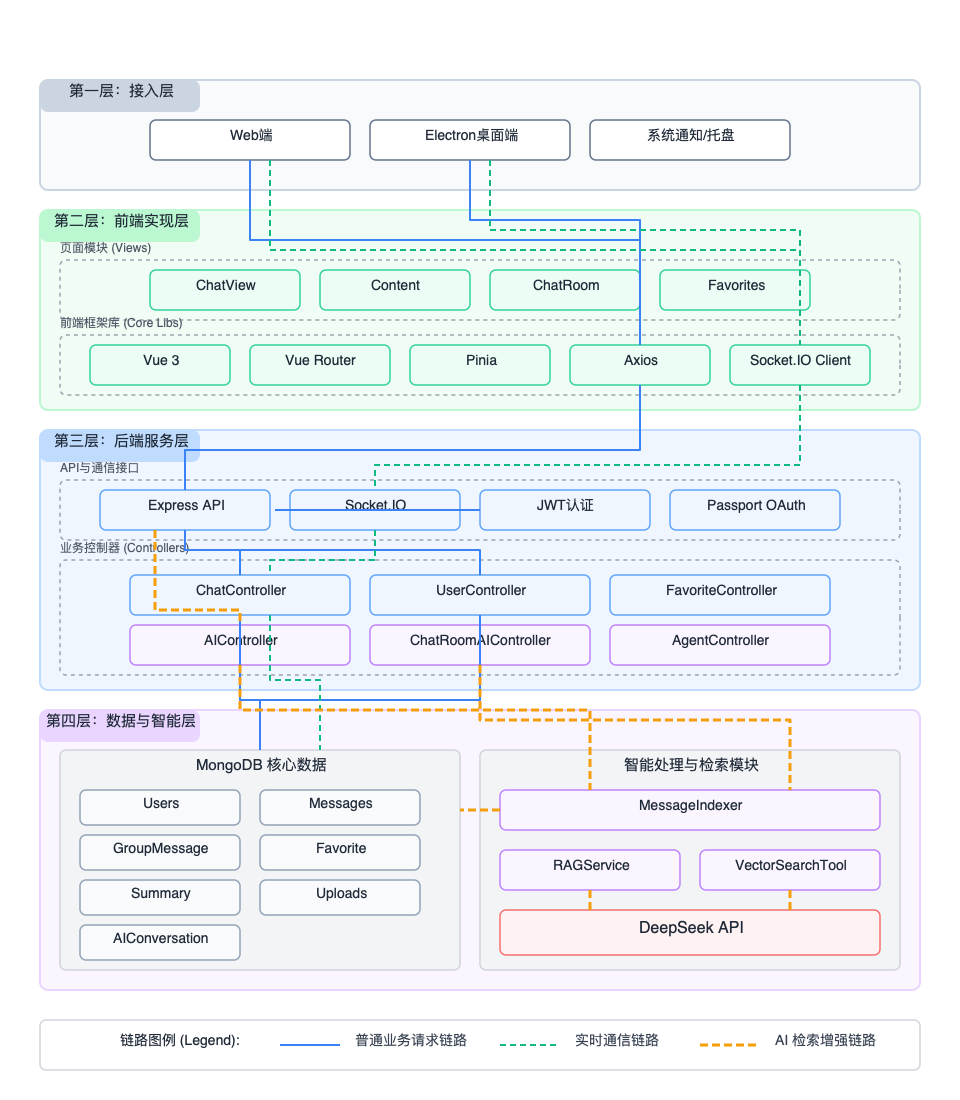
\includegraphics[width=0.76\textwidth,height=0.60\textheight,keepaspectratio]{img/图2_1.png}
\caption{系统技术架构图}
\label{fig:2-1}
\end{figure}

这样的划分不是为了把架构图画得复杂，而是因为系统中的不同任务确实需要不同链路来承担。前端主要负责界面呈现、会话切换和用户交互；服务层负责权限校验、业务处理和消息流转；数据层负责用户资料、聊天记录和收藏内容的持久化；AI 服务层则负责问答、总结和解释等增强能力。这样拆开以后，稳定的数据读写与需要即时反馈的实时交互各走合适的路径，系统结构会更清楚，后续实现和排查问题也更直接。

图~\ref{fig:2-1}并不是套用通用模板得到的，而是依据本系统已经完成的功能结构整理出来的。图中把用户管理、即时通信、聊天记录、文件管理和 AI 辅助几个部分放在同一套架构下，说明它们如何共同支撑私聊、聊天室、收藏回看和智能问答等功能。这样的表达方式也为后续章节展开总体设计、功能实现与测试验证提供了统一的基础。

\section{前端实现技术}

前端部分最明显的特点，是同一套界面中同时存在登录鉴权、会话切换、实时消息显示、聊天室详情、收藏回看和 AI 辅助等多种交互。Vue 3 在这个项目里的价值，主要体现在把这些界面拆成职责相对清楚的部分，而不是单纯为了追求新框架\cite{vueguide2026}。聊天主界面采用会话列表、消息区和详情区的三栏结构后，私聊、聊天室和收藏等功能就可以围绕各自的区域展开，界面关系也更容易理清。

状态管理由 Pinia 承担，但并没有把所有界面状态都收进全局。跨页面共享的会话状态和消息数据由状态管理统一维护，局部弹窗、搜索词和短时交互则继续放在组件内部处理。这样的划分更贴合本项目的实际需要，也减少了页面联动时的复杂度\cite{piniadocs2026}。配合 Vue Router 管理页面切换、Vite 支撑开发阶段的快速调试，再结合 Electron 补足托盘、通知和桌面常驻能力，前端部分既能保持 Web 端开发效率，也能满足桌面端展示需求。

Electron 的接入同样是围绕现有页面补能力，而不是另写一套桌面客户端。这样做保留了 Web 界面的复用效率，同时也补上了桌面常驻、消息提醒和窗口切换这些在实际使用和答辩演示中都比较直观的交互能力。

\section{后端服务与实时通信技术}

后端采用 Node.js 和 Express，并不是因为它们在 Web 项目里足够常见，而是因为这个系统从一开始就同时存在两类请求形态：一类是登录、资料读取、消息查询和收藏处理这类可以较快结束的普通请求，另一类是消息发送、在线同步和 AI 流式回复这类会持续交互的链路。把这两类请求放在同一套 JavaScript 运行环境里处理，有利于减少前后端联调时的切换成本\cite{expressdocs2026}。

本项目里 HTTP 和 Socket.IO 的分工很清楚，二者并不是互相替代。普通请求主要负责身份认证、数据读写和结果持久化，实时通道主要负责把新消息、在线状态和增量内容及时同步给在线成员。这样处理的好处很实际：稳定数据通过普通接口处理，实时变化通过长连接同步，既便于保证消息可靠落库，也便于后续定位问题\cite{socketiodocs2026}。

身份认证方面，系统采用 JWT 维护登录状态。无论用户采用邮箱密码、验证码还是第三方登录，后续访问都统一进入同一套鉴权流程。这样处理既方便权限控制，也减少了不同登录方式带来的后端分支复杂度\cite{oauthbcp2025}。

\section{数据存储与消息组织技术}

从数据组织看，虽然私聊消息、聊天室消息、收藏快照、AI 回复和讨论总结最终都会显示在聊天界面里，但它们的结构、读取方式和保存重点并不相同。私聊更强调双方关系下的历史回读，聊天室更强调按房间分页加载和多人共享，收藏更强调快照留存，AI 对话和总结则需要保留上下文信息。基于这种差异，系统采用 MongoDB 存放主要业务数据\cite{mongodbdocs2026}。

结合实际访问路径，系统把用户、聊天室、消息、收藏和 AI 相关数据分别组织，历史消息重点围绕会话或房间读取，收藏内容则便于后续筛选和回看。文件资源与消息记录分开保存，只在消息中保留必要的展示与定位信息。这样的设计不追求形式上的复杂，而是服务于当前项目里最常见的读取与回看需求。

索引设置同样跟着读取方式走。常用查询集中在最近会话、按时间回读历史消息、按房间查看讨论和按用户查看收藏等场景，因此数据库优化也围绕这些高频路径展开。对本科毕业设计的系统规模来说，这样的组织方式已经足够支撑消息分页、历史检索和收藏沉淀等主要功能。

\section{AI辅助技术}

本系统中的 AI 不是附加在聊天界面旁边的演示功能，而是直接参与技术讨论过程。侧边栏 AI 助手更适合单人连续追问，也可以用于对选中的术语、报错信息或代码片段做解释；聊天室内的 AI 问答和阶段总结则面向多人协作，回答结果能够继续留在房间里被所有成员查看和引用。

如果只把用户最后输入的一句话直接交给模型，回答很容易脱离前文。为了解决这个问题，项目在聊天室问答链路中加入了消息索引与检索增强。问答发起前，系统会先从当前房间的历史消息中召回相关讨论，再把这些上下文与用户问题一并提交给模型。这样得到的回答更贴近房间里已经形成的讨论脉络，而不是把每次提问都当作一条孤立的新问题。

考虑到 AI 回复明显慢于普通接口，系统采用流式输出方式逐步返回内容，让提问者和房间成员都能及时看到回答进展。这种做法虽然没有改变模型本身的响应速度，但能明显改善交互体验。

当前实现还保留了一个务实的降级方案：当外部向量或 embedding 服务不可用时，系统仍可退回本地检索方式，先保证开发环境和答辩环境能够跑通整条链路。结合历史消息回读、聊天室总结与 AI 回复持久化功能，AI 在本系统里的角色更接近“利用已有讨论提供辅助”，而不是替代用户完成全部交流。

为了更清楚地说明大语言模型与系统内业务数据的结合方式，图~\ref{fig:2-2}给出了本系统 RAG（检索增强生成）的核心流程。

\begin{figure}[H]
\centering
\thesisfigwide{img/图2_2.png}
\caption{RAG 检索增强生成原理图}
\label{fig:2-2}
\end{figure}

如图~\ref{fig:2-2}所示，整个智能问答可以概括为“先组织历史上下文，再生成回答”两个环节。用户发送问题后，系统先整理与当前话题相关的历史消息，再将其与当前提问一并提交给模型；模型返回结果后，系统按普通消息或流式消息的形式展示出来。这套设计的重点不在于堆叠更多 AI 术语，而在于让回答尽量贴近当前聊天室已经形成的讨论上下文。

\chapter{系统需求分析}

\newcommand{\chapterthreeplaceholder}[1]{%
\begin{samepage}
\begin{center}
\fbox{\parbox[c][4.0cm][c]{0.80\textwidth}{\centering #1（此处插入）}}
\end{center}
\begin{center}
#1（此处插入）
\end{center}
\end{samepage}
}

\newcounter{usecaseitem}[subsection]
\newcommand{\usecasesubheading}[1]{%
  \refstepcounter{usecaseitem}%
  \vspace{1ex}
  \noindent\hspace*{2em}{\MiyaSubsubSecfont (\arabic{usecaseitem})\ #1}\par
}
\newcommand{\circlednum}[1]{%
  \ifcase#1\or \ding{192}\or \ding{193}\or \ding{194}\or \ding{195}\or \ding{196}\or \ding{197}\or \ding{198}\or \ding{199}\or \ding{200}\or \ding{201}\else #1\fi
}
\newlist{usecaselist}{enumerate}{1}
\setlist[usecaselist]{label=\protect\circlednum{\arabic*}, leftmargin=2.8em, labelsep=0.6em, itemsep=0.2ex, topsep=0.4ex}

\section{需求概述}

本章围绕 Mini-Chat-Bar 面向的实际使用场景展开需求分析。本文关注的不是一般社交聊天，而是技术讨论中的高频操作，例如登录后进入私聊或聊天室、发送代码和文件、回看历史消息、对关键内容做收藏，以及在无人及时回复时调用 AI 继续处理问题。第 1 章已经说明，这类场景对上下文连续性、消息组织方式和讨论结果沉淀都有更高要求，因此需要把需求拆得更细，不能只停留在实现聊天功能这一层。

结合当前系统定位，需求分析主要围绕用户对象、使用场景、核心功能以及性能、安全和可维护性要求展开。后文将按照业务需求、功能需求、非功能需求和用户用例四个部分展开。

\section{业务需求分析}

业务需求分析的目标是先把“谁在用、怎么用、为什么用”说清楚。只有用户、场景和流程明确，后续的模块设计和实现细节才有依据。

\subsection{用户分析}

根据本系统的使用目标，用户可以概括为技术交流人群、个人开发者和普通交流用户三类。三类用户都需要基础聊天能力，但关注重点并不相同。

\subsubsection{技术交流人群}

技术交流人群包括课程项目组成员、实验室小团队、开源协作成员等。这类用户最常见的操作是在会话中发送代码片段、报错日志、接口参数和测试结果，然后围绕同一个问题持续讨论。他们关注的不是普通聊天，而是问题能不能尽快定位、结论能不能保存、后来的人能不能看懂前面的讨论。因此，这类用户对聊天室、历史回读、引用回复、文件共享和 AI 辅助问答的依赖最强，这类面向问题定位的持续讨论方式，与面向任务协作的即时交流系统研究结论较为一致\cite{imdesign2023}，使用流程如图~\ref{fig:3-1} 所示。个人开发者和普通交流用户的流程与该主链路较为接近，因此在后文通过典型场景和用例分别说明，不再重复绘制结构相近的流程图。

\begin{figure}[H]
\centering
\thesisfigwide{img/图3_1.png}
\caption{技术交流人群使用流程示意图}
\label{fig:3-1}
\end{figure}

\subsubsection{个人开发者}

个人开发者通常独立完成学习或开发任务，遇到问题时更倾向于先自己查资料、再向系统提问。他们对侧边栏 AI 助手、历史检索和收藏功能的需求更明显：一方面，希望快速得到代码解释、报错分析或实现建议；另一方面，希望把有价值的回答和讨论沉淀下来，形成个人资料库。当单人问答不足以解决问题时，这类用户也会临时创建聊天室，与其他开发者集中讨论。

\subsubsection{普通交流用户}

普通交流用户可以是测试人员、产品人员或只需要跟进阶段进展的参与者。这类用户并不一定频繁发起技术讨论，但需要较低门槛地进入房间、查看阶段性结论、下载共享文件和回读历史消息。他们更看重界面是否直观、总结是否清楚，以及能否在不参与完整讨论过程的情况下快速了解当前进展。

本节以技术交流人群作为核心目标用户展示流程图。这类用户的操作链路最完整，能够把聊天室协同、AI 补充分析、结果收藏与后续复用等关键环节连成一条主线，更能体现系统围绕“技术讨论”展开的设计重点。
\subsection{业务场景描述}

结合上述用户特征，可以归纳出本系统中较为典型的三类业务场景。

\subsubsection{场景一：多人协同定位接口异常}

项目成员在聊天室中集中处理接口异常问题。发起者先发送报错信息、请求参数和相关代码，其他成员在同一房间继续补充判断；如果短时间内没有形成明确结论，可以直接在房间中触发 \texttt{@AI} 进行辅助分析。问题解决后，关键回答和结论还应允许被收藏，方便后续再次查阅。

\subsubsection{场景二：个人开发者快速验证实现思路}

个人开发者在实现某个功能时，可能先通过 AI 面板询问框架用法、错误原因或代码修改建议。如果单轮问答不能解决问题，用户可以新建一个与当前主题相关的聊天室，把问题发给其他成员继续讨论。讨论结束后，重要结论可以保存在收藏页中，避免下次遇到同类问题时重复检索。

\subsubsection{场景三：普通交流用户整理阶段性讨论结论}

测试人员或产品人员未必全程参与讨论，但在查看功能变更、确认交付内容或准备汇报材料时，需要快速掌握前面的讨论结果。此时他们更依赖聊天总结、历史回读和共享文件下载等功能，以减少重新沟通的成本。

\subsection{业务流程分析}

从系统角度看，一次完整的业务流程通常包括登录进入、选择会话、发送或接收消息、触发 AI 辅助、整理关键信息和后续回看几个阶段，如图~\ref{fig:3-2} 所示。

\begin{figure}[H]
\centering
\thesisfigflow{img/图3_2.png}
\caption{系统业务流程图}
\label{fig:3-2}
\end{figure}

用户首先完成注册或登录，进入聊天主界面后选择私聊或聊天室。在交流过程中，系统需要支持文本、代码、图片和文件等多种消息形式；如果讨论涉及持续协作，还需要显示房间成员和在线状态。遇到技术问题时，用户可以在侧边栏 AI 面板单独提问，也可以在聊天室中直接发起 \texttt{@AI} 提问。讨论结束后，重要消息可以加入收藏，聊天室消息和 AI 回复应允许通过历史记录再次读取；对于设置了有效期的聊天室，任务结束后还应转为归档状态，供后续查阅。

\section{功能需求分析}

根据业务需求，系统功能可归纳为用户管理、即时通讯、聊天室、AI 助手和收藏五个核心模块，具体功能汇总见表~\ref{tab:3-1}。各模块之间的结构关系将在第4章系统设计部分结合功能结构图说明。

\begin{table}[!htbp]
\centering
\caption{系统功能需求汇总}
\label{tab:3-1}
\small
\renewcommand{\arraystretch}{1.25}
\setlength{\tabcolsep}{1ex}
\resizebox{\textwidth}{!}{%
\begin{tabular}{p{0.14\textwidth}p{0.22\textwidth}p{0.38\textwidth}p{0.16\textwidth}}
\toprule
\textbf{功能模块} & \textbf{核心功能点} & \textbf{功能说明} & \textbf{主要服务对象} \\
\midrule
用户管理模块 & 注册登录、资料维护、在线状态 & 完成身份认证、用户资料读取与更新，并为后续会话和权限控制提供基础数据 & 全部用户 \\
即时通讯模块 & 私聊、消息发送、历史回读、富媒体支持 & 承担私聊消息收发与历史回看，支持文本、代码、图片和文件等消息类型 & 全部用户 \\
聊天室模块 & 房间创建、加入方式、成员状态、归档管理 & 提供面向技术讨论的多人协作空间，支持公开或密码加入、在线人数同步和到期归档 & 技术交流人群、个人开发者 \\
AI 助手模块 & 单人问答、房间问答、总结生成、上下文检索 & 在侧边栏或聊天室内提供技术问答、代码解释和讨论总结能力，并结合历史消息提升回答相关性 & 技术交流人群、个人开发者 \\
收藏模块 & 收藏、分类、检索、回看来源 & 将关键消息、代码或结论保存下来，支持后续检索与再次回看 & 全部用户 \\
\bottomrule
\end{tabular}
\par}
\end{table}

\subsection{用户管理模块}

用户管理模块负责系统的身份入口和资料基础，既要处理注册与登录，也要为会话页、聊天室和收藏页提供稳定的用户身份数据。

\begin{enumerate}[label={(\arabic*)}, leftmargin=2.4em]
\item 支持邮箱密码登录、邮箱验证码登录以及第三方登录，保证不同用户可以顺利进入系统。
\item 登录成功后生成有效会话信息，并在页面刷新或重新进入时保持登录状态。
\item 支持读取和修改昵称、头像等基础资料，使聊天列表、消息记录和个人中心中的信息保持一致。
\item 支持在线状态同步，为联系人列表和聊天室成员列表提供状态依据。
\end{enumerate}

\subsection{即时通讯模块}

即时通讯模块是系统的核心链路，主要负责私聊消息的发送、接收、展示和历史回读。由于本系统面向技术交流，消息类型不能只限于普通文本。

\begin{enumerate}[label={(\arabic*)}, leftmargin=2.4em]
\item 支持用户之间进行私聊，并能够及时同步新消息。
\item 支持文本、代码片段、图片、文件等多种消息形式，保证技术讨论内容能够被完整表达。
\item 支持引用回复、消息状态反馈和历史消息分页读取，便于围绕具体内容继续讨论。
\item 支持最近会话、未读消息和消息搜索等基础能力，降低回看和定位信息的成本。
\end{enumerate}

\subsection{聊天室模块}

聊天室模块主要服务于多人协作讨论，适合处理某个专题、某次发布或某个待解决问题。相比私聊，聊天室更强调成员组织、消息广播和阶段性归档。

\begin{enumerate}[label={(\arabic*)}, leftmargin=2.4em]
\item 支持创建聊天室，并设置名称、技术方向、加入方式和有效期等基础信息。
\item 支持公开加入和密码加入等方式，满足不同讨论范围的需要。
\item 支持成员进入房间后的在线人数同步、历史消息回读和新消息广播。
\item 支持聊天室到期后转为归档状态，避免长期闲置房间继续产生无效消息。
\end{enumerate}

\subsection{AI 助手智能问答模块}

AI 助手模块负责补充人工讨论中的空档期，帮助用户更快获得初步答案。该模块既要支持单人连续追问，也要支持结合聊天记录的多人上下文问答，并承担术语解释与阶段总结等辅助任务，这与对话历史管理型问答系统的设计重点相吻合\cite{historyragqa2026}。

\begin{enumerate}[label={(\arabic*)}, leftmargin=2.4em]
\item 支持侧边栏 AI 助手，供用户单独输入问题、代码或报错信息，并对选中的术语、文本或代码片段进行解释。
\item 支持在聊天室中通过 \texttt{@AI} 触发问答，使房间成员可以共同查看 AI 返回结果。
\item 支持结合历史消息进行检索增强，使 AI 回答尽量贴合当前讨论上下文，减少重复说明前情的成本。
\item 支持根据一段时间内的聊天内容生成讨论总结，便于后来加入的成员快速了解前情。
\end{enumerate}

\subsection{收藏模块}

收藏模块用于把聊天过程中的临时信息转化为可回看的长期资料，这也是本系统区别于普通聊天工具的重要部分。

\begin{enumerate}[label={(\arabic*)}, leftmargin=2.4em]
\item 支持对私聊消息、聊天室消息和 AI 回复执行收藏操作。
\item 支持为收藏内容增加备注或标签，方便后续按主题整理。
\item 支持在收藏页中查看已保存内容，并保留来源信息，便于回到原始会话继续阅读。
\item 支持基础检索与筛选能力，帮助用户快速定位历史问题和解决方案。
\end{enumerate}

\section{非功能需求分析}

除业务功能外，系统还需要满足基本的性能、安全、可用性和可维护性要求。这些要求虽然不直接对应某个按钮或页面，但会直接影响系统能否稳定运行。

\subsection{性能需求}

本系统主要面向课程项目、小型技术团队和答辩演示场景，因此性能要求以稳定可用为主，而不是追求大规模平台级指标。普通业务接口如登录、资料查询、消息列表读取和收藏列表读取应保持较快响应，常见查询在教学演示规模下应控制在秒级以内；私聊和聊天室消息发送后需要及时回显，在线用户应在可感知实时范围内收到更新。对于 AI 功能，由于依赖外部模型服务，其耗时可以明显高于普通接口，但界面需要提供思考状态或流式反馈，避免用户误以为系统失去响应\cite{restfulapitest2025}。

\subsection{安全性需求}

系统需要保证身份认证、访问控制和数据传输的基本安全。用户密码应采用单向散列方式保存，避免明文存储；登录后所有受保护接口都应进行身份校验，并限制未授权用户访问他人资料、私聊记录和受限聊天室。对于聊天室加入、文件上传和 AI 上下文读取，也需要结合当前用户权限做边界检查，防止越权读取或恶意输入影响系统稳定性\cite{imsecurity2024}。

\subsection{可用性需求}

系统界面应保持清晰直接，避免把高频操作埋得过深。登录、切换会话、发送消息、查看历史、触发 AI 和收藏内容都应在较少步骤内完成。对于技术交流场景来说，代码、文件和普通文本消息需要有明显区分，避免阅读混乱；对于桌面端和 Web 端，还应保证基础操作逻辑尽量一致，减少用户在不同端之间切换时的学习成本。

\subsection{数据分析需求}

虽然本系统不是数据分析平台，但为了后续优化系统运行和用户体验，仍需要保留一些基础统计项。这些数据主要服务于后续观察系统负载、房间使用情况、AI 调用频率和收藏使用情况，不直接面向普通用户展示，核心数据项见表~\ref{tab:3-2}。

\begin{table}[!htbp]
\centering
\caption{系统数据分析核心数据项}
\label{tab:3-2}
\small
\renewcommand{\arraystretch}{1.25}
\setlength{\tabcolsep}{1ex}
\resizebox{\textwidth}{!}{%
\begin{tabular}{p{0.17\textwidth}p{0.24\textwidth}p{0.33\textwidth}p{0.16\textwidth}}
\toprule
\textbf{数据类别} & \textbf{关键数据项} & \textbf{采集目的} & \textbf{更新方式} \\
\midrule
系统活跃数据 & 在线用户数、连接持续时间 & 观察系统负载和在线波动情况 & 实时记录/按日汇总 \\
聊天室使用数据 & 房间创建数、过期房间数、成员活跃度 & 判断聊天室功能的实际使用情况 & 实时记录/按周汇总 \\
消息流量数据 & 私聊消息量、聊天室消息量、文件消息量 & 估算消息存储和网络传输压力 & 实时记录/按日汇总 \\
AI 调用数据 & 提问次数、总结次数、响应耗时 & 评估 AI 模块使用频率和调用开销 & 调用时记录/按日汇总 \\
收藏沉淀数据 & 收藏总量、标签使用情况、检索频率 & 判断知识沉淀功能的利用效果 & 实时记录/按周汇总 \\
\bottomrule
\end{tabular}
\par}
\end{table}

\subsection{可扩展性与可维护性需求}

系统应保持清晰的模块边界，便于后续增加新消息类型、替换 AI 服务或扩展桌面端功能。前后端分离结构、接口分层和独立的控制器/路由设计有助于降低修改时的耦合度；同时，系统还应保留必要的日志与错误信息，便于联调、测试和后续维护。

\section{用户用例分析}

在需求分析阶段，用例的作用是从用户视角检验系统是否覆盖了主要操作路径。结合前文的用户分类，下面分别说明三类用户的典型用例。前文的图~\ref{fig:3-1} 已经用完整流程图突出技术交流人群这一核心目标用户，图~\ref{fig:3-2} 则概括了三类用户共享的系统业务闭环。在此基础上，本节针对个人开发者和普通交流用户，分别给出代表性用例，重点分析他们在 AI 求解、历史回看、文件获取和结果沉淀四个环节中的使用行为

\subsection{技术交流人群用例分析}

技术交流人群的使用路径最完整，通常会同时涉及聊天室、消息回读、AI 提问和收藏等多个功能，用例如图~\ref{fig:3-3} 所示。

\begin{figure}[H]
\centering
\thesisfigflow{img/图3_4.png}
\caption{技术交流人群用例图}
\label{fig:3-3}
\end{figure}

\usecasesubheading{用例一：发起技术问题求助}

当项目成员在开发或联调过程中遇到问题时，可按以下流程完成求助：
\begin{usecaselist}
\item 进入对应聊天室，发送问题描述、报错日志和相关代码片段。
\item 其他成员在房间内继续补充分析，必要时通过 \texttt{@AI} 获取辅助回答。
\item 问题解决后，将关键消息或结论加入收藏，便于后续回看。
\end{usecaselist}

\usecasesubheading{用例二：创建专题聊天室组织集中讨论}

当某个任务需要多人集中协作时，可按以下流程操作：
\begin{usecaselist}
\item 创建聊天室，设置房间名称、技术方向、加入方式和有效期。
\item 邀请相关成员加入房间，围绕同一主题集中讨论并共享文件。
\item 任务结束后保留历史记录，聊天室在到期后转为归档状态。
\end{usecaselist}

\subsection{个人开发者用例分析}

个人开发者的典型操作更偏向先自己验证，再决定是否扩大讨论范围，用例如图~\ref{fig:3-4} 所示。

\begin{figure}[H]
\centering
\thesisfigflow{img/图3_5.png}
\caption{个人开发者用例图}
\label{fig:3-4}
\end{figure}

\usecasesubheading{用例一：向 AI 助手咨询代码问题}

当用户独立开发时，可以通过以下流程获取辅助支持：
\begin{usecaselist}
\item 在 AI 面板中输入代码片段、报错信息或具体问题；遇到陌生术语或局部文本时，也可以直接触发解释。
\item 系统返回解释、修改建议或进一步排查方向，连续追问时保留当前 AI 会话上下文。
\item 将有参考价值的回答保存到收藏页，方便今后再次查看。
\end{usecaselist}

\usecasesubheading{用例二：收藏并整理关键讨论内容}

当用户遇到有长期参考价值的内容时，可按以下流程处理：
\begin{usecaselist}
\item 对目标消息执行收藏操作，并补充必要的备注或标签。
\item 后续在收藏页中按关键词或分类回看对应内容，形成个人资料积累。
\end{usecaselist}

\subsection{普通交流用户用例分析}

普通交流用户的操作相对简单，重点在于快速了解讨论进展和获取相关资料，用例如图~\ref{fig:3-5} 所示。

\begin{figure}[H]
\centering
\thesisfigflow{img/图3_6.png}
\caption{普通交流用户用例图}
\label{fig:3-5}
\end{figure}

\usecasesubheading{用例一：加入聊天室参与日常沟通}

普通交流用户参与房间讨论时，可按以下流程进行：
\begin{usecaselist}
\item 通过公开入口或密码进入目标聊天室，查看公告和历史消息。
\item 根据需要补充问题、确认进度或下载房间中共享的资料文件。
\end{usecaselist}

\usecasesubheading{用例二：检索历史消息并获取阶段性结论}

当用户需要快速了解某个问题的处理结果时，可按以下流程操作：
\begin{usecaselist}
\item 通过历史消息检索或聊天总结功能定位相关讨论内容。
\item 查看总结结果、打开原始消息或下载关联文件，完成信息回读。
\end{usecaselist}

本章从用户、场景、流程、模块和约束几个层面说明了系统需求。Mini-Chat-Bar 的需求重点不只是完成消息收发，还在于让技术讨论中的消息、结论和辅助回答能够被组织、回看和继续利用。后续章节将在此基础上展开系统总体设计与具体实现。

\chapter{系统设计}

\newcommand{\chapterfourplaceholder}[1]{%
\begin{samepage}
\begin{center}
\fbox{\parbox[c][4.2cm][c]{0.82\textwidth}{\centering #1（此处插入）}}
\end{center}
\begin{center}
#1（此处插入）
\end{center}
\end{samepage}
}

\section{系统总体设计}

系统的设计重点在保证实时通信能力基础上，整合技术问答、消息检索和知识沉淀等增强功能。这要求明确前后端分工，协调实时与常规业务链路，并统一消息记录和模型数据的存储体系。

\subsection{系统架构设计}

本系统采用前后端分离架构。前端基于 Vue 3，结合 Vite、Pinia 和 Vue Router 完成界面渲染与状态管理；后端运行于 Node.js 环境，通过 Express 提供 RESTful 接口，并由 Socket.IO 维持实时双向通信。这样的分层将界面逻辑与业务处理分离，便于后续维护与功能扩展\cite{vueguide2026,piniadocs2026,expressdocs2026,socketiodocs2026}。

前端主要由登录注册页、主聊天区和收藏浏览页构成，主窗口采用左侧导航、中间列表、右侧详情的三栏布局，移动端再根据小屏场景重新组织内容。状态由 Pinia 管理，HTTP 请求统一通过 Axios 封装；后端按认证、房间调度、消息收藏和 AI 服务等职责拆分模块，MongoDB 配合 Mongoose 完成数据持久化，AI 问答链路再结合向量检索组织上下文。整体分层见图~\ref{fig:4-1}。

\enlargethispage{2\baselineskip}
\begin{figure}[H]
\centering
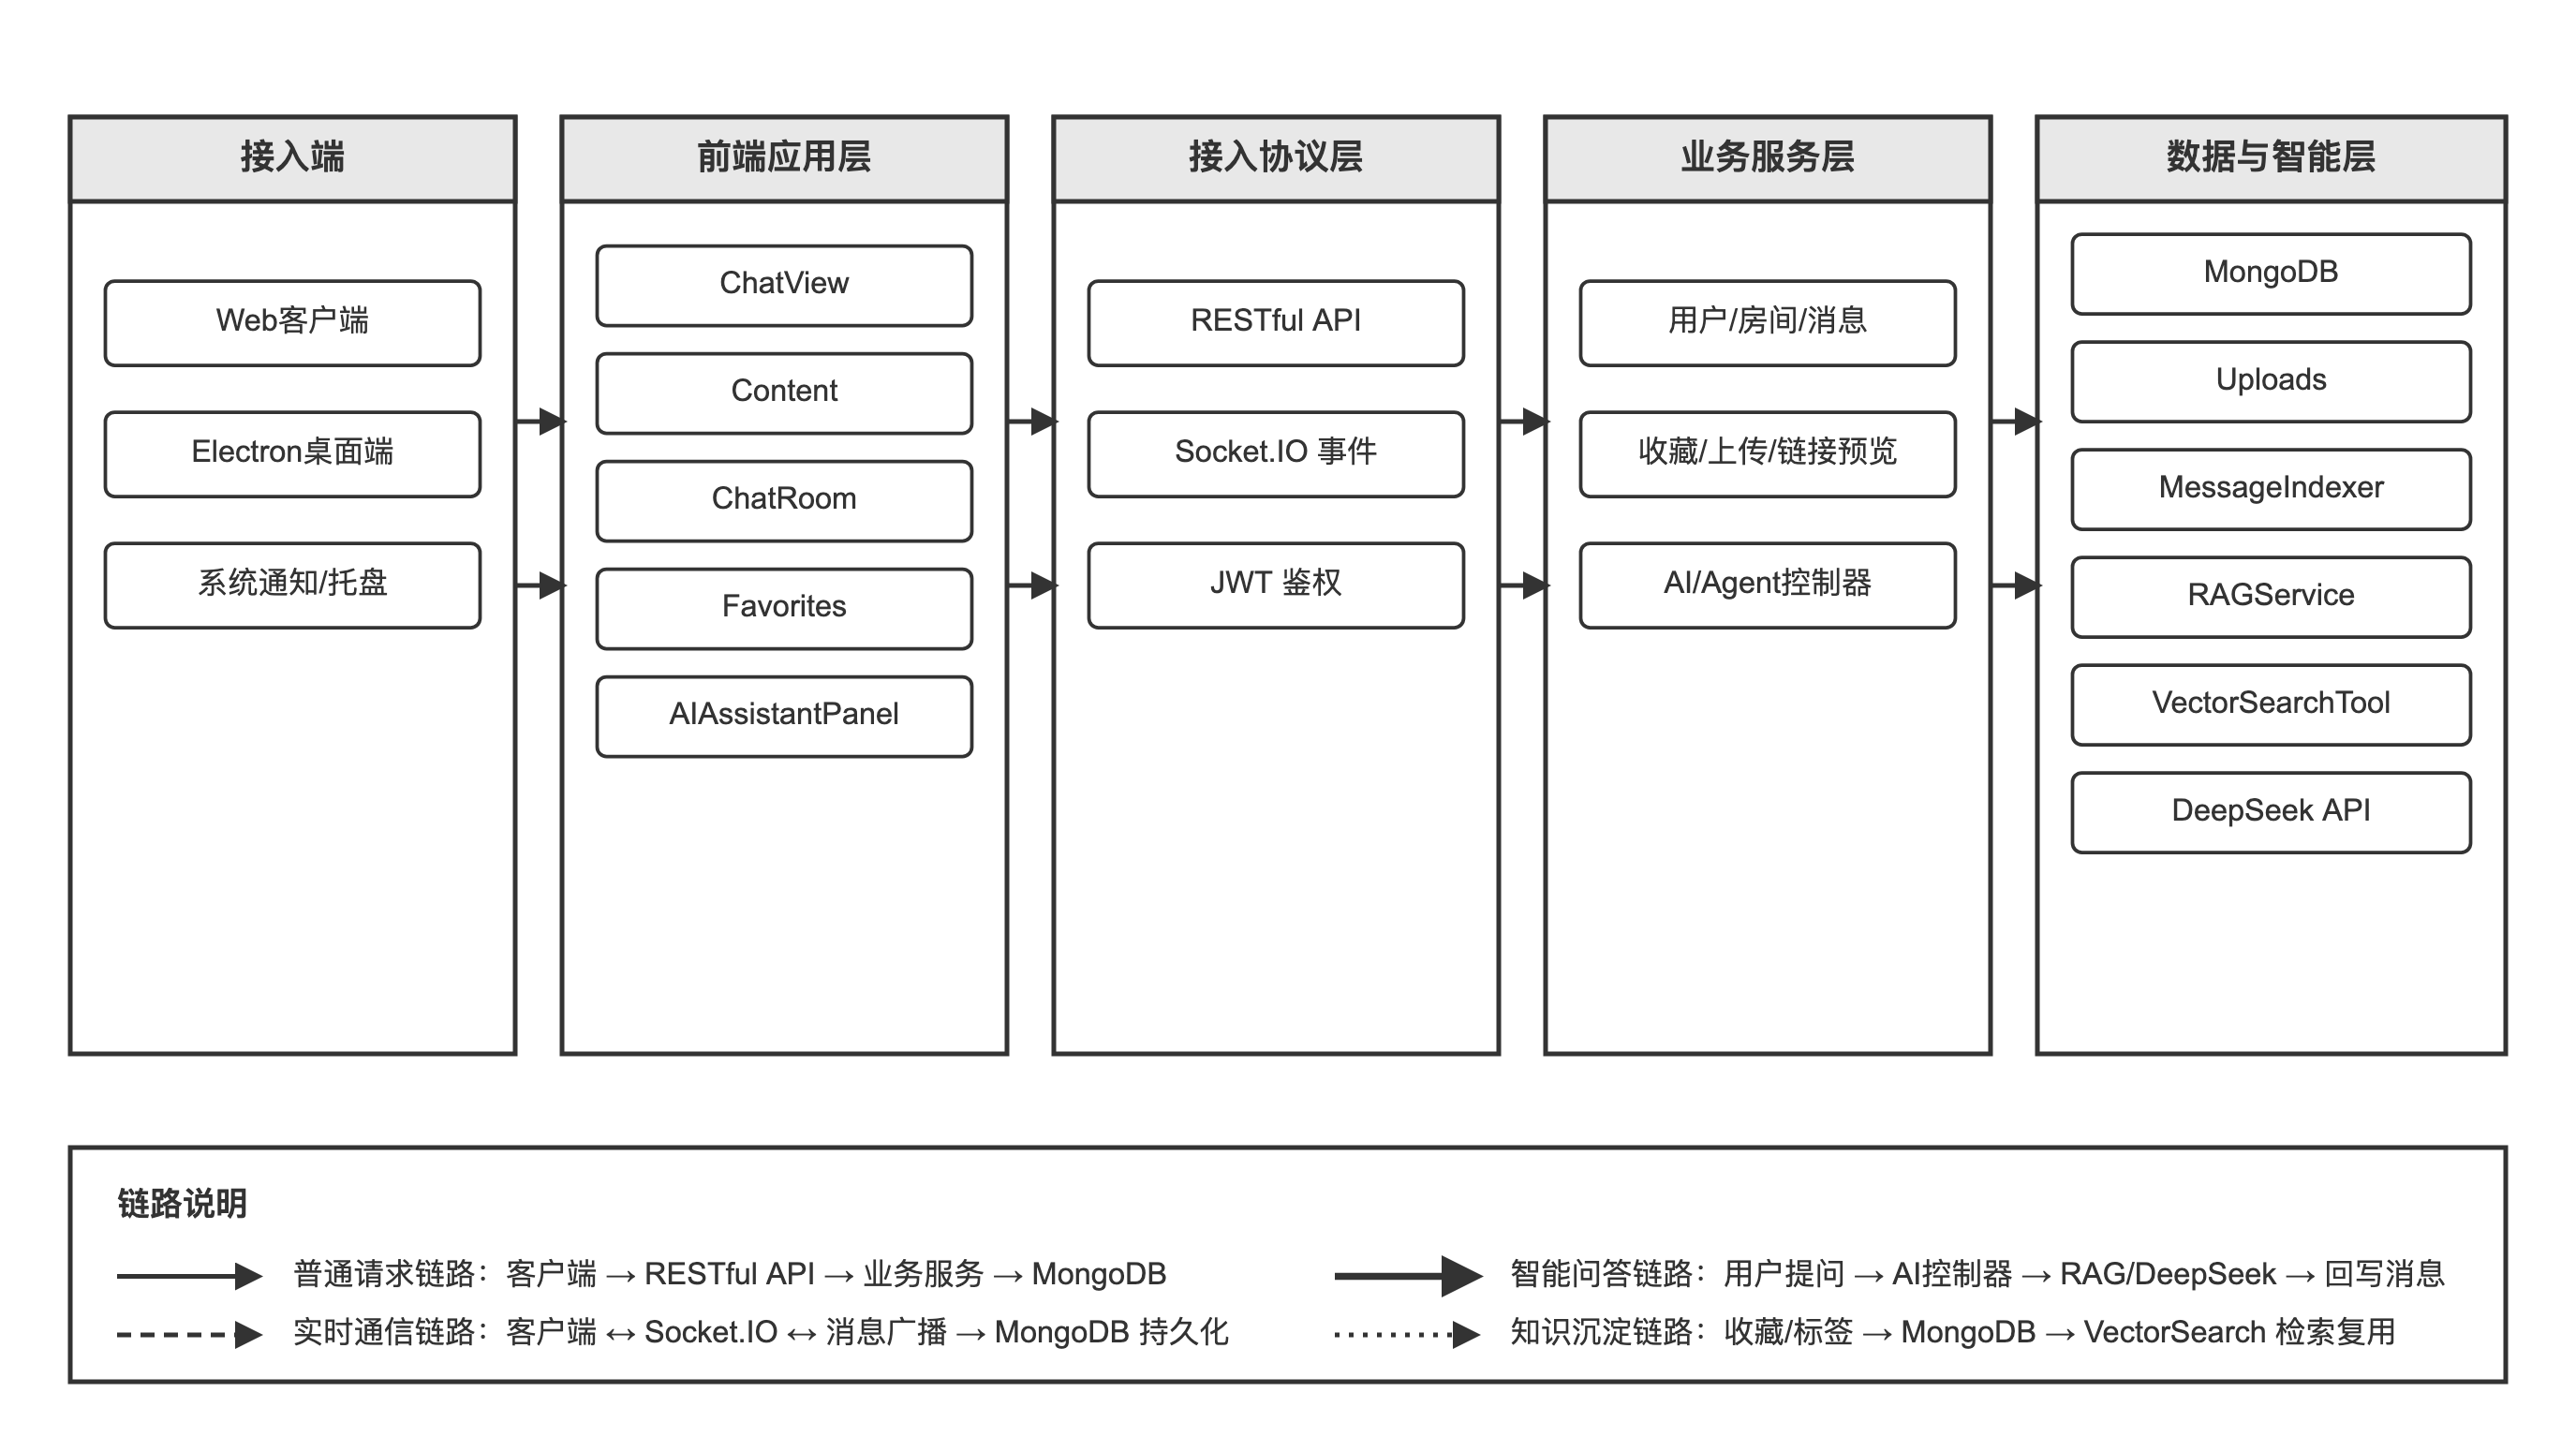
\includegraphics[width=0.82\textwidth,height=0.30\textheight,keepaspectratio]{img/图4_1.png}
\caption{系统架构图}
\label{fig:4-1}
\end{figure}

\FloatBarrier

\subsection{系统总体流程设计}

系统整体运行流程可分为身份认证、会话接入、消息收发、AI 辅助和结果沉淀五个阶段。用户通过邮箱密码或 OAuth2 完成登录后获取 JWT 令牌，再进入指定会话或聊天室发起请求与实时交互。

文本消息和各类附件先由 Express 完成校验与存储，再通过 Socket.IO 同步给相关在线用户。对于聊天室中的技术问题，用户可以调用 AI 助手生成回答，系统会结合当前上下文和检索结果组织提示信息。讨论结束后，用户还可以将摘要或关键代码收藏保存，形成后续复用的资料积累，如图~\ref{fig:4-2}。

\begin{figure}[H]
\centering
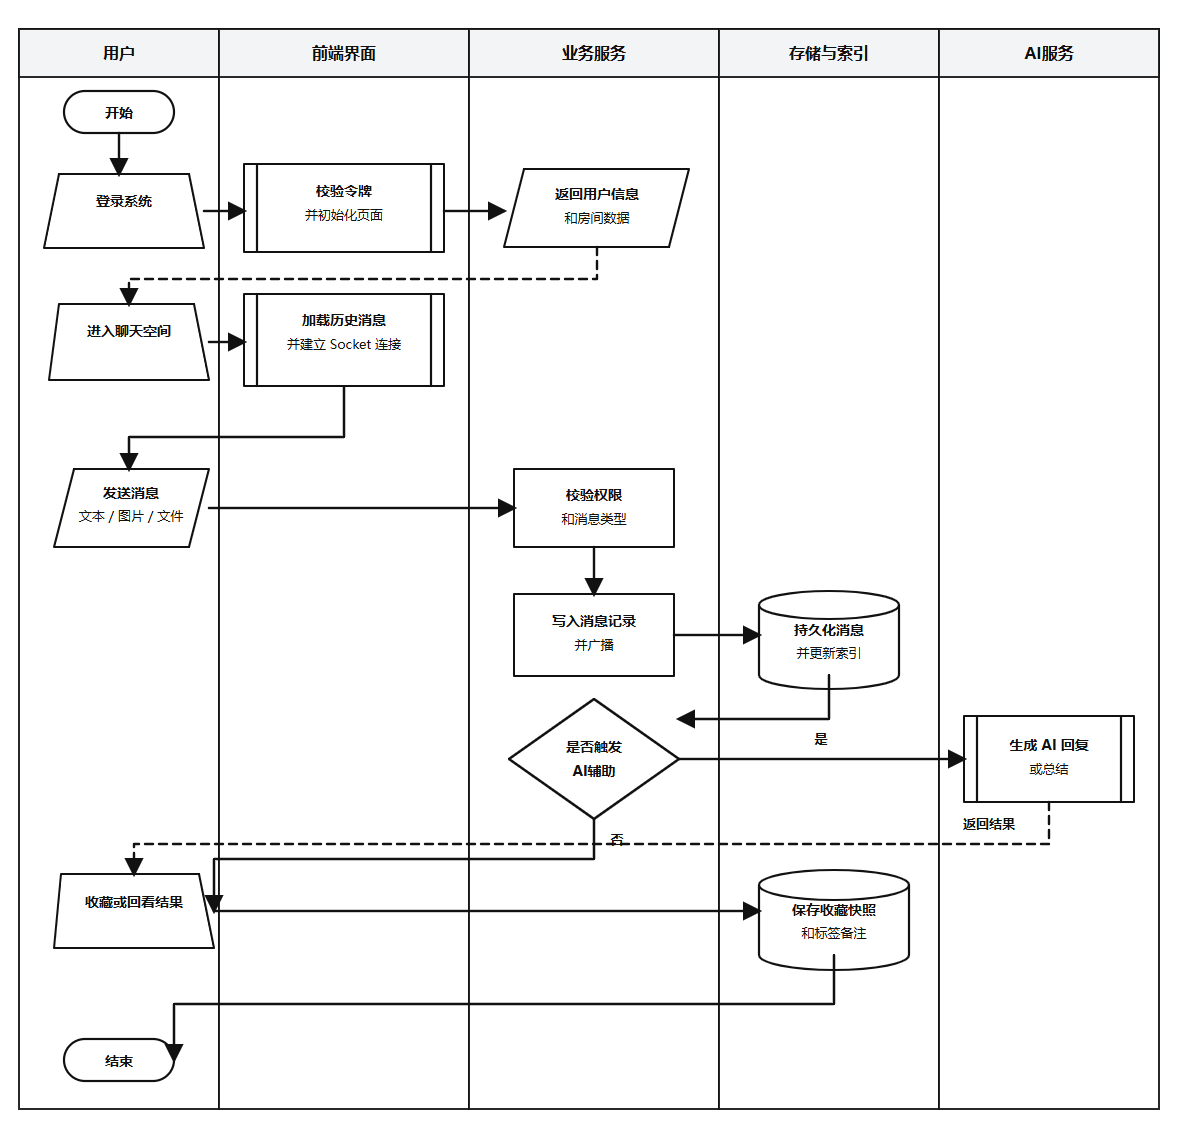
\includegraphics[width=0.94\textwidth,height=0.54\textheight,keepaspectratio]{img/图4_2.png}
\caption{系统总体流程图}
\label{fig:4-2}
\end{figure}

\subsection{系统功能结构设计}

依据业务目标，系统划分为五个核心子模块，包括用户管理、即时通讯、技术聊天室、AI 问答与总结，以及收藏归档。

这种划分便于明确各模块职责，也方便后续在不影响主要业务链路的前提下扩展语音功能或调整大模型接口，系统功能结构见图~\ref{fig:4-3}。

\begin{figure}[H]
\centering
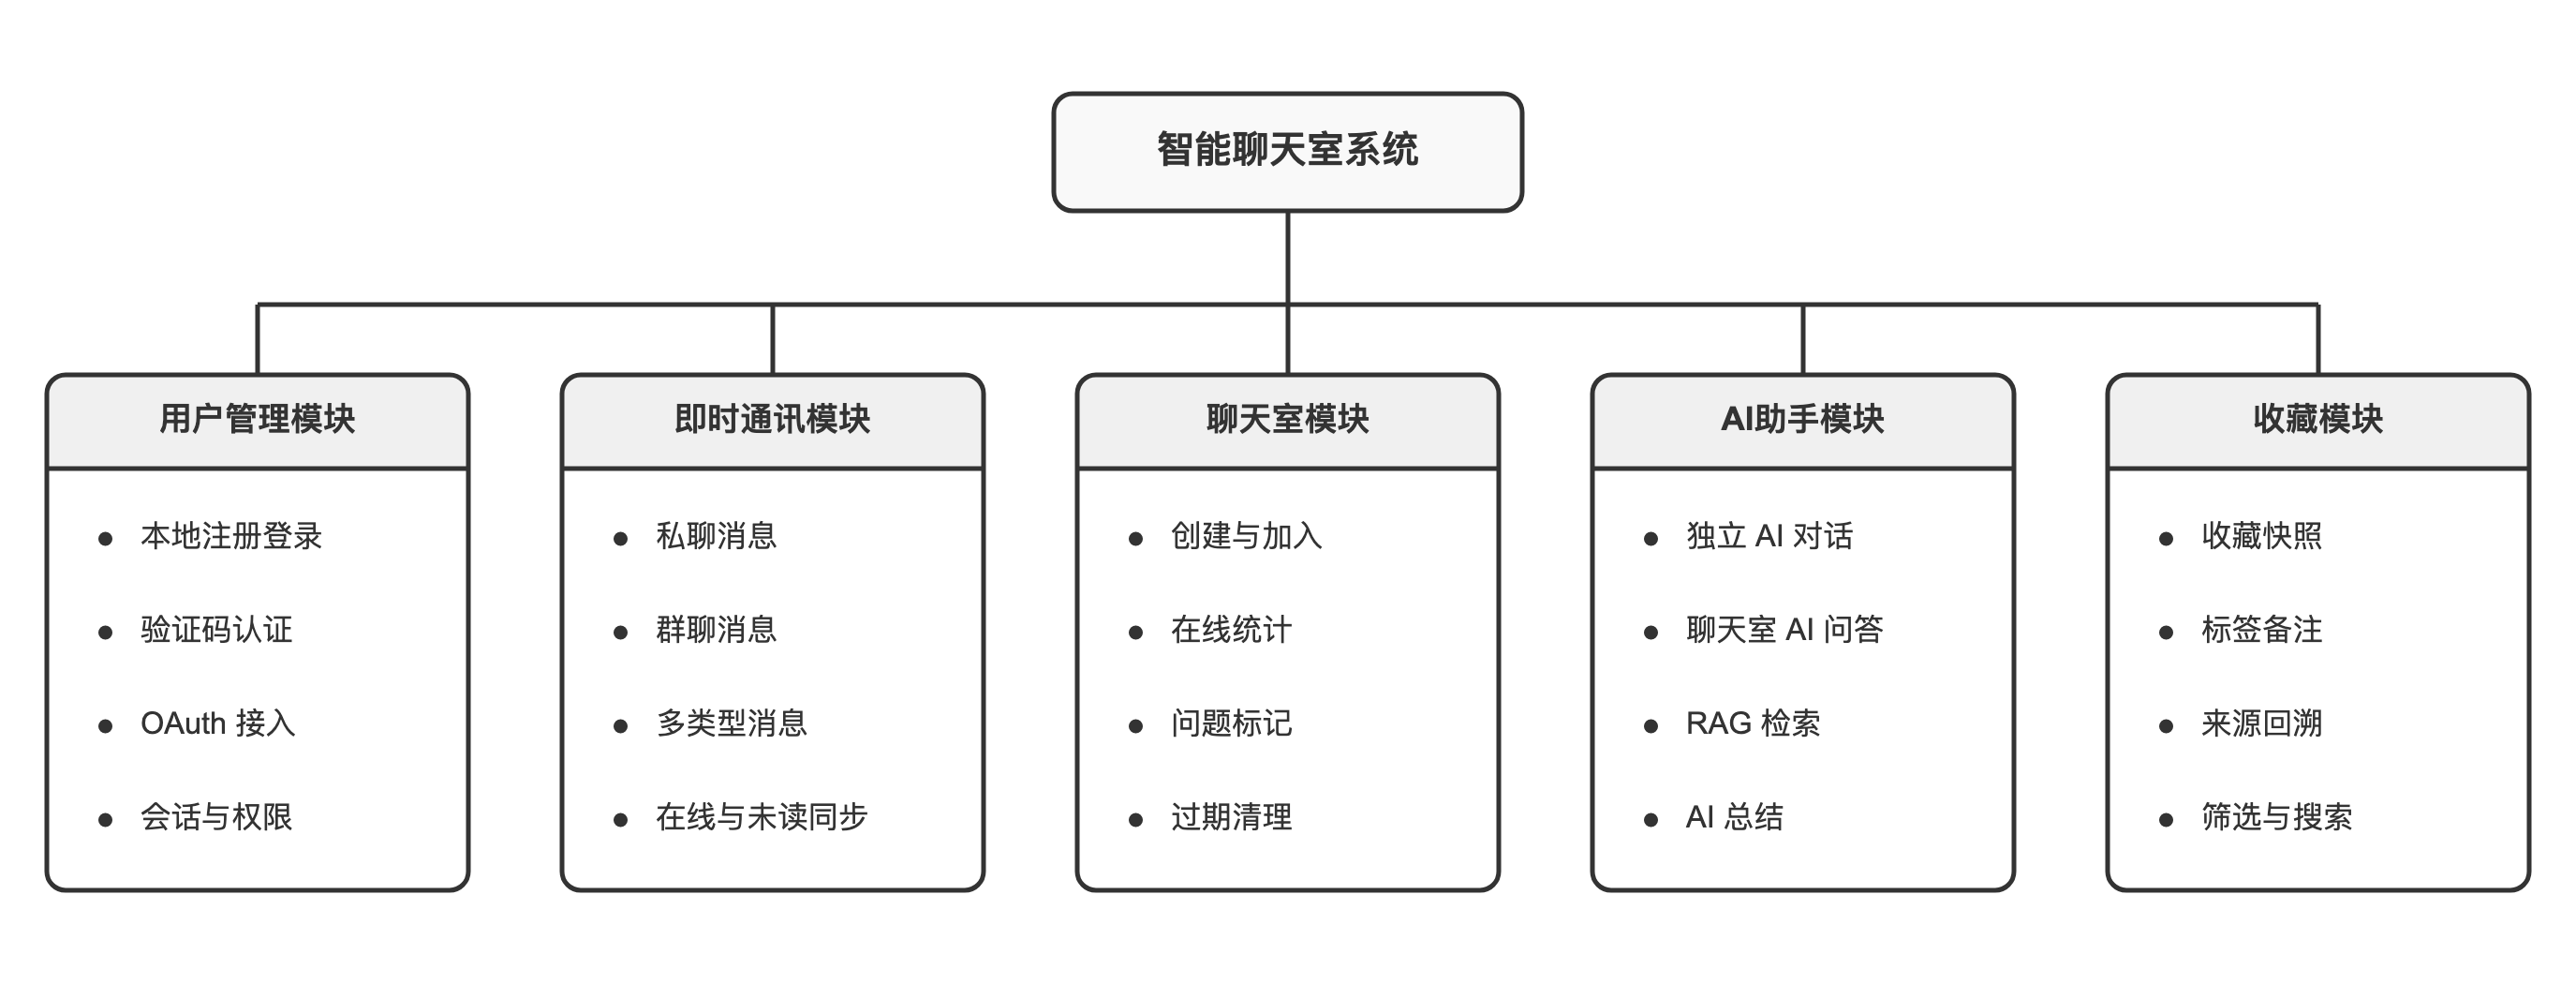
\includegraphics[width=0.95\textwidth, keepaspectratio]{img/图4_3.png}
\caption{系统功能结构图}
\label{fig:4-3}
\end{figure}

\section{功能模块设计}

在总体架构基础上，各功能模块继续按实际业务流程展开。

\subsection{用户管理模块}

用户管理模块负责注册、登录、身份校验和基础资料维护。本地登录流程包括邮箱查重、密码哈希存储和凭证校验，第三方登录则通过 Passport.js 对接 GitHub 和 Google 的 OAuth 授权流程，并在认证成功后返回系统凭证\cite{oauthcn2024,oauthbcp2025}。统一的用户标识会继续用于消息、收藏和聊天室等业务记录，模块内部运作序列如图~\ref{fig:4-4}所示。

\begin{figure}[H]
\centering
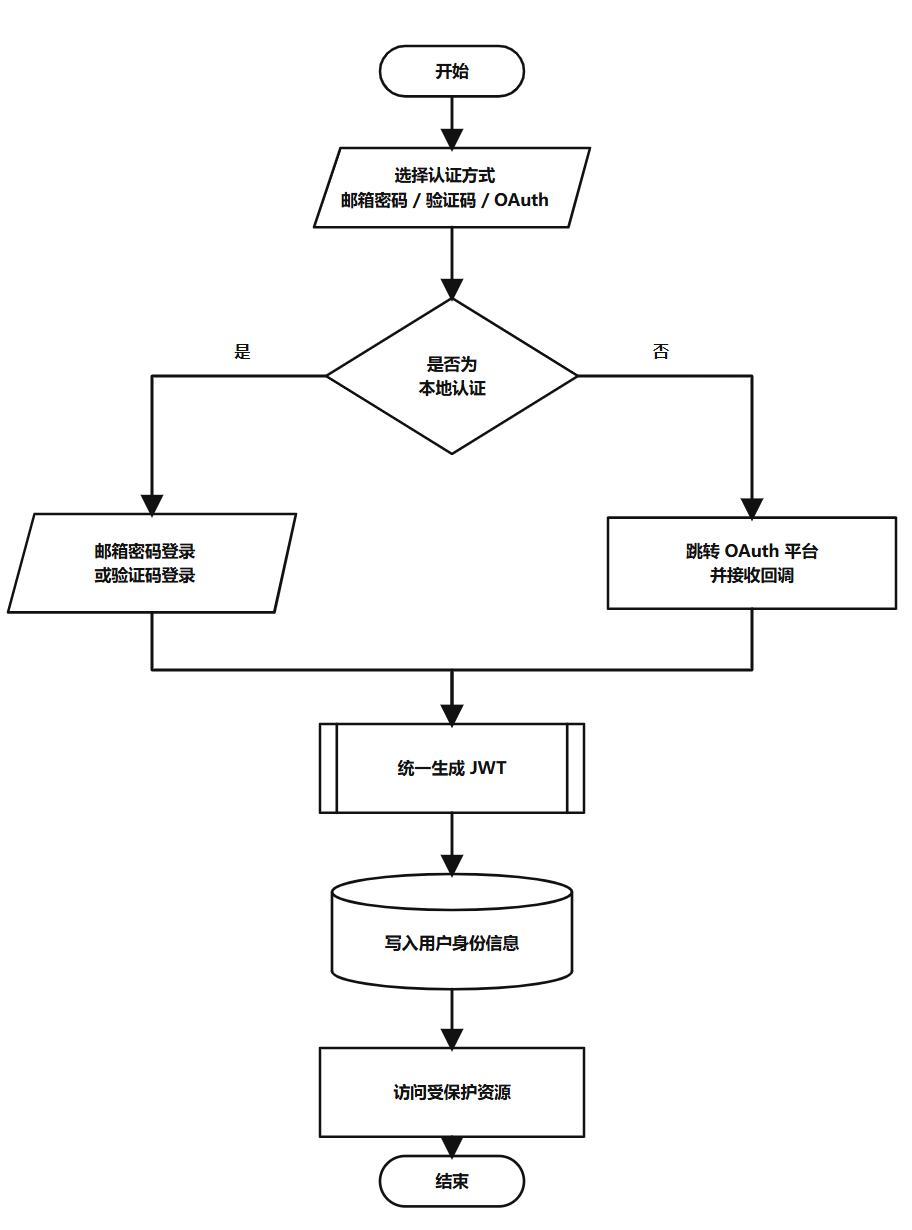
\includegraphics[width=0.94\textwidth,height=0.58\textheight,keepaspectratio]{img/图4_4.png}
\caption{用户模块流程图}
\label{fig:4-4}
\end{figure}

\subsection{即时通讯模块}

即时通讯模块负责私聊与群聊消息的收发和同步。系统将历史消息查询与持久化写入放在 HTTP 接口中，将实时推送交由 WebSocket 处理\cite{socketiodocs2026,imsecurity2024}。消息在写入私聊或群聊数据表后，再通过单播或房间广播分发给在线用户；文本、图片、文件等不同类型的消息也在这一层统一组织后返回前端，流程如图~\ref{fig:4-5}所示。

\begin{figure}[H]
\centering
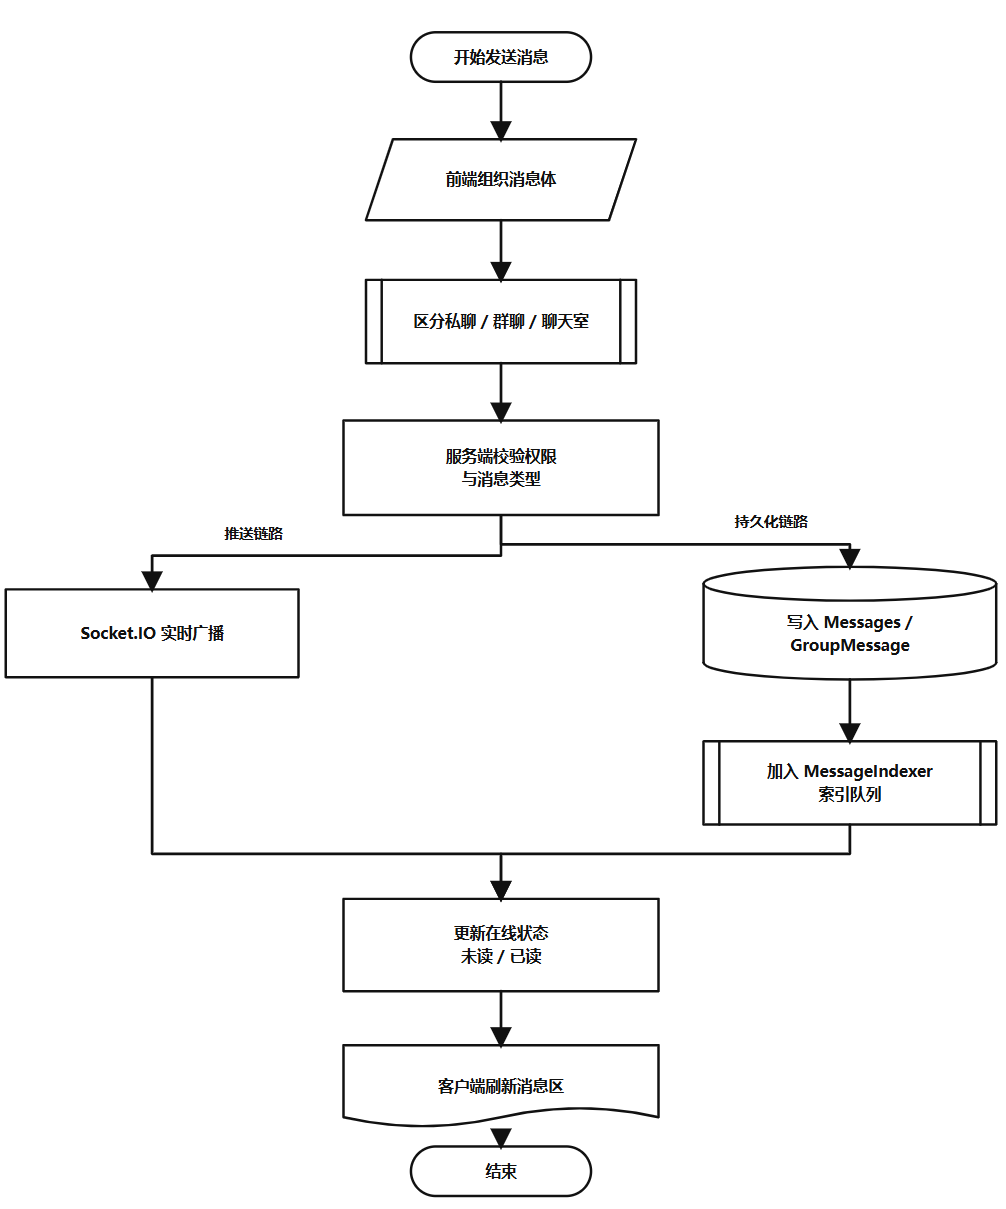
\includegraphics[width=0.94\textwidth,height=0.58\textheight,keepaspectratio]{img/图4_5.png}
\caption{即时通讯流程图}
\label{fig:4-5}
\end{figure}

\subsection{聊天室模块}

聊天室模块面向需要多人实时讨论的技术交流场景。该模块支持公开进入、口令校验或邀请加入等方式，并根据聊天室配置记录有效期与状态变化；当聊天室超期或被解散时，系统会停止新的交互请求并保留历史记录。整体流程如图~\ref{fig:4-6}所示。

\begin{figure}[H]
\centering
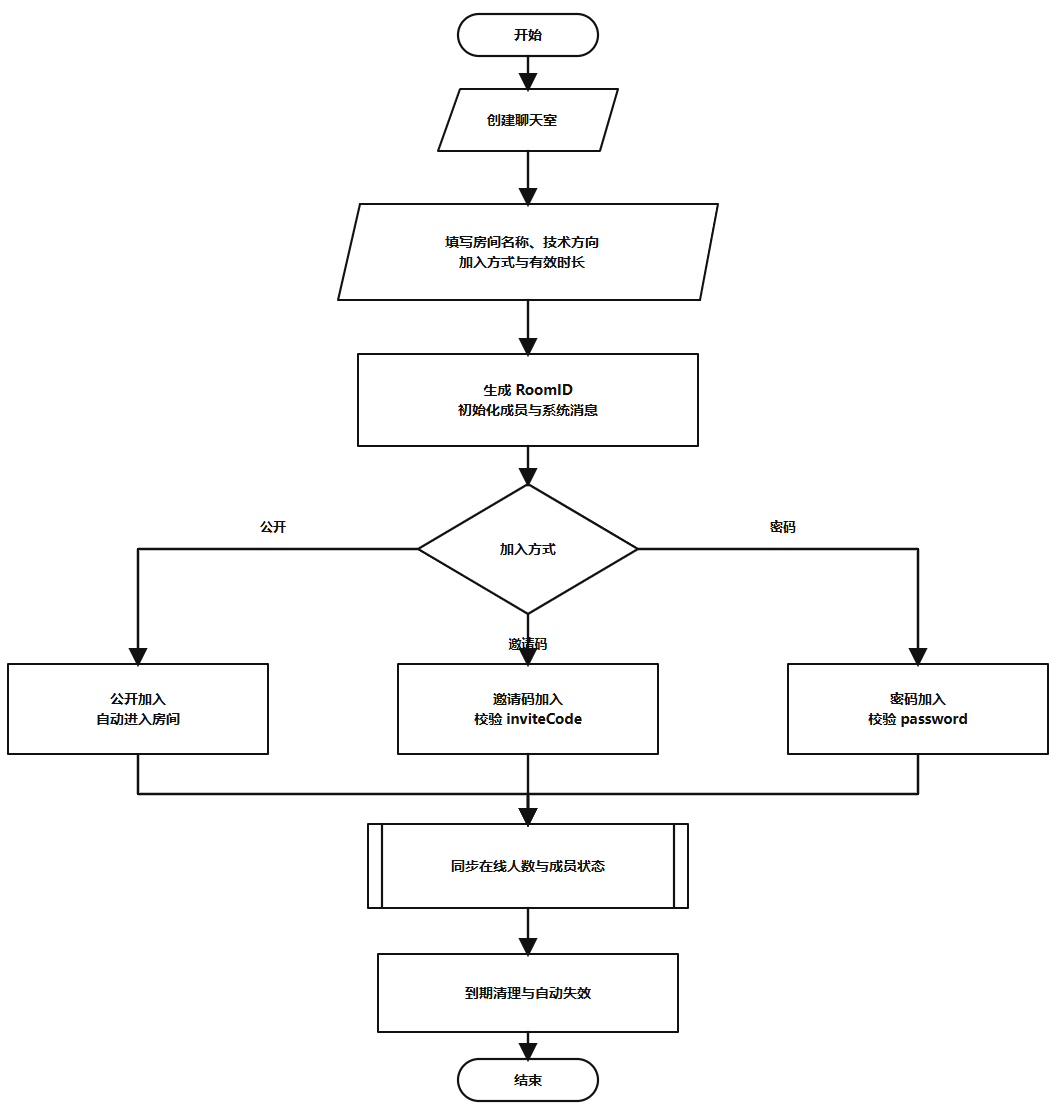
\includegraphics[width=0.94\textwidth,height=0.54\textheight,keepaspectratio]{img/图4_6.png}
\caption{聊天室流程图}
\label{fig:4-6}
\end{figure}

\subsection{AI助手智能问答模块}

AI 助手模块用于在现有聊天链路上提供问答、解释和总结能力。系统在请求模型前会先结合最近消息与检索结果组织上下文，再发起生成请求；返回阶段采用流式输出，并通过 WebSocket 将增量内容同步给房间内其他成员，从而降低等待时长。具体数据组织见图~\ref{fig:4-7}。

\begin{figure}[H]
\centering
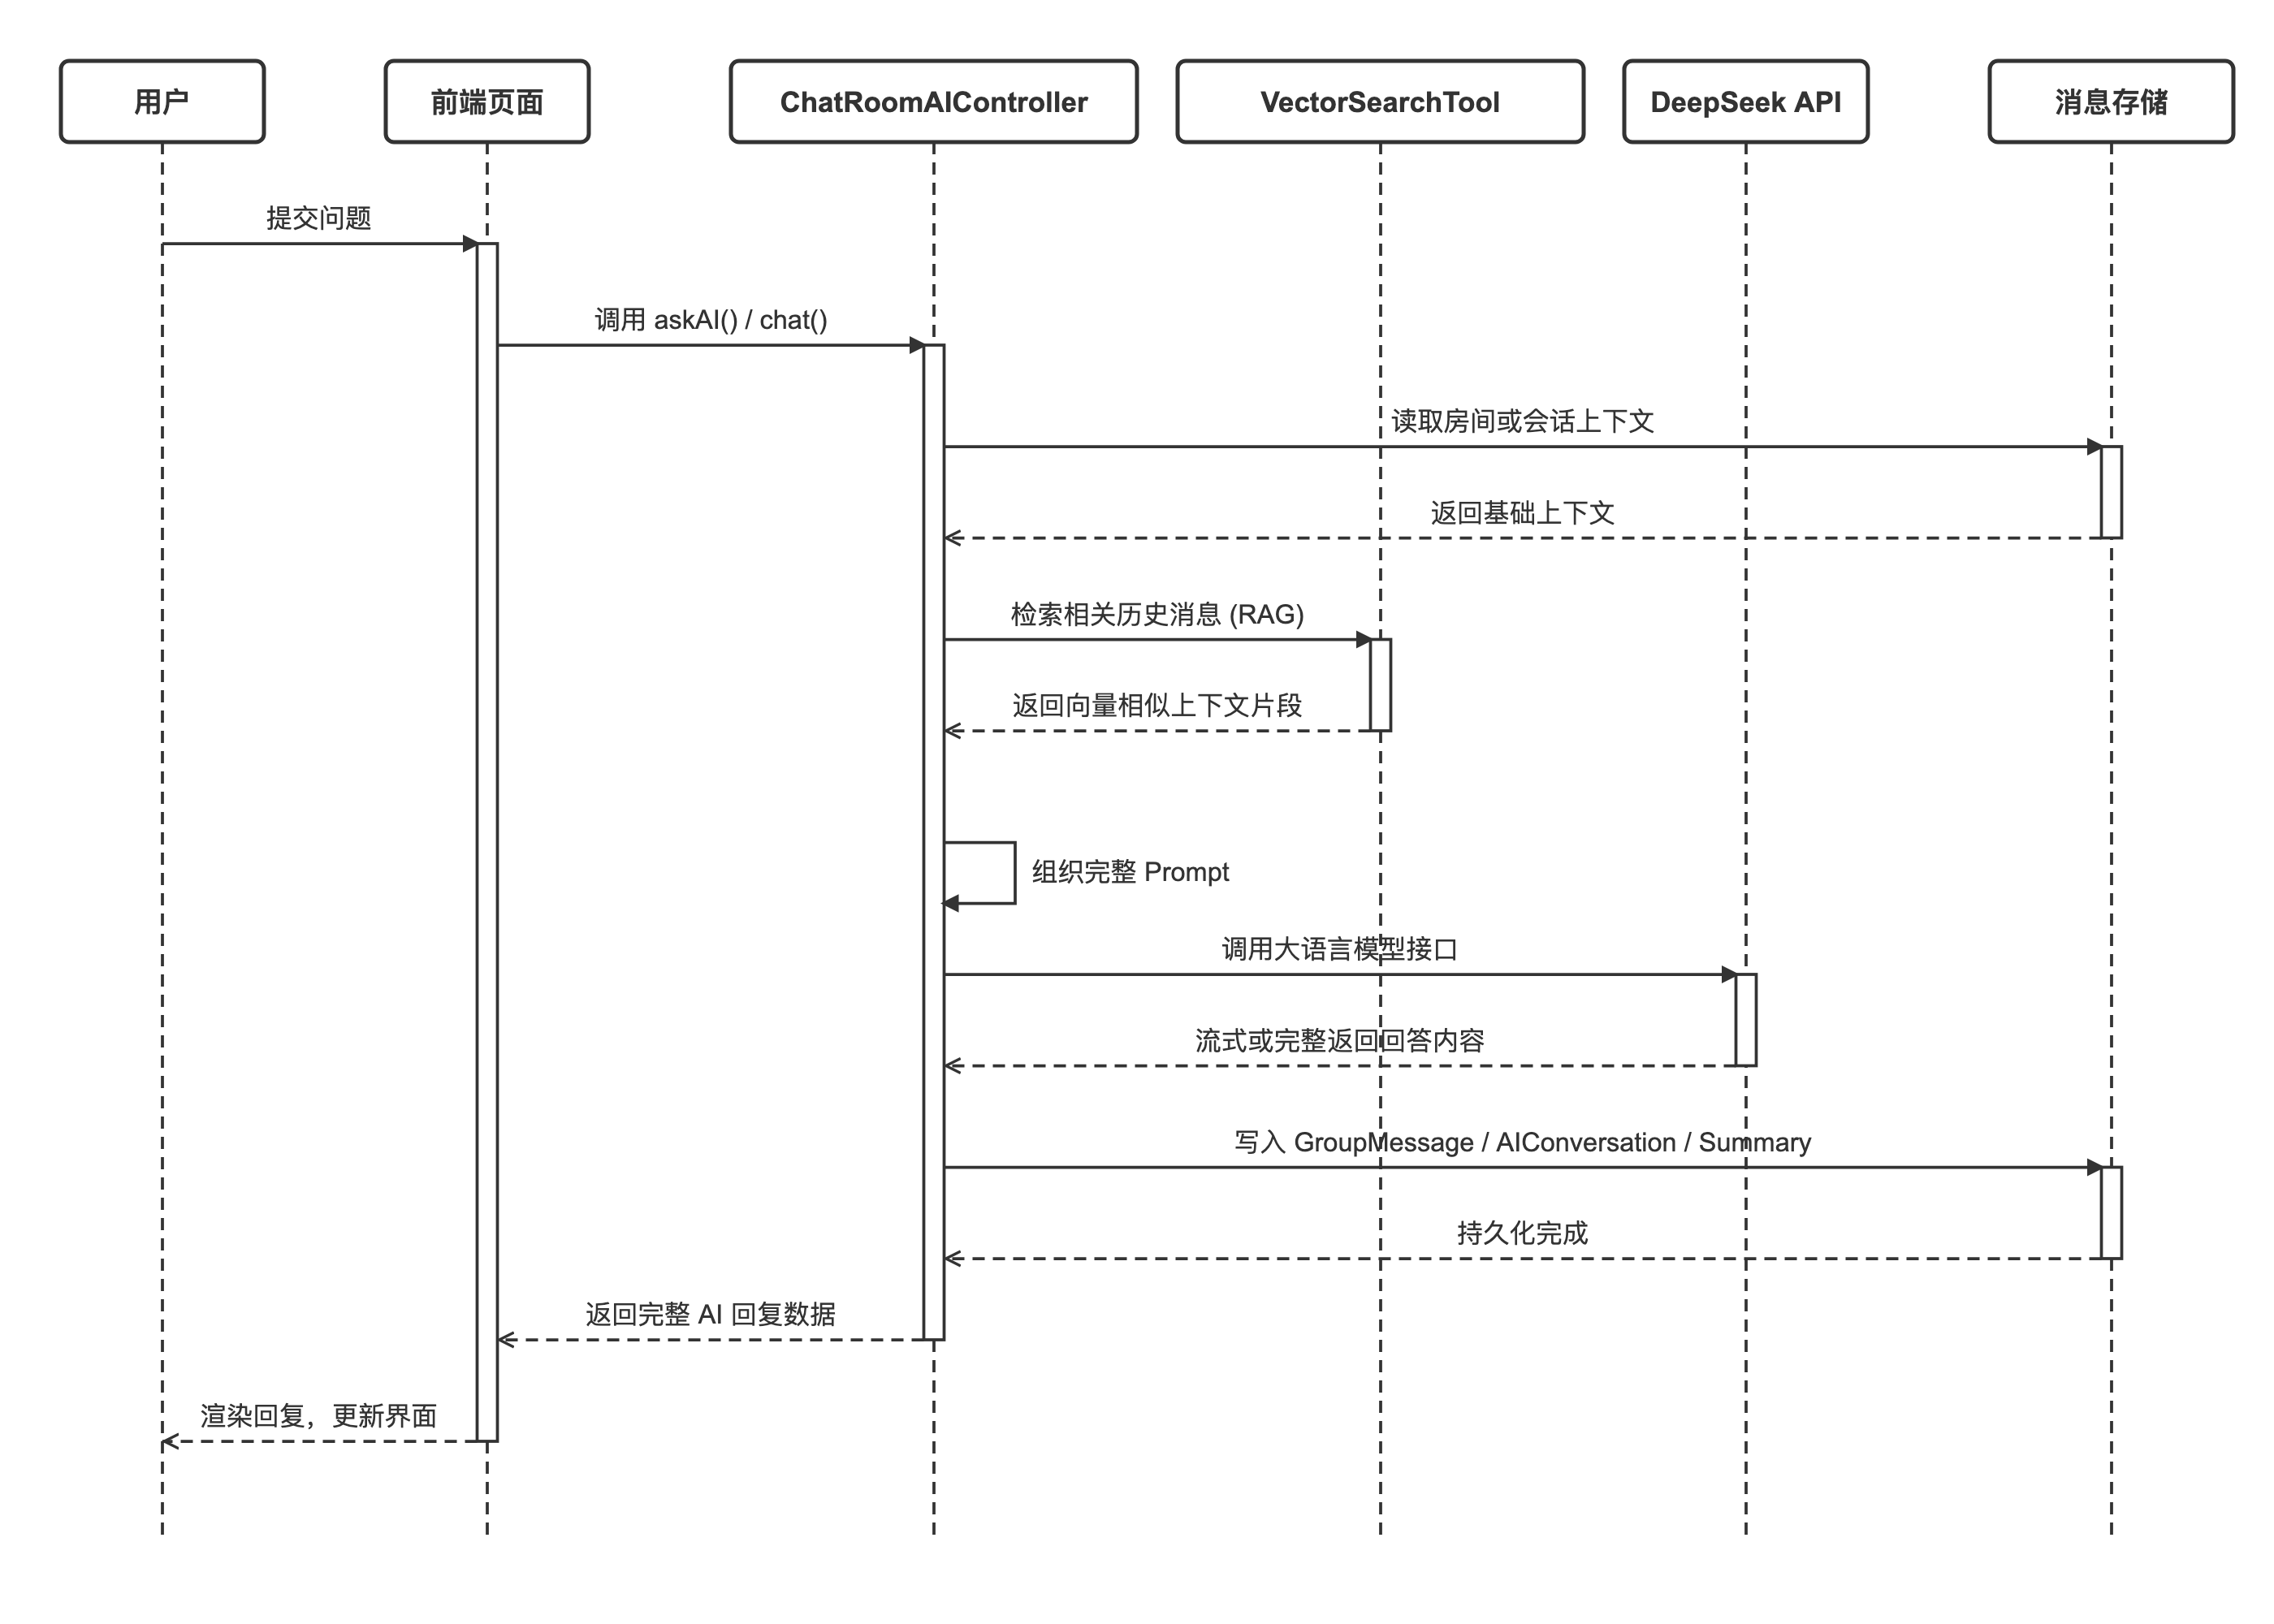
\includegraphics[width=0.94\textwidth,height=0.42\textheight,keepaspectratio]{img/图4_7.png}
\caption{AI助手智能问答模块时序图}
\label{fig:4-7}
\end{figure}

\subsection{收藏模块}

收藏模块用于保存讨论过程中的重要内容。系统在收藏时不仅记录消息标识，还会同步保存消息正文、附件信息和发送者等必要上下文，以便后续独立查看和回溯。用户还可以为收藏内容补充标签和备注，便于检索与整理，交互流程如图~\ref{fig:4-8}。

\begin{figure}[H]
\centering
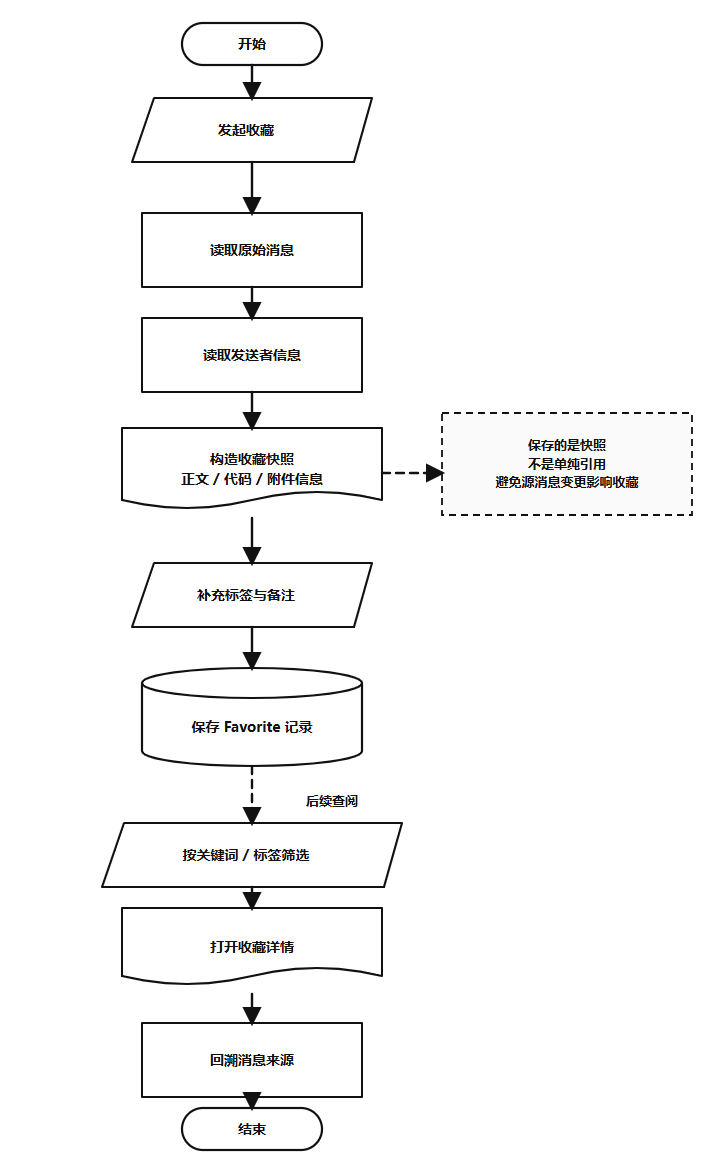
\includegraphics[width=0.94\textwidth,height=0.60\textheight,keepaspectratio]{img/图4_8.png}
\caption{收藏流程图}
\label{fig:4-8}
\end{figure}

\section{界面设计}

界面设计围绕消息阅读、输入操作和状态切换展开，重点保证长时间使用时的信息清晰度与操作连续性。

\subsection{登录与注册界面}
登录与注册界面采用卡片式切换结构，在同一页面中完成登录、注册和 OAuth 登录入口的展示。界面保留必要的表单项和状态提示，减少干扰信息，面板构成见图~\ref{fig:4-9}。

\begin{figure}[H]
\centering
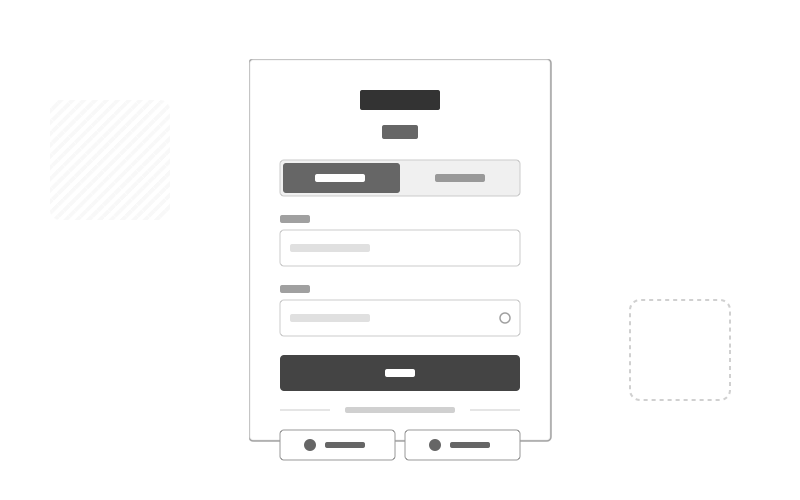
\includegraphics[width=0.88\textwidth,height=0.36\textheight,keepaspectratio]{img/图4_9.png}
\caption{登录与注册界面结构图}
\label{fig:4-9}
\end{figure}

\subsection{主聊天业务界面}
主聊天界面采用左侧导航、中间会话列表、右侧消息详情的三栏布局。该布局能够同时呈现会话切换、消息浏览和当前聊天内容，便于在代码片段、文件和普通文本之间快速切换\cite{vueguide2026,electrondocs2026}，如图~\ref{fig:4-10}所示。

\begin{figure}[H]
\centering
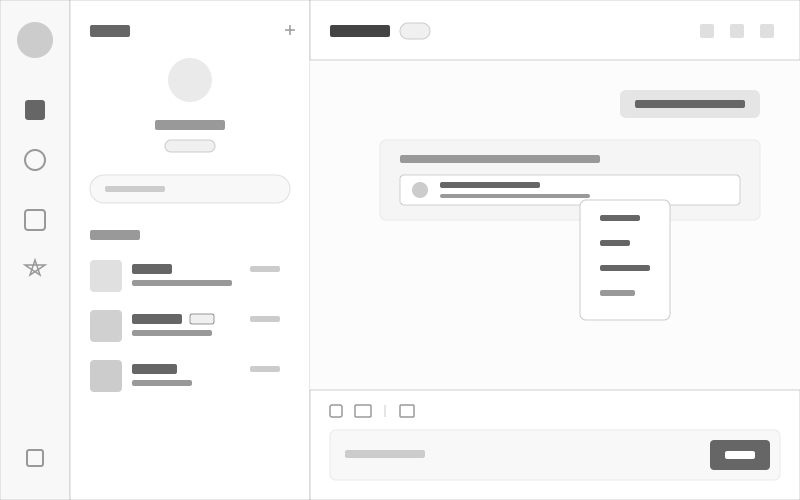
\includegraphics[width=0.88\textwidth,height=0.36\textheight,keepaspectratio]{img/图4_10.png}
\caption{主聊天界面结构图}
\label{fig:4-10}
\end{figure}

\subsection{沉浸式技术聊天室界面}
技术聊天室界面在主聊天布局基础上增加了倒计时、问题状态控制和代码输入辅助等元素，用于突出专题讨论场景。这样可以在多人协作时保持讨论主题集中，并方便用户围绕问题、回答和代码片段进行连续交流，见图~\ref{fig:4-11}。

\begin{figure}[H]
\centering
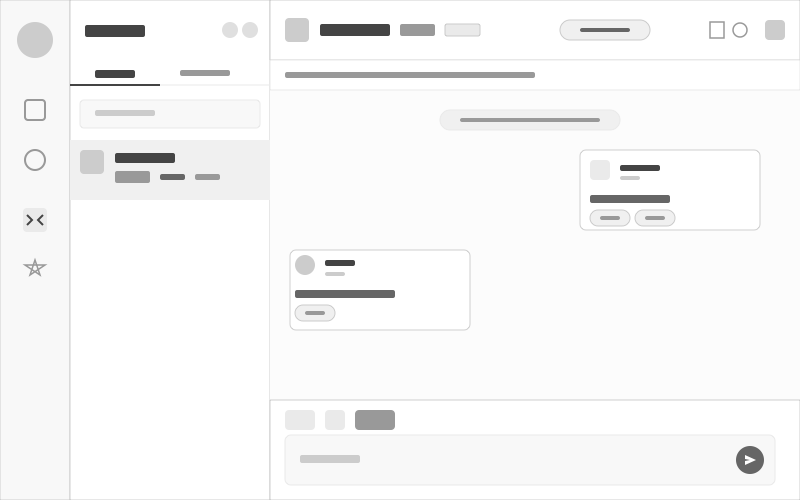
\includegraphics[width=0.88\textwidth,height=0.36\textheight,keepaspectratio]{img/图4_11.png}
\caption{聊天室界面结构图}
\label{fig:4-11}
\end{figure}

\section{数据库设计}

\subsection{E-R图设计}
系统选用 MongoDB 存储用户、房间、消息、收藏和 AI 相关数据，以适应消息类型多样、字段结构变化较快的业务特点。E-R 图以用户、聊天室和消息记录为核心，反映了收藏、AI 对话和总结等数据之间的关联关系，如图~\ref{fig:4-12}所示。

\begin{figure}[H]
\centering
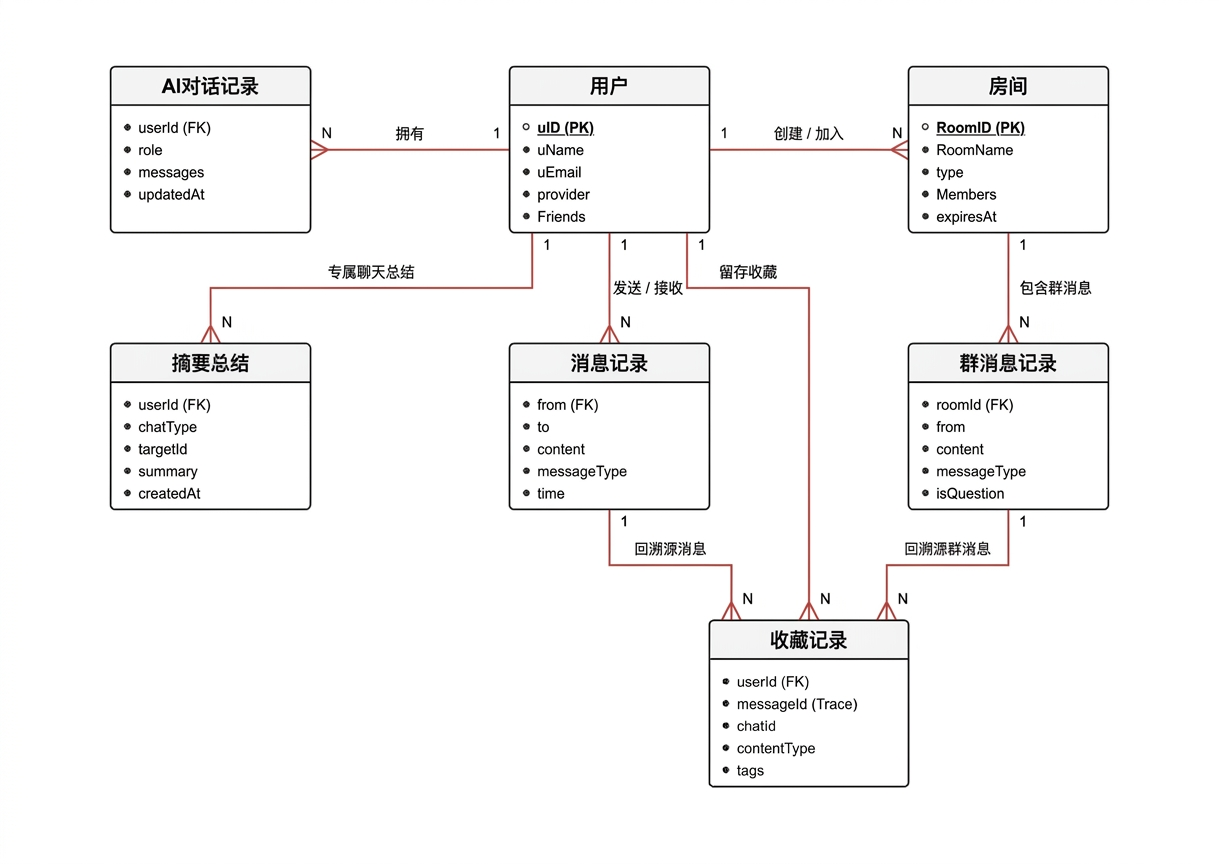
\includegraphics[width=0.88\textwidth,height=0.36\textheight,keepaspectratio]{img/图4_12.png}
\caption{系统数据库E-R图}
\label{fig:4-12}
\end{figure}

\subsection{数据库逻辑结构设计}

数据库逻辑结构设计需要同时考虑消息写入频率、历史查询和扩展字段等需求。基于 MongoDB 的文档模型，系统将核心业务数据拆分为 7 个主要集合，其结构说明如下\cite{mongodbdocs2026}。

\subsubsection{用户表设计}
用户表记录系统认证和身份展示所需的基础信息，如表~\ref{tab:4-1}所示。

\begin{table}[!htbp]
\centering
\caption{用户表结构}
\label{tab:4-1}
\small
\renewcommand{\arraystretch}{1.15}
\setlength{\tabcolsep}{0.6ex}
\begin{tabular}{M{0.17\textwidth}M{0.08\textwidth}M{0.13\textwidth}M{0.10\textwidth}p{0.34\textwidth}}
\toprule
\textbf{字段名} & \textbf{主键} & \textbf{数据类型} & \textbf{是否为空} & \textbf{说明} \\
\midrule
\_id & 是 & ObjectId & 否 & MongoDB 主键 \\
uID & 否 & String & 否 & 业务身份标识编码 \\
uName & 否 & String & 否 & 用户称呼展示 \\
uEmail & 否 & String & 否 & 登录邮箱地址 \\
Password & 否 & String & 是 & 密码哈希值，OAuth 用户可为空 \\
uAvatar & 否 & String & 否 & 用户头像地址 \\
Friends & 否 & Object[] & 是 & 好友列表 \\
googleId / githubId & 否 & String & 是 & 第三方平台用户标识 \\
provider & 否 & String & 否 & 登录来源 \\
\bottomrule
\end{tabular}
\end{table}

\subsubsection{聊天室表设计}
聊天室表用于保存房间基本信息、成员配置和加入方式等内容，如表~\ref{tab:4-2}所示。

\begin{table}[!htbp]
\centering
\caption{聊天室表结构}
\label{tab:4-2}
\small
\renewcommand{\arraystretch}{1.15}
\setlength{\tabcolsep}{0.6ex}
\begin{tabular}{M{0.17\textwidth}M{0.08\textwidth}M{0.13\textwidth}M{0.10\textwidth}p{0.34\textwidth}}
\toprule
\textbf{字段名} & \textbf{主键} & \textbf{数据类型} & \textbf{是否为空} & \textbf{说明} \\
\midrule
\_id & 是 & ObjectId & 否 & 文档主键 \\
\shortstack{RoomID\\RoomName} & 否 & String & 否 & 聊天室编号与名称 \\
\shortstack{Creator\\Admins} & 否 & String[] & 是 & 创建者与管理员列表 \\
Members & 否 & Object[] & 是 & 成员列表及加入时间 \\
type & 否 & String & 否 & 聊天室类型 \\
techDirection & 否 & String & 是 & 技术方向标签 \\
joinType / inviteCode & 否 & String & 是 & 加入方式或邀请码 \\
expiresAt & 否 & Date & 是 & 到期时间 \\
\bottomrule
\end{tabular}
\end{table}

\subsubsection{私聊消息表设计}
私聊消息表用于保存一对一聊天记录及其状态信息，如表~\ref{tab:4-3}所示。

\begin{table}[!htbp]
\centering
\caption{私聊消息表结构}
\label{tab:4-3}
\small
\renewcommand{\arraystretch}{1.15}
\setlength{\tabcolsep}{0.6ex}
\begin{tabular}{M{0.17\textwidth}M{0.08\textwidth}M{0.13\textwidth}M{0.10\textwidth}p{0.34\textwidth}}
\toprule
\textbf{字段名} & \textbf{主键} & \textbf{数据类型} & \textbf{是否为空} & \textbf{说明} \\
\midrule
\_id & 是 & ObjectId & 否 & 文档主键 \\
\shortstack{from\\to} & 否 & String & 否 & 发送方与接收方 \\
time & 否 & Date & 否 & 发送时间 \\
\shortstack{content\\fileInfo} & 否 & Mixed & 是 & 消息内容或附件信息 \\
\shortstack{isRead\\readTime} & 否 & Mixed & 是 & 已读状态与已读时间 \\
\bottomrule
\end{tabular}
\end{table}

\subsubsection{群聊与聊天室消息表设计}
群聊与聊天室消息表用于保存多人会话中的消息内容及互动状态，如表~\ref{tab:4-4}所示。

\begin{table}[!htbp]
\centering
\caption{群聊与聊天室消息表结构}
\label{tab:4-4}
\small
\renewcommand{\arraystretch}{1.15}
\setlength{\tabcolsep}{0.6ex}
\begin{tabular}{M{0.17\textwidth}M{0.08\textwidth}M{0.13\textwidth}M{0.10\textwidth}p{0.34\textwidth}}
\toprule
\textbf{字段名} & \textbf{主键} & \textbf{数据类型} & \textbf{是否为空} & \textbf{说明} \\
\midrule
\shortstack{roomId\\fromName} & 否 & String & 否 & 房间编号与发送者名称 \\
\shortstack{content\\messageType}& 否 & String & 是 & 消息内容与消息类型 \\
\shortstack{codeInfo\\fileInfo} & 否 & Object & 是 & 代码块信息或附件信息 \\
\shortstack{isQuestion\\isSolution}& 否 & Boolean & 否 & 是否为问题或是否标记为解答 \\
\shortstack{reactions\\upvotes} & 否 & Object[] & 是 & 表情反馈与点赞信息 \\
\bottomrule
\end{tabular}
\end{table}

\subsubsection{收藏表设计}
收藏表用于保存用户收藏的消息及其附加说明，如表~\ref{tab:4-5}所示。

\begin{table}[!htbp]
\centering
\caption{收藏表结构}
\label{tab:4-5}
\small
\renewcommand{\arraystretch}{1.15}
\setlength{\tabcolsep}{0.6ex}
\begin{tabular}{M{0.17\textwidth}M{0.08\textwidth}M{0.13\textwidth}M{0.10\textwidth}p{0.34\textwidth}}
\toprule
\textbf{字段名} & \textbf{主键} & \textbf{数据类型} & \textbf{是否为空} & \textbf{说明} \\
\midrule
\shortstack{userId\\messageId} & 否 & String & 否 & 收藏用户与来源消息 \\
\shortstack{chatId\\contentType} & 否 & String & 否 & 所属会话与内容类型 \\
\shortstack{content\\codeInfo} & 否 & Mixed & 是 & 收藏正文与代码信息快照 \\
\shortstack{tags\\note} & 否 & Mixed & 是 & 自定义标签与备注 \\
\bottomrule
\end{tabular}
\end{table}

\subsubsection{AI对话表设计}
AI 对话表用于保存用户与 AI 助手之间的历史对话，如表~\ref{tab:4-6}所示。

\begin{table}[!htbp]
\centering
\caption{AI对话表结构}
\label{tab:4-6}
\small
\renewcommand{\arraystretch}{1.15}
\setlength{\tabcolsep}{0.6ex}
\begin{tabular}{M{0.17\textwidth}M{0.08\textwidth}M{0.13\textwidth}M{0.10\textwidth}p{0.34\textwidth}}
\toprule
\textbf{字段名} & \textbf{主键} & \textbf{数据类型} & \textbf{是否为空} & \textbf{说明} \\
\midrule
\shortstack{userId\\role} & 否 & String & 否 & 所属用户与角色类型 \\
rolePrompt & 否 & String & 是 & 角色提示词 \\
messages & 否 & Object[] & 是 & 对话消息列表 \\
\bottomrule
\end{tabular}
\end{table}

\subsubsection{聊天总结表设计}
聊天总结表用于保存会话的阶段总结结果及相关统计信息，如表~\ref{tab:4-7}所示。

\begin{table}[!htbp]
\centering
\caption{聊天总结表结构}
\label{tab:4-7}
\small
\renewcommand{\arraystretch}{1.15}
\setlength{\tabcolsep}{0.6ex}
\begin{tabular}{M{0.17\textwidth}M{0.08\textwidth}M{0.13\textwidth}M{0.10\textwidth}p{0.34\textwidth}}
\toprule
\textbf{字段名} & \textbf{主键} & \textbf{数据类型} & \textbf{是否为空} & \textbf{说明} \\
\midrule
\shortstack{targetId\\chatType} & 否 & String & 否 & 总结对象编号与会话类型 \\
summary & 否 & Object & 否 & 总结结果对象 \\
\shortstack{statistics\\msgCount} & 否 & Mixed & 是 & 统计信息与消息数量 \\
\bottomrule
\end{tabular}
\end{table}

\section{核心底层机制与部署拓扑设计}

\subsection{WebSocket 即时通信协作机理}

系统使用 WebSocket 处理消息实时分发和房间状态同步。服务端在消息写入或状态变更后向对应用户或房间广播事件，客户端接收事件后再更新消息列表、未读状态和界面显示，从而保证实时通信与持久化数据保持一致，具体机理如图~\ref{fig:4-13}所示。

\begin{figure}[H]
\centering
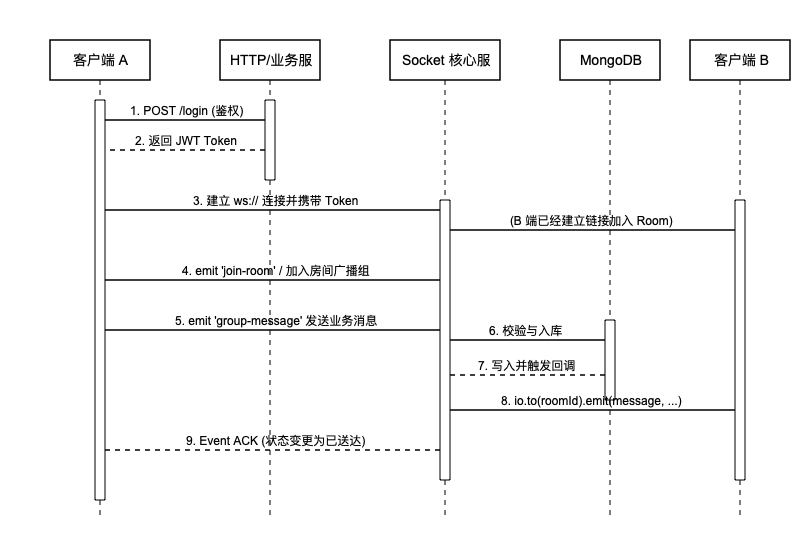
\includegraphics[width=0.94\textwidth,height=0.42\textheight,keepaspectratio]{img/图4_13.png}
\caption{Socket即时通信底层时序图}
\label{fig:4-13}
\end{figure}

\subsection{系统物理部署与网络拓扑架构}

在物理部署上，Nginx 负责统一接收外部请求并转发到 Express 与 Socket.IO 服务，MongoDB 用于保存用户、消息和收藏等业务数据，DeepSeek 模型服务负责处理需要生成能力的请求，整体网络拓扑如图~\ref{fig:4-14}所示。

\begin{figure}[H]
\centering
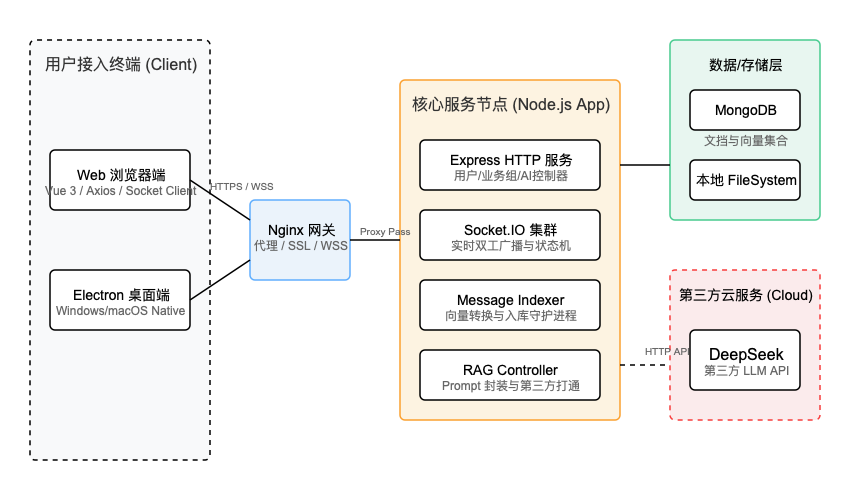
\includegraphics[width=0.90\textwidth, keepaspectratio]{img/图4_14.png}
\caption{系统物理部署与网络拓扑架构图}
\label{fig:4-14}
\end{figure}

从部署关系看，Web 端与桌面端共享同一套后端服务入口，实时通信、历史索引与 AI 能力围绕业务服务层统一组织。

\chapter{系统实现}

\newcommand{\chapterfiveplaceholder}[1]{%
\begin{center}
\fbox{\parbox[c][4.0cm][c]{0.82\textwidth}{\centering #1（占位）}}
\end{center}
\begin{center}
#1（占位）
\end{center}
}
\newcommand{\thesiscirclednum}[1]{\ding{\numexpr191+#1\relax}}
\newcommand{\thesisdescitem}[3]{%
\par\addvspace{0.55\baselineskip}%
\noindent\hspace*{2em}\thesiscirclednum{#1}\ #2\par
\vspace{0.1\baselineskip}%
\noindent\hspace*{2em}#3\par
}
\newcommand{\thesisparenitem}[3]{%
\par\addvspace{0.55\baselineskip}%
\noindent\hspace*{2em}（#1）\ #2\par
\vspace{0.1\baselineskip}%
\noindent\hspace*{2em}#3\par
}

\tikzset{
  chapterfivebox/.style={rectangle, draw, rounded corners=2pt, minimum width=3.7cm, minimum height=0.9cm, text centered, align=center},
  chapterfivedecision/.style={diamond, draw, minimum width=2.8cm, minimum height=1.0cm, text centered, aspect=2},
  chapterfivearrow/.style={->, >=Stealth, thick}
}

本章主要介绍系统的实际实现。前文已经完成需求分析和总体设计，这一章转向具体落地，重点说明后端、Web 前端和桌面端分别如何实现核心功能。本系统后端负责鉴权、消息存储、AI 调用和 Socket.IO 实时通信，前端负责聊天界面、状态同步、桌面端托盘和通知交互\cite{expressdocs2026,socketiodocs2026,electrondocs2026}。下面按后端、Web 前端和桌面端三个部分展开说明。

\section{后端实现}

\subsection{后端项目结构说明}

本系统后端由主入口文件统一完成服务启动和基础配置加载，具体业务再按职责拆分到路由、控制器、模型、Socket 事件、AI 代理和服务模块中。这样可以避免单个文件承担过多逻辑，也方便后续扩展接口、调整数据模型和排查实时通信问题。整体上，后端核心内容可以概括为配置层、路由层、控制器层、数据模型层、实时通信层以及 AI 服务与工具层。

\thesisparenitem{1}{\texttt{config}}{主要处理数据库连接和 OAuth 配置。MongoDB 连接在数据库配置文件中完成，Google、GitHub 登录策略则在第三方登陆中注册。}
\thesisparenitem{2}{\texttt{routes}}{负责把请求路径分配给不同业务模块。用户、私聊、聊天室、AI、收藏和上传接口都在这一层挂接。}
\thesisparenitem{3}{\texttt{controllers}}{负责具体业务逻辑。前端发起的登录、消息发送和历史记录读取等请求，最终都会在这一层完成处理。}
\thesisparenitem{4}{\texttt{models}}{对应 MongoDB 文档结构。系统把私聊消息和群聊消息分开建模，和前端界面的功能划分保持一致。}
\thesisparenitem{5}{\texttt{middlewares}}{中间件中中较关键的是验证模块，它负责 JWT 校验，用于控制受保护接口的访问。}
\thesisparenitem{6}{\texttt{sockets}}{负责 Socket.IO 事件。私聊、群聊、语音房间和代码协作分别独立放置，便于按功能定位实时通信问题。}
\thesisparenitem{7}{\texttt{agents}、\texttt{services} 和 \texttt{tools}}{一起组成 AI 能力。这一部分不是简单封装模型调用，而是实现了带有步骤编排的 Agent 结构。}

本项目设计的这套拆分方式已经能够覆盖当前聊天系统的核心需求。后续如果继续增加消息审核、AI 角色管理或者更细的权限控制，也可以沿着这套结构继续扩展，不会混淆旧代码。

\subsection{核心模块实现}

\subsubsection{用户模块}

本系统的用户模块支持邮箱密码登录、邮箱验证码登录、邮箱注册，以及 Google、GitHub 的 OAuth 登录。实现上，用户认证、路由分发和第三方登录配置分别落在对应模块中。登录成功以后，系统返回 JWT，前端再把 token 和用户信息保存到本地，并继续初始化 Socket 连接和在线状态\cite{oauthcn2024,oauthbcp2025}。

用户登录成功后，系统会统一生成带有效期的 JWT，并在响应中同时返回用户标识、昵称、邮箱与头像等基础资料，方便前端一次完成身份保持、用户信息回填和 Socket 初始化。

用户认证模块围绕统一身份体系展开。普通注册时，后端会先校验邮箱格式和密码强度，再使用 \texttt{bcrypt} 对密码进行哈希；普通登录时，则根据邮箱查询用户并比对哈希结果，验证通过后再生成 token。验证码登录流程先通过邮件服务生成并暂存验证码，用户提交后再完成核验。OAuth 登录需要先从第三方平台获取用户资料，再根据第三方 ID 或邮箱匹配本地账户，未匹配到时自动创建新账户。该设计使不同登录方式可以共用同一套用户数据。

后端在 \texttt{/api/user/info} 用户信息接口中统一返回当前用户的基础信息。前端在登录完成后通过该接口补齐头像和邮箱，设置页修改资料后也会再次请求该接口；OAuth 回调完成后，前端同样会先读取当前用户信息，再决定后续页面跳转。因此，用户模块不仅承担登录和注册功能，也为其他页面提供统一的身份基础。

邮箱密码登录与 JWT 下发的相关实现见附录A。

\subsubsection{聊天模块}

本系统的聊天模块分成私聊和群聊两条主线。私聊围绕一对一消息收发与历史查询展开，群聊和技术聊天室则同时支持多人讨论、问题标记和协作交流。除最基础的文本消息外，系统还支持图片、文件、语音、代码片段、引用回复和问题标记。

群聊消息在进入数据库前会先补齐发送者昵称、头像、消息类型和引用信息等字段，写库完成后再更新房间活跃时间，并通过房间广播把完整消息对象同步给在线成员。

群聊消息发送时，后端会先确认房间是否存在以及当前用户是否为成员，再补齐发送者昵称和头像，最后将消息写入群消息集合。其中，群消息文档会冗余保存 \texttt{fromName} 和 \texttt{fromAvatar}，从而避免前端在加载历史消息时逐条查询用户表。私聊部分采用相近思路，但数据结构相对更简洁，核心字段主要包括 \texttt{from}、\texttt{to}、\texttt{content} 和 \texttt{isRead}。

从数据模型设计看，群聊并不等同于简单的多人私聊。群消息模型中额外定义了 \texttt{quotedMessage}、\texttt{isQuestion}、\texttt{questionStatus}、\texttt{isSolution}、\texttt{reactions} 等字段，用于对应前端的技术讨论功能。例如，用户在聊天室中标记问题、设置最佳答案或添加表情反应时，相关状态都会写入消息文档，而不是仅停留在界面层。这样一来，聊天室中的问题追踪与讨论辅助功能就有了明确的数据模型支撑。

私聊消息查询与发送、技术聊天室创建等相关实现分别见附录B与附录C。

\subsubsection{AI智能检索与流式交互（RAG \& SSE）}

本系统的 AI 模块将ai流式对话接口设计为结合 RAG 向量检索与 Server-Sent Events (SSE) 的流式处理接口。当用户在聊天室中发送带有 \texttt{@AI} 的问题时，系统不会直接把请求转发给模型，而是先整理当前房间的上下文，再调用模型生成回答\cite{qaoverview2025,ragllmsurvey2024,ragsurveycn2025}。

\begin{figure}[H]
\centering
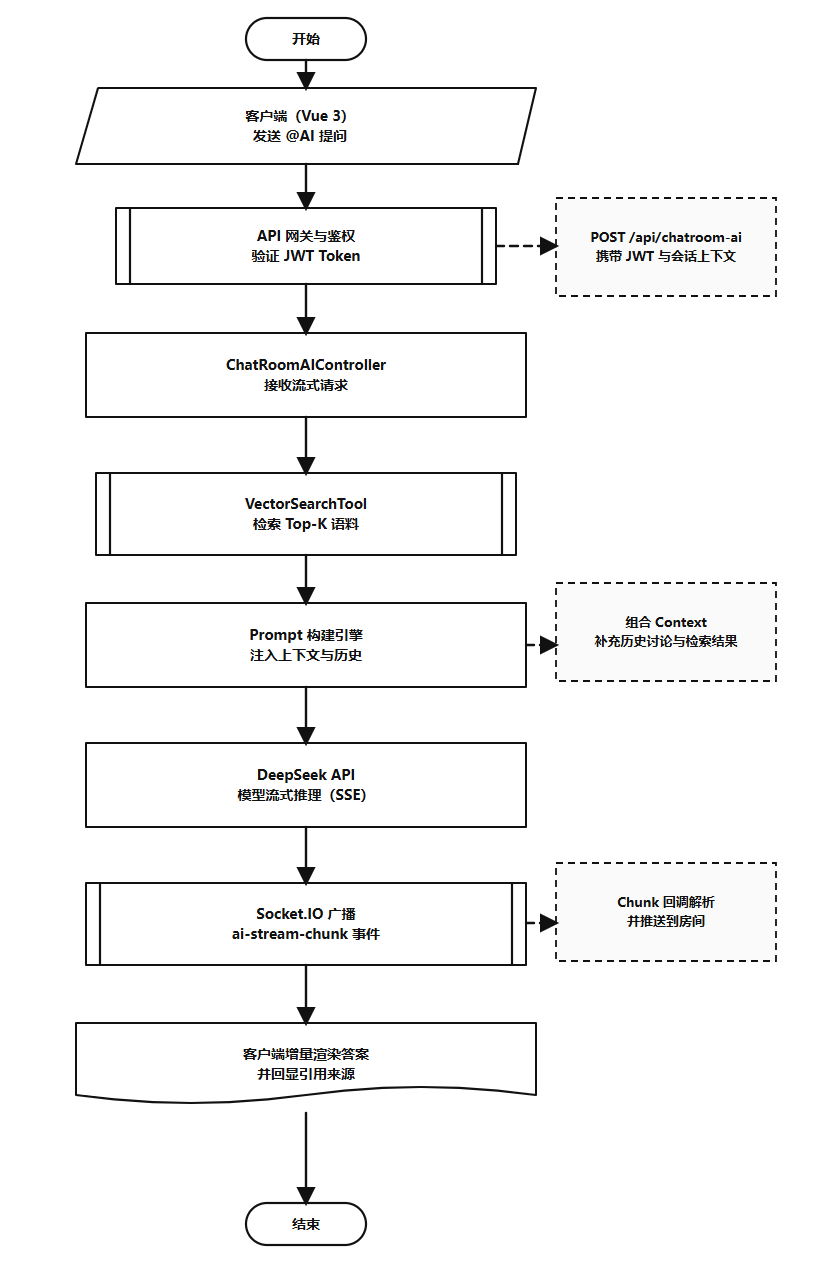
\includegraphics[width=0.94\textwidth,height=0.58\textheight,keepaspectratio]{img/图5_1.png}
\caption{RAG智能流式问答核心处理流}
\label{fig:5-20}
\end{figure}

如图~\ref{fig:5-20}所示，系统先通过向量检索工具在 MongoDB 历史集合中检索 Top-5 相关聊天记录，并将结果整理进 Prompt，再向模型发起流式请求。

在拼装好检索上下文后，后端会发起流式模型请求，并把增量内容同时写回 SSE 响应和ai流式广播事件。这样一来，提问者和同房间成员都能实时看到回答逐段生成。

该接口把 HTTP 的 SSE 响应和 WebSocket 房间广播结合在一起。提问者通过长连接逐步接收生成内容，同一房间内的其他成员则通过监听ai流式事件获取增量结果。对于响应耗时较长的大语言模型请求，这种分块返回机制能够缩短首字节等待时间（TTFB），也更适合多人协作场景\cite{deepseekrag2026}。

聊天室 AI 流式回复与结果落库的相关实现见附录D。

\subsubsection{WebSocket模块}

本系统通过 WebSocket 承载私聊通知、房间广播、在线状态同步以及协作类实时事件。实现上，私聊事件和房间级事件分开组织，语音交流和代码协作也单独拆分，从而避免所有实时逻辑堆叠在同一处\cite{socketiodocs2026,imsecurity2024}。

WebSocket 层分别维护“用户到 socket 集合”和“房间到在线用户集合”的映射关系，在广播消息前先完成连接归属和用户去重，再回推在线人数与消息增量。

WebSocket 层没有直接使用 \texttt{socket.id} 作为用户标识，而是建立了两层映射关系。私聊部分的用户表维护一个用户对应一组 socket 连接，从而支持同一账号在多个窗口同时登录；群聊部分的 \texttt{roomUsers} 记录“某个房间内在线的 userId 集合”，因此在线人数统计会按用户去重，避免同一用户的多窗口连接被重复计算。

此外，本系统没有将所有实时事件集中在同一个入口处理。私聊消息、群消息、语音连麦和代码协作分别独立实现，这样既便于后续按模块维护，也有助于在出现问题时快速定位具体事件链路。

房间在线状态维护与群消息广播的相关实现见附录E。

\subsubsection{数据模型与辅助模块}

后端在核心聊天主链路之外，还提供了上传、收藏、问题追踪、代码片段保存、消息索引和链接预览等辅助能力。这些模块共同支撑了技术交流场景下的信息保存、检索和回看需求。

群消息模型除了发送者、内容和时间等基础字段外，还扩展了引用回复、问题标记、表情反应和附件信息等结构，为收藏、历史检索和 AI 分析提供了统一的数据基础。

这一部分不仅补充了前端可见的功能入口，也补充了对应的数据结构。例如，引用回复、问题标记和表情反应都直接定义在消息模型中；收藏模块会保存消息快照，因此即使原消息被删除，收藏内容仍可回读；上传模块先保存文件，再将文件地址写回消息记录，使图片、语音和文件能够在历史消息中继续访问。此外，系统还通过消息向量化索引和RAG服务对文本消息进行向量化索引，为后续 AI 检索提供支持\cite{mongodbdocs2026,llmplatform2024}。

收藏数据写入与来源回读的相关实现见附录F。

\subsubsection{聊天室洞察与智能话题聚类分析}

对于一个活跃的技术交流平台，仅靠被动等待用户输入还不够，系统还需要具备整理房间讨论情况的能力。为此，本系统设计了 \texttt{getRoomInsights} 接口，用来汇总房间消息的整体状态。

\begin{figure}[H]
\centering
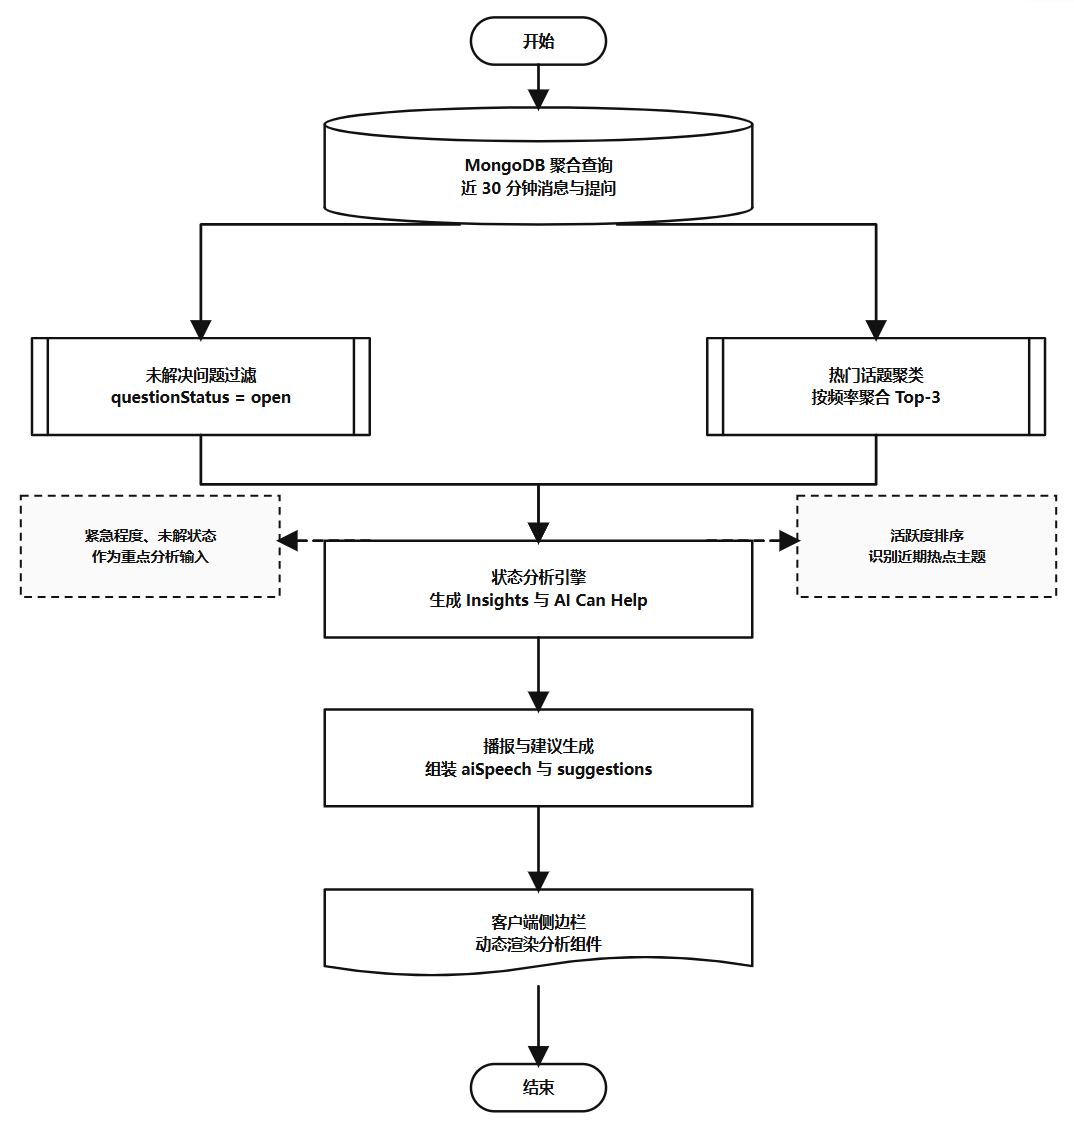
\includegraphics[width=0.94\textwidth,height=0.54\textheight,keepaspectratio]{img/图5_2.png}
\caption{聊天室实时洞察与状态分析流}
\label{fig:5-21}
\end{figure}

如图~\ref{fig:5-21}所示，该功能主要依靠 MongoDB 文档数据库的聚合能力完成统计，并未额外引入复杂的机器学习流程。

洞察模块先筛出未解决问题，再基于最近消息构建话题映射，统计讨论热度与参与者范围，最后把聚合结果整理成结构化的 \texttt{insights} 报告供前端展示。

系统先按时间窗口整理最近 30 分钟的数据，再利用 Map/Set 结构完成遍历和去重，最后把结果整理成扁平化的 \texttt{insights} 评估报告，并生成 \texttt{aiSpeech} 回传给前端展示。这样一来，用户可以直接看到哪些问题还没有解决、哪些话题仍在持续讨论，而不必完全依赖手动翻看消息记录。


\subsection{接口设计}

结合后端主入口、路由分发和具体业务处理逻辑，本系统常用接口可以分成普通 REST 接口、AI 接口和 WebSocket 通信接口三类。这里不把所有接口都逐一展开，而是挑出最能代表系统实现特点的几组进行说明，并结合表中内容概括每一类接口承担的职责。

\thesisparenitem{1}{普通 REST 接口设计}{这一部分主要包含用户认证、用户资料读取、私聊历史查询以及聊天室消息写入等标准 HTTP 请求接口。它们的共同特点是一次请求、一次返回，重点解决身份校验、数据持久化和列表查询等基础业务问题，是前端大多数页面能够正常工作的前提。普通 REST 接口的代表性设计如表~\ref{tab:5-1}所示。}

\begin{table}[!tbp]
\centering
\caption{普通 REST 接口设计}
\label{tab:5-1}
\small
\renewcommand{\arraystretch}{1.15}
\setlength{\tabcolsep}{0.7ex}
\begin{tabular}{M{0.16\textwidth}M{0.22\textwidth}M{0.10\textwidth}p{0.23\textwidth}p{0.19\textwidth}}
\toprule
\textbf{接口名称} & \textbf{请求路径} & \textbf{请求方式} & \textbf{参数说明} & \textbf{返回示例} \\
\midrule
发送验证码 & \parbox[t]{0.20\textwidth}{\raggedright \texttt{/api/user/}\\\texttt{send-verification}} & POST & \texttt{email}、\texttt{type} & 返回提示信息 \\
邮箱密码登录 & \texttt{/api/user/login-email} & POST & \texttt{email}、\texttt{password} & 返回 \texttt{token} 与用户信息 \\
获取当前用户信息 & \texttt{/api/user/info} & GET & Bearer Token & 返回 \texttt{user} 对象 \\
获取私聊消息 & \parbox[t]{0.20\textwidth}{\raggedright \texttt{/api/chat/}\\\texttt{messages/:id}} & GET & 路径参数为对方用户 ID & 返回消息数组 \\
发送群聊消息 & \parbox[t]{0.20\textwidth}{\raggedright \texttt{/room/:roomId/}\\\texttt{messages}} & POST & \texttt{content}、\texttt{messageType}、\texttt{quotedMessage} 等 & 返回消息对象 \\
\bottomrule
\end{tabular}
\end{table}

\noindent 表~\ref{tab:5-1}所列接口主要承担数据写入和稳定读取的任务。其中，登录、发送验证码和获取当前用户信息属于用户域接口，私聊消息读取和聊天室消息发送则属于会话域接口。这类接口并不追求长连接式的实时推送，而是强调参数明确、返回结构稳定和便于前后端分层调试。

\thesisparenitem{2}{AI 接口设计}{AI 接口主要服务于智能问答、文本解释和聊天总结等增强功能。与普通业务接口相比，它们通常需要拼接上下文、调用检索服务并进一步请求大语言模型，因此返回结果中不仅包含答案正文，还可能包含来源信息、置信度或结构化摘要内容。AI 接口的代表性设计如表~\ref{tab:5-2}所示。}

\begin{table}[!tbp]
\centering
\caption{AI 接口设计}
\label{tab:5-2}
\small
\renewcommand{\arraystretch}{1.15}
\setlength{\tabcolsep}{0.7ex}
\begin{tabular}{M{0.16\textwidth}M{0.22\textwidth}M{0.10\textwidth}p{0.23\textwidth}p{0.19\textwidth}}
\toprule
\textbf{接口名称} & \textbf{请求路径} & \textbf{请求方式} & \textbf{参数说明} & \textbf{返回示例} \\
\midrule
侧边栏智能问答 & \texttt{/api/agent/chat} & POST & \texttt{question}、\texttt{chatType}、\texttt{sessionId} 等 & 返回答案、来源和置信度 \\
会话总结 & \texttt{/api/agent/summarize} & POST & \texttt{chatType}、\texttt{targetId/roomId}、\texttt{timeRange} & 返回结构化总结 \\
划词解释 & \texttt{/api/agent/explain} & POST & \texttt{text}、\texttt{isFollowUp} & 返回解释文本 \\
聊天室流式问答 & \parbox[t]{0.20\textwidth}{\raggedright \texttt{/api/chatroom-ai/}\\\texttt{ask-stream}} & POST & \texttt{roomId}、\texttt{question}、\texttt{useRAG} & 以 SSE 分块返回结果 \\
\bottomrule
\end{tabular}
\end{table}

\noindent 表~\ref{tab:5-2}反映出，AI 接口并不是单一的一条问答接口，而是根据使用场景分成了侧边栏智能问答、会话总结、划词解释和聊天室流式问答四种类型。这样的拆分有助于把单人查询、多轮解释”和多人协作中的 AI 区分开来，也方便前端在不同页面里选择更合适的交互方式。

\thesisparenitem{3}{WebSocket 通信接口设计}{WebSocket 部分主要用于处理用户上线注册、私聊消息通知、加入聊天室、群消息广播以及 AI 流式输出同步等事件。它与前两类接口最大的不同，在于它强调服务端主动推送和多端实时同步，更适合承载聊天系统里的在线状态与增量消息场景。WebSocket 通信接口的代表性设计如表~\ref{tab:5-3}所示。}

\begin{table}[!tbp]
\centering
\caption{WebSocket 通信接口设计}
\label{tab:5-3}
\small
\renewcommand{\arraystretch}{1.15}
\setlength{\tabcolsep}{0.7ex}
\begin{tabular}{M{0.15\textwidth}M{0.20\textwidth}M{0.10\textwidth}p{0.24\textwidth}p{0.20\textwidth}}
\toprule
\textbf{接口名称} & \textbf{通信标识} & \textbf{触发方式} & \textbf{参数说明} & \textbf{返回示例} \\
\midrule
用户上线注册 & \texttt{login} & client emit & \texttt{userId} & 服务端登记在线状态并回推列表 \\
私聊消息通知 & \texttt{private-message} & 双向 & \texttt{from}、\texttt{to}、\texttt{content} 等 & 实时推送私聊消息 \\
加入聊天室 & \texttt{join-group} & client emit & \texttt{roomId}、\texttt{userId} & 触发在线人数和成员广播 \\
群消息广播 & \texttt{group-message} & 双向 & \texttt{roomId}、\texttt{content}、\texttt{fromName} 等 & 房间成员收到完整消息对象 \\
AI 增量输出 &ai流式& server emit & \texttt{roomId}、\texttt{content}、\texttt{isComplete} & 前端逐段渲染 AI 回答 \\
\bottomrule
\end{tabular}
\end{table}

\noindent 表~\ref{tab:5-3}反映出系统实时通信层的核心职责，即把“谁上线了”“谁加入了房间”“哪条消息需要立即同步给谁”这些高频事件从普通 HTTP 请求中拆出来单独处理。尤其是 \texttt{group-message} 与ai流式这类事件，直接决定了聊天室消息和 AI 回答能否在界面上即时呈现。

\FloatBarrier

\subsection{示例数据}

为了说明接口返回内容，下面给出两个更贴近实际格式的示例。字段名与系统实际返回结构保持一致，只对 token 和部分 ID 做了简化。

\thesisparenitem{1}{示例 1：邮箱密码登录接口返回}{返回体通常包含 \texttt{message}、\texttt{token} 和 \texttt{user} 三部分，其中 \texttt{user} 内含用户 ID、昵称、邮箱与头像地址，足以支撑前端完成登录后的首轮渲染。}

\thesisparenitem{2}{示例 2：智能问答接口返回}{返回体会以 \texttt{success} 标记请求结果，并在 \texttt{data} 中给出回答正文、来源片段、置信度、是否使用上下文以及检索条数等信息，用于前端展示答案与解释其生成依据。}

\subsection{通信机制说明}

\subsubsection{HTTP 通信流程}

普通业务请求大多遵循同一条链路：前端通过 Axios 发起请求，并在请求头中附带 token；服务端经过认证模块完成鉴权后，再进入具体业务处理；随后由数据模型读写 MongoDB，并将 \texttt{user}、消息记录等结果返回给前端。登录、获取当前用户信息、拉取历史消息、上传文件和创建聊天室等操作基本都按这一流程完成\cite{expressdocs2026,mongodbdocs2026}。

\subsubsection{WebSocket 实时通信流程}

实时通信与 HTTP 在系统中承担不同职责。HTTP 主要负责数据写入与读取，Socket.IO 则负责将状态变化和消息增量及时同步给在线成员。私聊发送时，前端通常先通过 REST 接口写库，再发送 \texttt{private-message} 通知对方刷新；群聊发送时，客户端完成消息提交后，由服务端主动广播 \texttt{group-message}，房间成员据此刷新列表和未读状态。客户端建立连接后，还会先完成 \texttt{login} 与 \texttt{join-group} 等注册动作。这种拆分能够将消息持久化与实时同步分别验证\cite{socketiodocs2026}。

\subsubsection{AI 请求调用流程}

AI 请求比普通接口多了一层上下文和检索处理。侧边栏 AI 助手会先进入 AI 处理链路，再按顺序完成最近消息提取、RAG 检索和答案生成，最后返回回答正文、来源和置信度。聊天室里的 \texttt{@AI} 更偏向实时协作，系统会先补足上下文，再请求流式模型接口，并把分块结果同时写回 HTTP 响应和房间广播事件\cite{qaoverview2025,ragsurveycn2025,deepseekrag2026}。

\subsection{展示内容}

为了保证接口文档与系统实现保持一致，本系统在联调阶段使用 Swagger 页面逐项核对主要 REST 接口，包括用户认证、聊天室消息、收藏和 AI 相关请求。接口文档界面如图~\ref{fig:5-1}所示，它能够直接展示请求方法、路径、参数结构和调试入口，对后续接口联调和答辩演示都比较直观。

\begin{figure}[H]
\centering
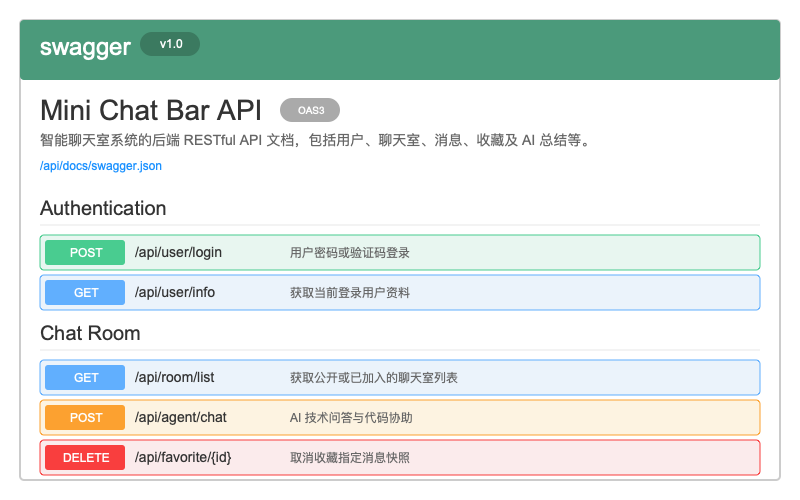
\includegraphics[width=0.88\textwidth,height=0.36\textheight,keepaspectratio]{img/图5_3.png}
\caption{Swagger 接口文档}
\label{fig:5-1}
\end{figure}

后端运行日志能够反映接口进入、Socket 连接和 AI 请求发起等关键状态。将这一部分保留在论文中，有助于更直观地说明系统运行过程中的联调与验证依据。

例如登录接口返回、聊天室消息拉取、Socket 建连和 AI 接口调用，都会在控制台留下时间戳、访问路径和耗时信息，便于联调阶段快速定位问题。

\FloatBarrier

\section{Web前端实现}

前端实现主要集中在 \texttt{ccb/src} 目录下。该部分没有完全按照技术层拆分，而是更接近功能模块划分：登录页、聊天主界面、AI 助手、消息管理和设置页分别对应独立组件或页面。这种组织方式便于围绕具体功能进行维护和定位\cite{vueguide2026,piniadocs2026,electrondocs2026}。

其中，聊天主界面的路由切换逻辑和收藏页的筛选、详情回看逻辑共同构成了前端核心交互。

\subsection{登录/注册页面}

\thesisparenitem{1}{界面功能说明}{登录和注册页面采用翻转卡片形式，正面为登录，背面为注册。登录又分为邮箱密码和邮箱验证码两种方式，卡片底部保留了 Google 和 GitHub 的第三方登录按钮。页面同时提供欢迎信息、输入反馈和登录方式切换，如图~\ref{fig:5-2}和图~\ref{fig:5-3}所示。}

\thesisparenitem{2}{关键交互逻辑}{用户输入邮箱和密码后，前端会先进行格式校验。对于邮箱格式错误、密码为空，或注册时两次密码不一致等情况，页面会在前端阶段直接拦截无效请求。验证码登录额外包含冷却时间控制，60 秒内不能重复获取验证码。登录成功后，页面不仅保存 token，还会继续调用 \texttt{waitForSocketConnection()}，在 Socket 成功连接后发出 \texttt{login} 和 \texttt{user-online} 事件，以完成在线状态初始化。}

\thesisparenitem{3}{与后端的接口交互说明}{邮箱密码登录调用 \texttt{/api/user/\allowbreak login-email}，验证码登录调用 \texttt{/api/user/\allowbreak login-code}，发送验证码调用 \texttt{/api/user/\allowbreak send-verification}，注册调用 \texttt{/api/user/\allowbreak register-email}，第三方登录则直接跳转到 \texttt{/auth/\allowbreak google} 和 \texttt{/auth/\allowbreak github}。}

\thesisparenitem{4}{操作流程}{用户先进入登录页，选择密码登录、验证码登录或第三方登录；若采用本地登录，则输入表单并提交；后端验证通过后返回 token 和用户资料；前端随后保存登录信息、初始化在线状态和 Socket 连接，最后跳转到聊天主界面。}

\begin{figure}[H]
\centering
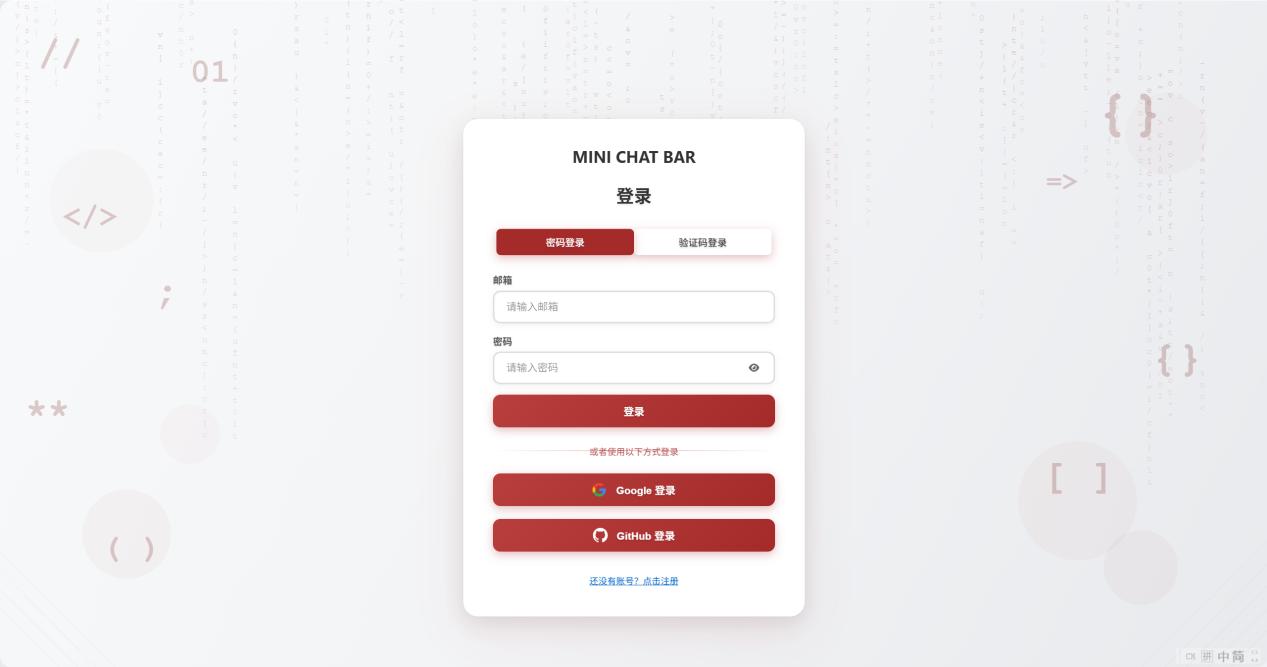
\includegraphics[width=0.88\textwidth,height=0.36\textheight,keepaspectratio]{img/图5_4.png}
\caption{登录页面展示}
\label{fig:5-2}
\end{figure}

\begin{figure}[H]
\centering
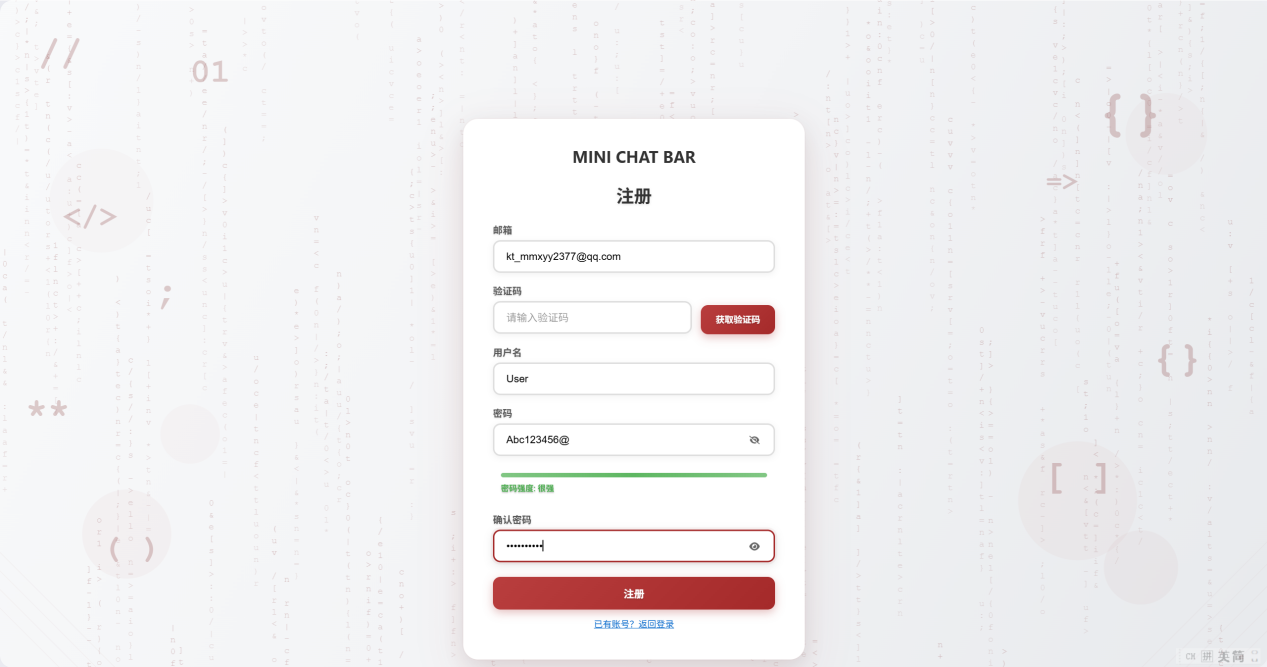
\includegraphics[width=0.88\textwidth,height=0.36\textheight,keepaspectratio]{img/图5_5.png}
\caption{注册页面与表单交互展示}
\label{fig:5-3}
\end{figure}

\FloatBarrier

\subsection{聊天主界面}

\thesisparenitem{1}{界面功能说明}{桌面端采用三栏布局，左侧为导航入口，中间为会话或联系人列表，右侧为详情区；移动端则切换为底部导航形式。该页面主要承担路由组织和区域切换职责，根据当前路由和用户操作决定中间栏与右侧区域的显示内容。主界面总览如图~\ref{fig:5-5}所示，通讯录和聊天室入口分别如图~\ref{fig:5-6}、图~\ref{fig:5-7}所示。}

这一部分对应的前端路由切换与界面组织逻辑见附录G。

\thesisparenitem{2}{关键交互逻辑}{页面初始化时，前端会先检查登录状态，再根据当前路由决定默认展示聊天列表、联系人列表或聊天室列表。用户点击左侧导航栏或底部导航时，页面通过路由切换对应内容区域，而不是仅在界面层隐藏某一块 DOM。用户进入具体联系人或房间后，\texttt{showdetail()} 展示详情函数会将当前目标 ID 写入 \texttt{useChatStore}，并同步传递昵称、头像和聊天类型等参数，为后续消息加载与状态同步提供上下文。}

\thesisparenitem{3}{与后端的接口交互说明}{主界面本身不直接发送消息，但会触发好友列表、群列表、聊天室列表以及用户信息等接口的请求。常见调用包括 \texttt{/api/user/info}、\texttt{/api/user/friends}、\texttt{/room/list} 和 \texttt{/room/chatrooms}。}

\thesisparenitem{4}{操作流程}{用户登录进入主界面后，前端先加载基础资料和列表数据；再根据当前需求切到聊天、联系人或聊天室；选择具体会话后，前端写入当前会话上下文并跳转详情页；详情页继续拉取消息记录并建立需要的 Socket 监听。}

\begin{figure}[H]
\centering
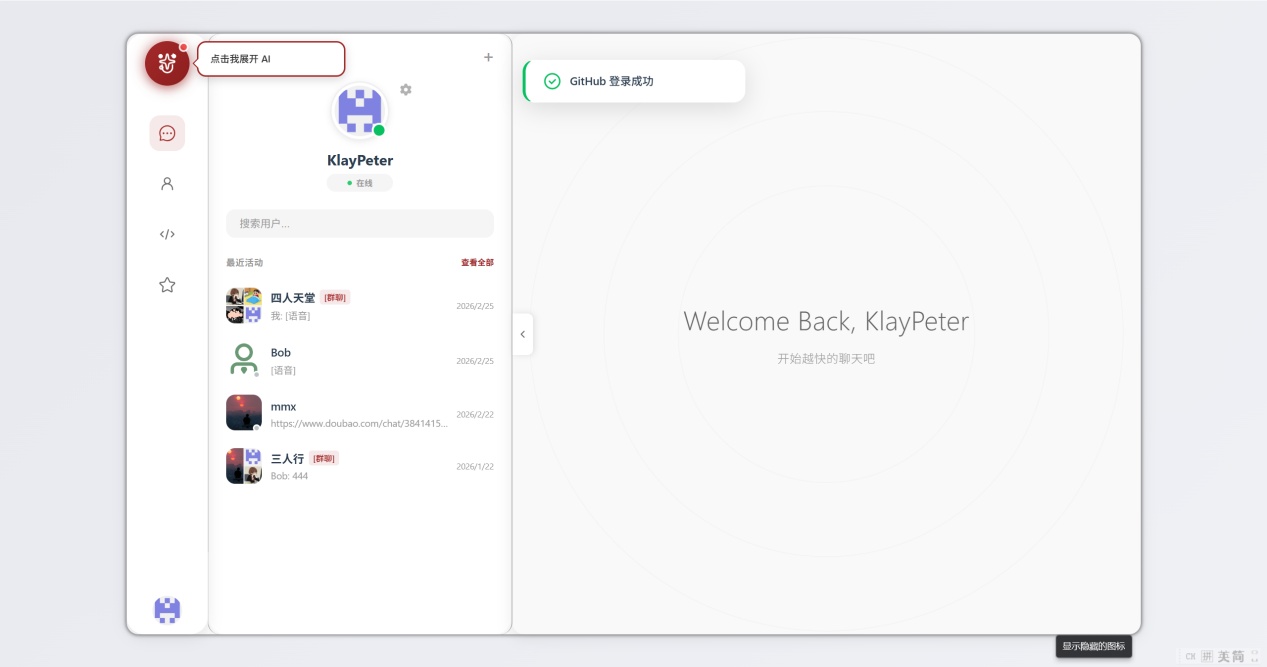
\includegraphics[width=0.88\textwidth,height=0.36\textheight,keepaspectratio]{img/图5_7.png}
\caption{聊天主界面总览}
\label{fig:5-5}
\end{figure}

\begin{figure}[H]
\centering
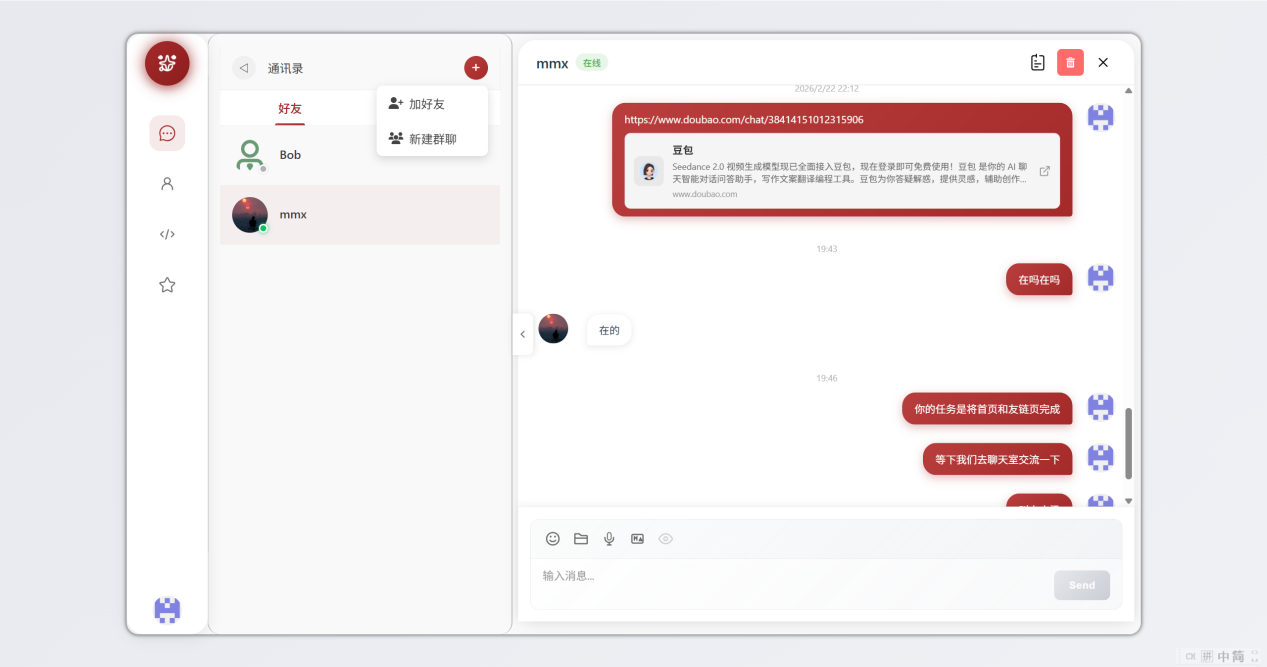
\includegraphics[width=0.88\textwidth,height=0.36\textheight,keepaspectratio]{img/图5_8.png}
\caption{通讯录列表界面展示}
\label{fig:5-6}
\end{figure}

\begin{figure}[H]
\centering
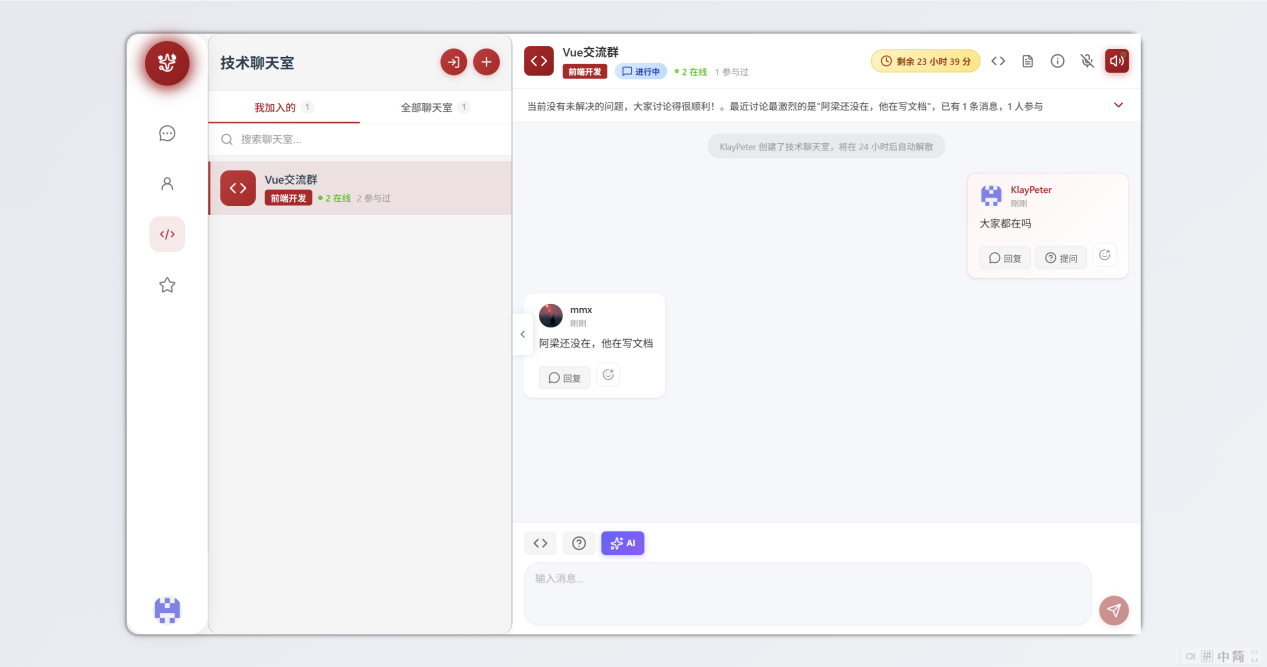
\includegraphics[width=0.88\textwidth,height=0.36\textheight,keepaspectratio]{img/图5_9.png}
\caption{聊天室列表界面展示}
\label{fig:5-7}
\end{figure}

\FloatBarrier

\subsection{AI对话界面}

\thesisparenitem{1}{界面功能说明}{AI 对话相关的界面有两种典型形态。第一种是侧边栏 AI 助手，适合做单独问答、补充解释和上下文延续；第二种是聊天室里的 \texttt{@AI} 交互，它把 AI 回答直接放回房间消息流，更适合多人讨论时一起参考。侧边栏 AI 助手界面如图~\ref{fig:5-9}所示，聊天室中的 AI 回答效果如图~\ref{fig:5-10}所示。}

\thesisparenitem{2}{关键交互逻辑}{侧边栏模式下，用户输入的问题会先追加到本地消息数组，再调用 \texttt{/api/agent/chat} 请求答案，请求成功后再把 AI 回复和来源信息追加到界面。聊天室模式则更强调实时感。用户在输入框里直接输入 \texttt{@AI} 开头的问题，前端会先把原问题发进房间，再触发 \texttt{/api/chatroom-ai/ask-stream}，然后一边接收流式内容，一边刷新当前房间的消息列表。因为后端会把 AI 输出同步广播到房间，所以这个回答不是只对提问者可见，而是房间成员都能看到。}

\thesisparenitem{3}{与后端的接口交互说明}{侧边栏模式主要依赖智能问答和解释接口，聊天室模式则围绕流式问答、智能提示和主动答题几类接口展开。}

\thesisparenitem{4}{操作流程}{AI 模块的操作流程可以概括为：用户打开 AI 面板或在聊天室中输入 \texttt{@AI}；前端提交问题并附带当前上下文；后端结合最近消息和历史检索结果生成回答；回答返回后，前端再按普通消息或流式消息渲染出来。}

\begin{figure}[H]
\centering
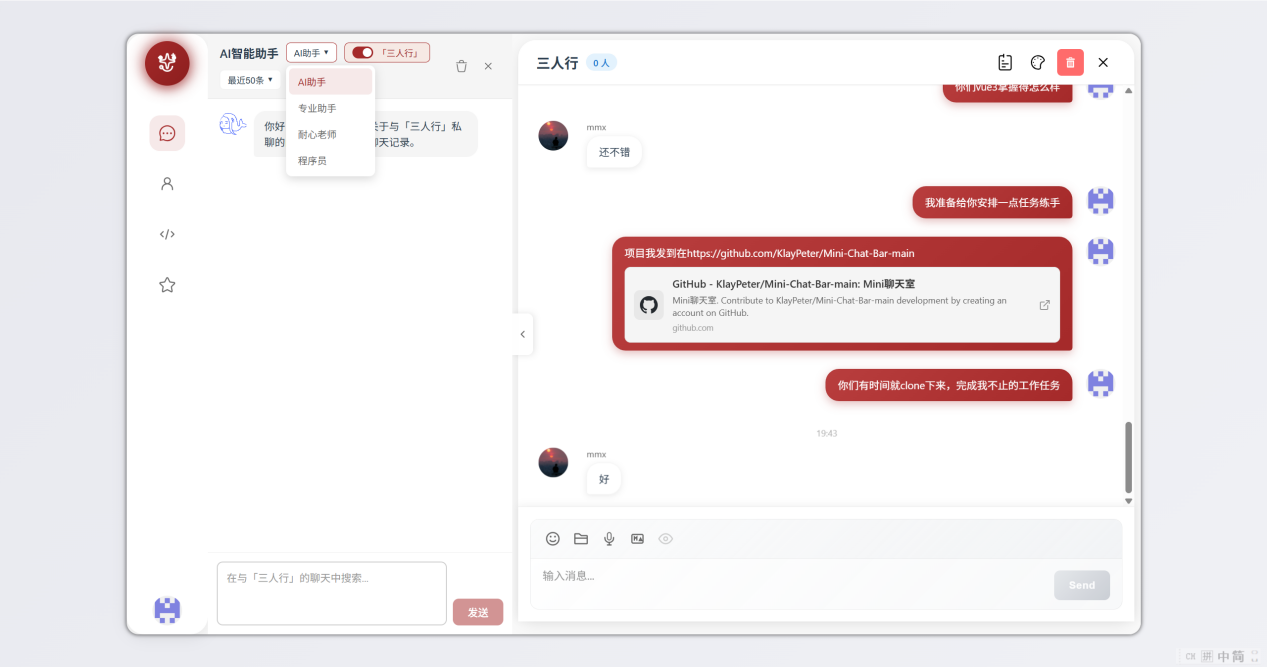
\includegraphics[width=0.88\textwidth,height=0.36\textheight,keepaspectratio]{img/图5_11.png}
\caption{侧边栏 AI 助手界面}
\label{fig:5-9}
\end{figure}

\begin{figure}[H]
\centering
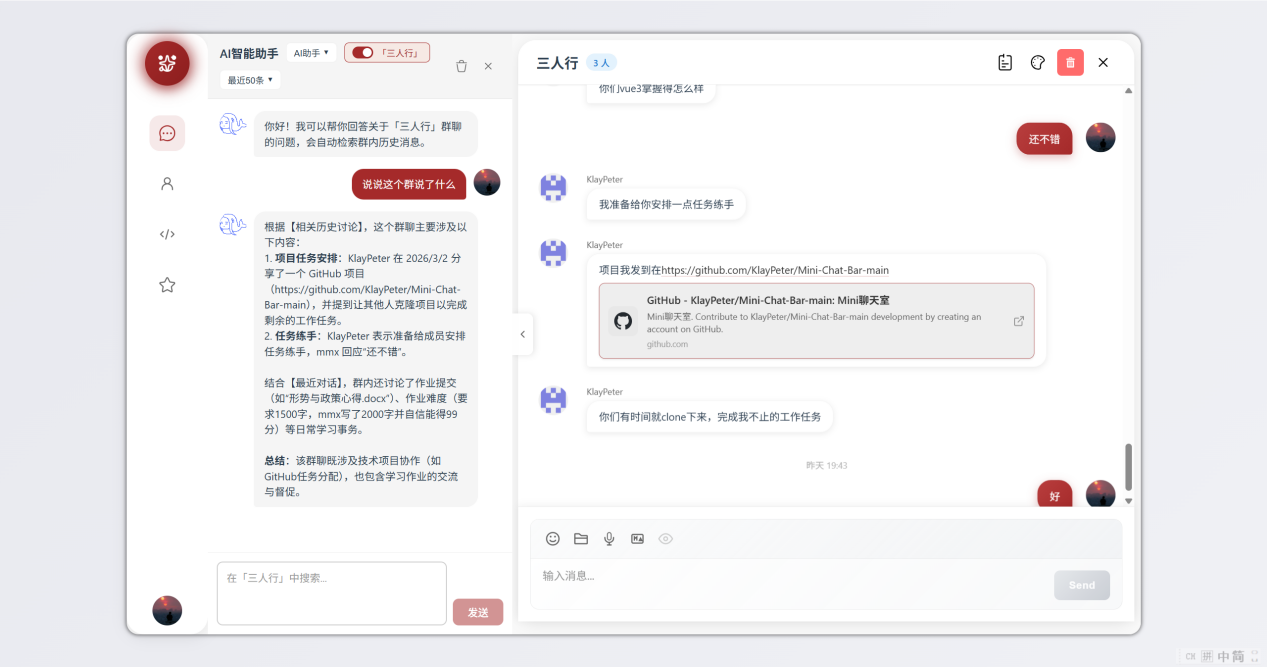
\includegraphics[width=0.88\textwidth,height=0.36\textheight,keepaspectratio]{img/图5_12.png}
\caption{AI 根据历史记录检索后的回答展示}
\label{fig:5-10}
\end{figure}

\FloatBarrier

\subsection{消息列表与会话管理}

\thesisparenitem{1}{界面功能说明}{该部分不仅展示消息列表，还负责最近会话排序、未读数显示、历史消息搜索、收藏整理以及消息转发、撤回等行为。最近会话列表和消息页结合后的效果如图~\ref{fig:5-12}所示，历史消息搜索和收藏页分别如图~\ref{fig:5-13}、图~\ref{fig:5-14}所示。}

\thesisparenitem{2}{关键交互逻辑}{会话列表加载时，前端会先读取好友列表，再查询每个联系人和群聊的最后一条消息及未读数，并按时间重新排序。当前会话打开后，页面继续加载完整历史记录，并按消息类型进行分类渲染。用户点击搜索图标时，前端会在当前消息数组中进行关键词匹配并高亮结果；点击收藏时，则将消息 ID、消息类型和会话 ID 一并发送给后端，以便后续在收藏页单独回看。}

\thesisparenitem{3}{与后端的接口交互说明}{该部分会频繁调用 \texttt{/api/chat/\allowbreak last\_message/\allowbreak :id}、\texttt{/api/chat/\allowbreak unread}、\texttt{/api/chat/\allowbreak messages/\allowbreak :id} 等消息接口，以及 \texttt{/room/\allowbreak :roomId/\allowbreak messages}、\texttt{/api/\allowbreak favorites} 和 \texttt{/api/\allowbreak favorites/\allowbreak :messageId} 等房间与收藏接口。}

\thesisparenitem{4}{操作流程}{消息列表与会话管理的基本流程是：先加载会话摘要信息，再根据用户选择打开具体会话；进入会话后加载完整历史消息；如果用户执行搜索、收藏或删除等操作，再分别调用对应接口更新状态，并同步刷新列表（相关实现见附录H）。}

\begin{figure}[H]
\centering
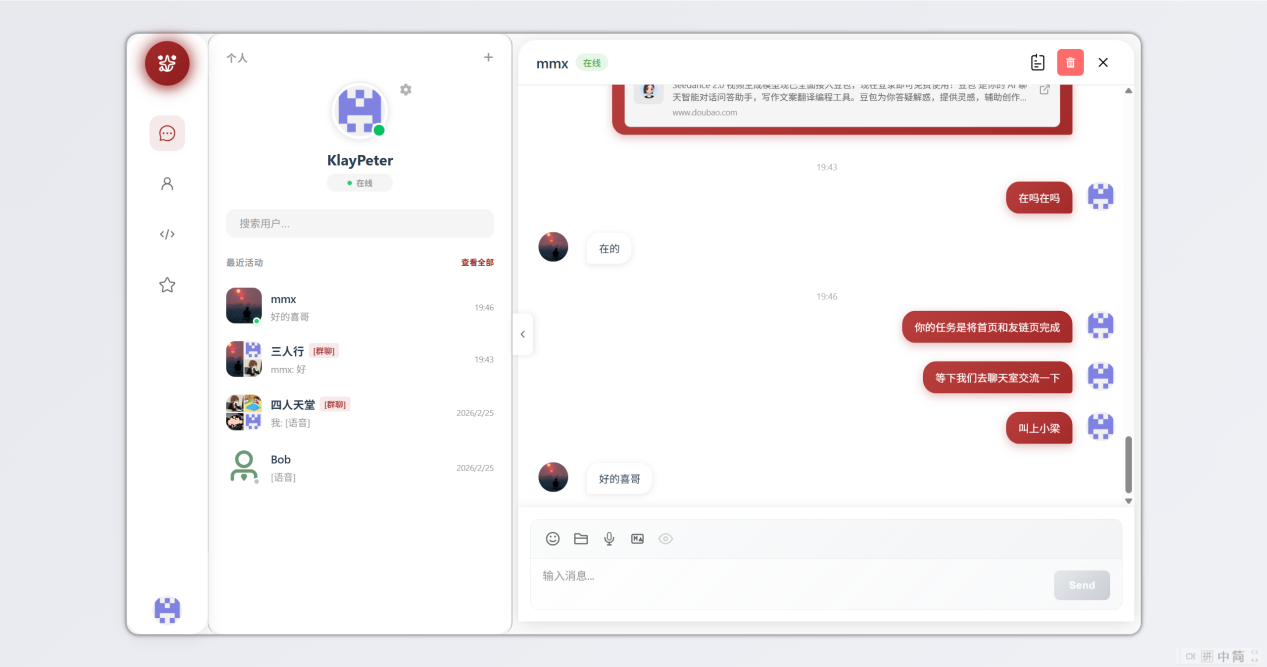
\includegraphics[width=0.88\textwidth,height=0.36\textheight,keepaspectratio]{img/图5_14.png}
\caption{会话列表与私聊界面展示}
\label{fig:5-12}
\end{figure}

\begin{figure}[H]
\centering
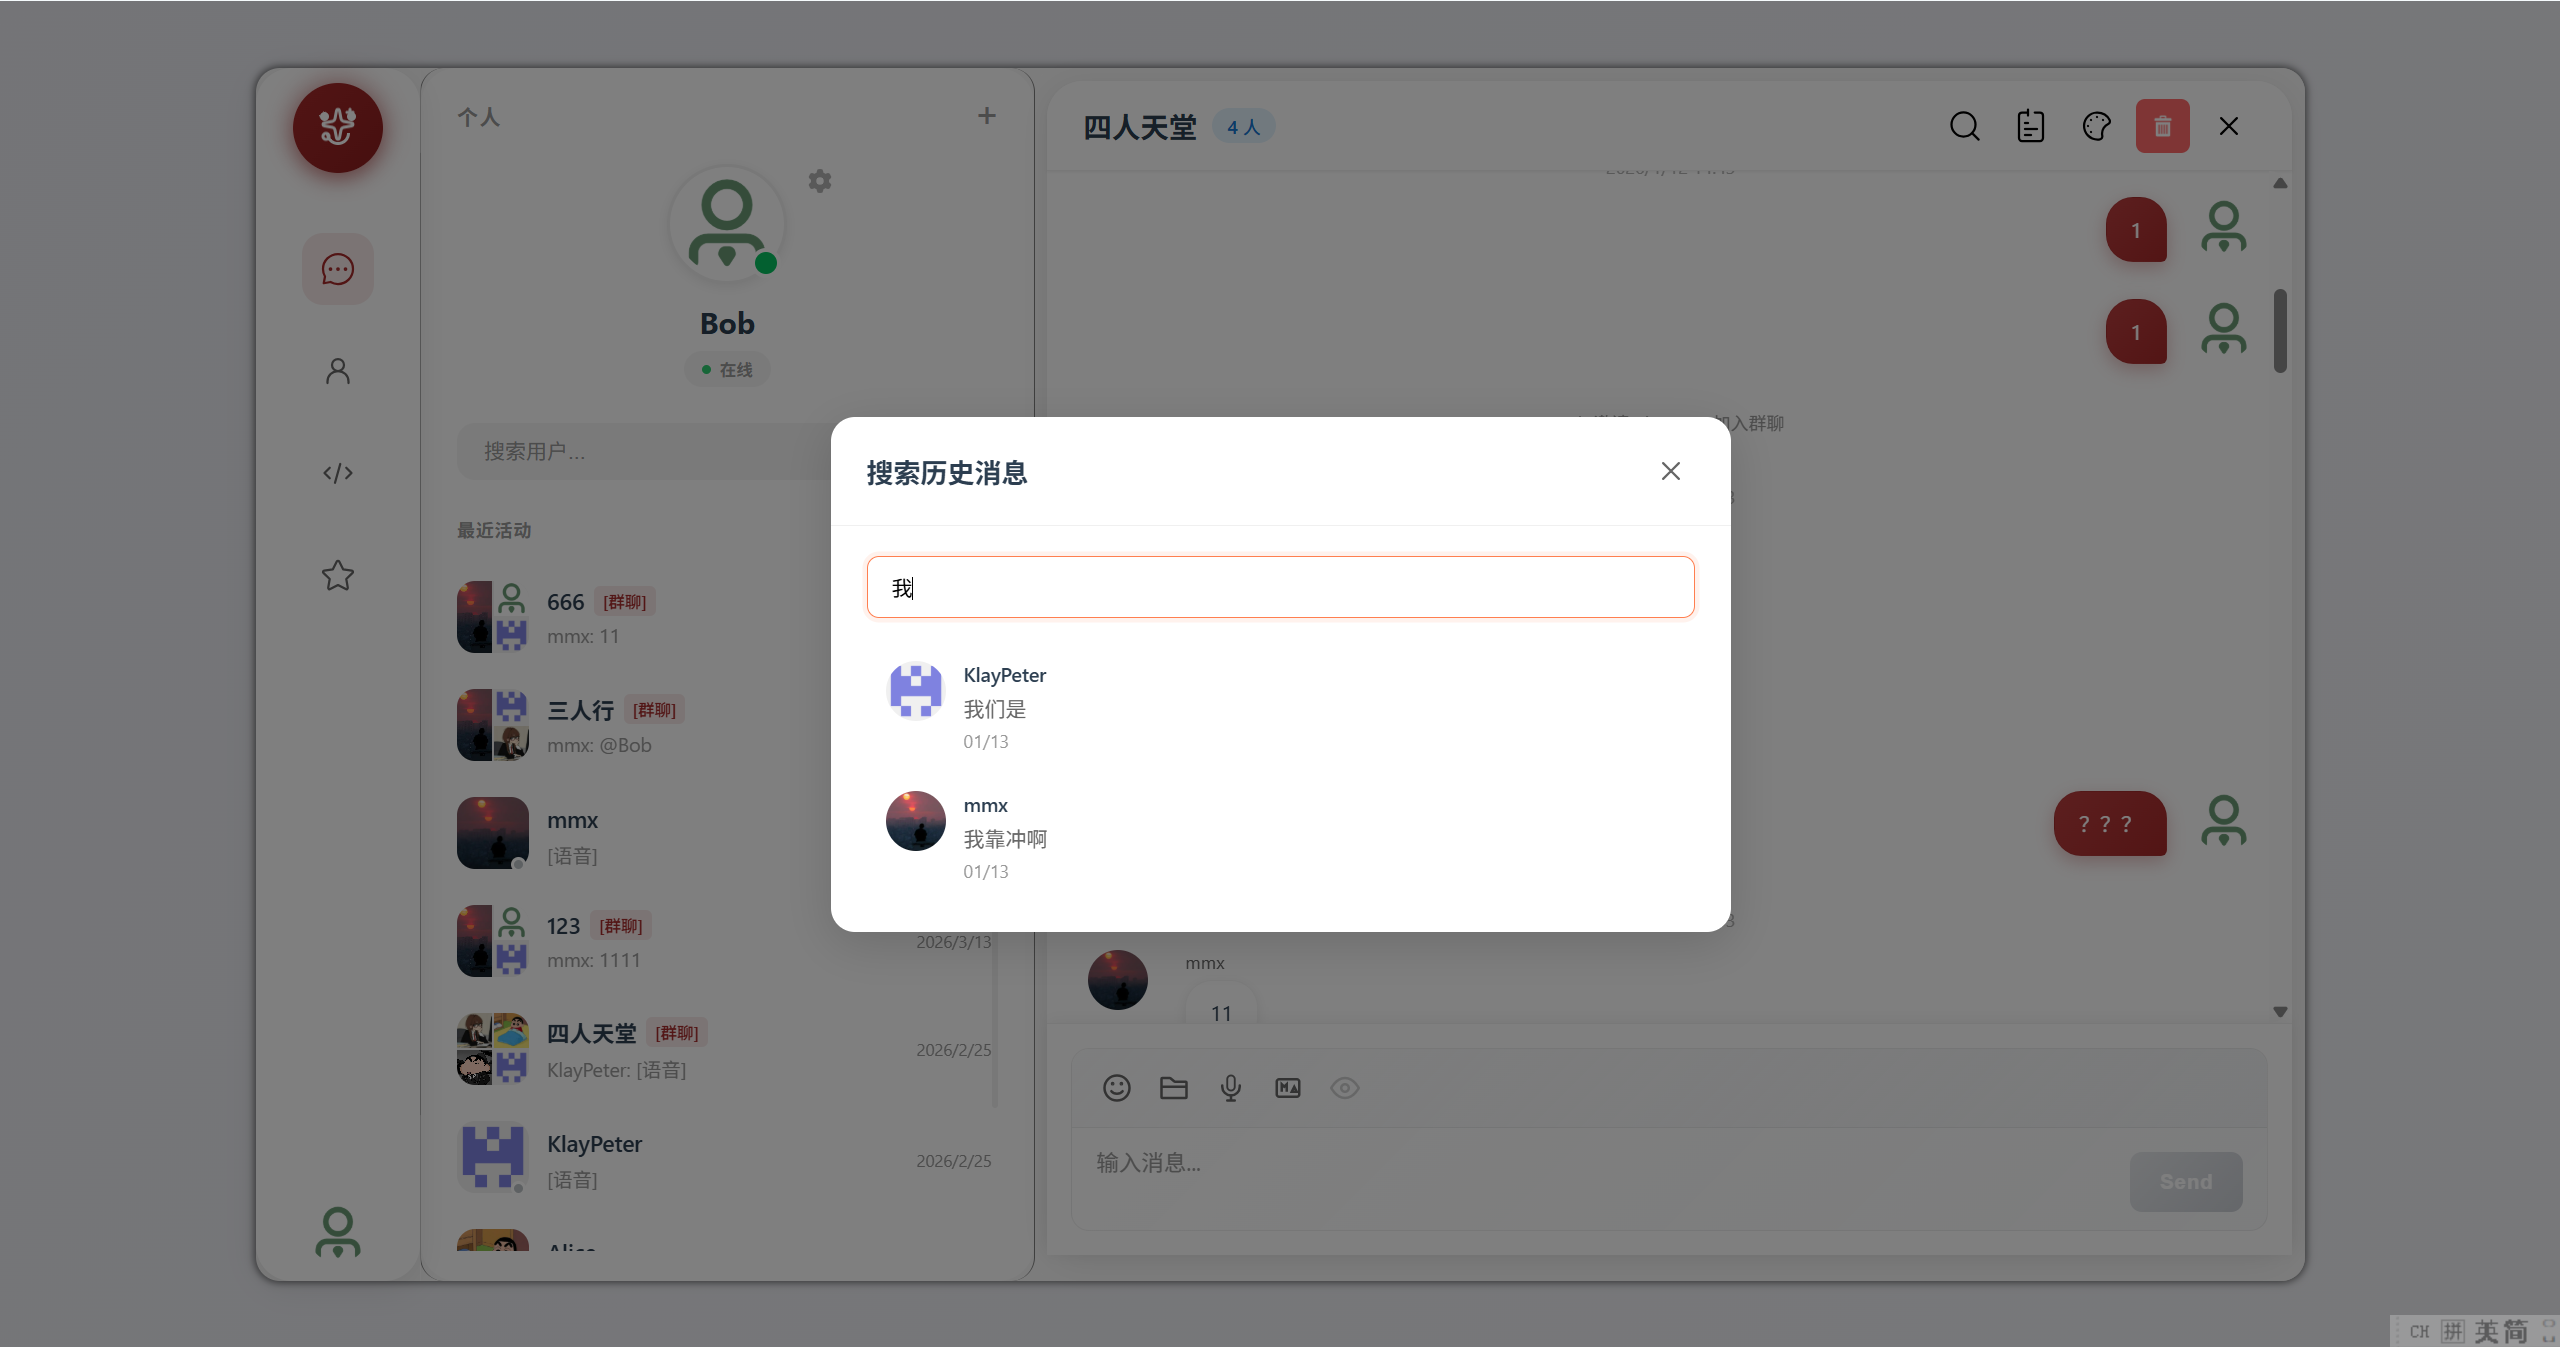
\includegraphics[width=0.88\textwidth,height=0.36\textheight,keepaspectratio]{img/图5_15.png}
\caption{历史消息搜索界面展示}
\label{fig:5-13}
\end{figure}

\begin{figure}[H]
\centering
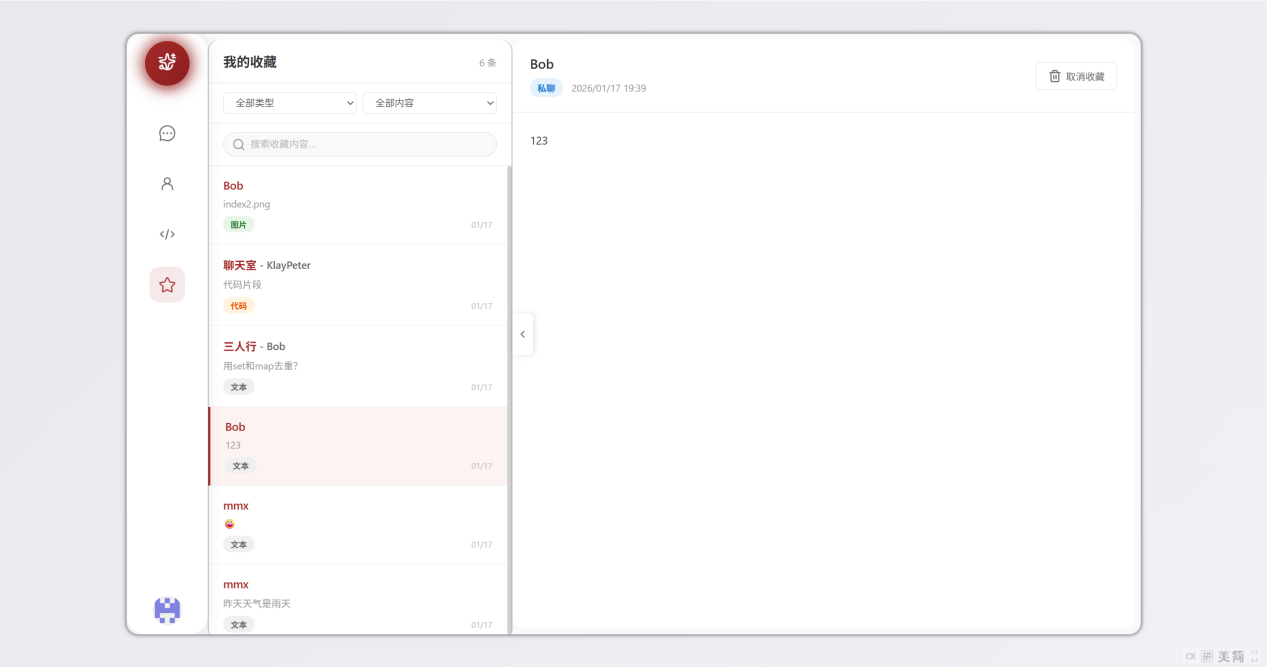
\includegraphics[width=0.88\textwidth,height=0.36\textheight,keepaspectratio]{img/图5_16.png}
\caption{收藏页面展示}
\label{fig:5-14}
\end{figure}

\FloatBarrier

\subsection{设置与个人中心}

\thesisparenitem{1}{界面功能说明}{设置与个人中心包含头像上传、预设头像切换、用户名修改、主题切换和退出登录等功能。该模块虽然不像聊天页那样集中承载消息交互，但与主界面的资料展示保持联动。用户更新头像后，最近会话列表、当前聊天页和其他在线用户看到的资料都需要同步刷新。设置与个人中心界面的实际效果如图~\ref{fig:5-16}所示。}

\thesisparenitem{2}{关键交互逻辑}{用户上传头像时，前端先把图片发到 \texttt{/api/upload}，拿到文件地址后再调用 \texttt{/api/user/avatar} 更新资料；修改用户名时，则直接调用 \texttt{/api/user/username}。更新成功后，前端会发出 \texttt{avatar-updated} 事件，通知其他在线用户同步刷新头像。主题切换则通过 \texttt{useThemeStore} 完成，并把主题键值写入 \texttt{localStorage}，这样刷新页面后仍然保留用户上一次的选择。}

\thesisparenitem{3}{与后端的接口交互说明}{头像上传依赖 \texttt{/api/upload}，资料更新依赖 \texttt{/api/user/\allowbreak avatar} 和 \texttt{/api/user/\allowbreak username}，界面刷新时则重新读取 \texttt{/api/user/\allowbreak info}。}

\thesisparenitem{4}{操作流程}{设置模块的基本流程为：用户打开设置弹窗，修改头像、用户名或主题；前端调用对应接口并保存结果；保存成功后，同步刷新本地资料和相关组件；如果修改内容会影响其他在线用户的显示结果，还会继续通过 Socket 广播更新。}

\begin{figure}[H]
\centering
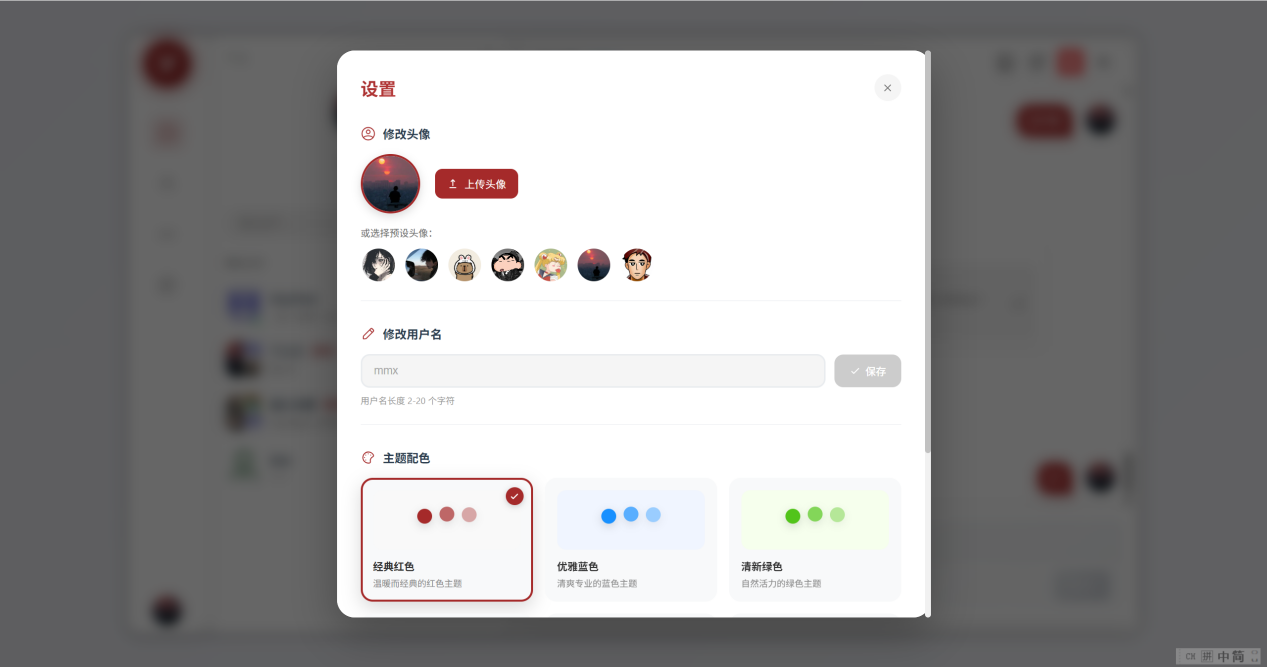
\includegraphics[width=0.88\textwidth,height=0.36\textheight,keepaspectratio]{img/图5_18.png}
\caption{设置与个人中心界面展示}
\label{fig:5-16}
\end{figure}

\FloatBarrier

\subsection{Web端消息流转与状态管理}

从界面表现看，Web 端的核心功能集中在登录、消息收发和会话切换，而这些功能能稳定运行，依赖于底层的消息流转和状态管理。私聊发送时，系统会先调用 \texttt{/api/chat/messages/:id} 将消息写入数据库，再通过 \texttt{private-message} 事件提醒另一端刷新；群聊发送时，前端调用 \texttt{/room/:roomId/messages}，后端控制器保存成功后会主动广播 \texttt{group-message}，因此前端不需要重复发送同名消息。收到消息后，界面再根据 \texttt{messageType} 区分文本、图片、文件、语音和代码等不同渲染分支，从而完成统一消息列表中的分类展示。

WebSocket 的使用也做了分层处理。普通聊天页主要依赖socket提供的全局连接，这一层包含自动重连、断线提示和心跳包；聊天室详情页则额外维护房间级事件，包括 \texttt{join-group}、\texttt{online-count}、\texttt{ai-stream-chunk}、\texttt{join-voice-room} 等。这样一来，普通会话页和聊天室页就能分别承载不同复杂度的实时交互。

状态管理方面，系统虽然使用了 Pinia，但并没有把所有状态都集中到全局 store。全局配置文件只保留 \texttt{currentChatUser} 和按用户区分的消息列表；会话列表、未读数、当前房间详情、搜索结果和收藏状态等内容，仍由各组件内部的 \texttt{ref} 与自定义事件配合维护。比如群聊消息发送后，前端会发出 \texttt{group-message-sent} 事件通知列表刷新；聊天室打开后，再通过 \texttt{group-chat-opened} 事件清除未读数。这样的组织方式和当前项目规模基本匹配。

\FloatBarrier

\section{桌面端实现}

桌面端在界面层仍复用了同一套前端页面，但额外增加了 Electron 封装。因此，它与 Web 端的主要差异不在聊天主流程本身，而在窗口管理、系统托盘、本地通知和 IPC 通信等桌面环境能力。

\subsection{系统托盘功能}

桌面端由 Electron 主进程统一管理窗口和托盘行为。程序启动后会先创建主窗口，再创建托盘图标。在 Windows 下，用户关闭主窗口时，程序不会直接退出，而是隐藏到系统托盘继续运行。托盘左键用于显示或隐藏主窗口，右键菜单提供“打开应用”和“退出应用”两个入口，这样桌面端就能在后台继续接收消息。

托盘点击事件会在“显示主窗口”和“隐藏到后台”之间切换，保证程序关闭窗口后仍可保持驻留状态和未读提醒能力。

桌面端在收到新消息后的未读提醒和任务栏反馈效果如图~\ref{fig:5-18}所示。这个设计是在复用网页界面的基础上，补充桌面环境下的消息提醒机制。

\begin{figure}[H]
\centering

\includegraphics[width=0.88\textwidth,height=0.36\textheight,keepaspectratio]{img/图5_20.png}
\caption{桌面端未读提醒展示}
\label{fig:5-18}
\end{figure}

\FloatBarrier

\subsection{本地通知}

本地通知由消息提醒管理模块、预加载脚本和 Electron 主进程三部分配合完成。渲染进程收到新消息后，会通过 \texttt{window.electronAPI.notifyNewMessage()} 把未读数发给主进程；主进程根据平台再去设置任务栏闪烁、Overlay 图标、托盘提示和最近消息预览。用户如果从托盘预览里点击某个会话，主进程还会继续把 \texttt{open-chat} 事件发回渲染进程，前端再切到对应私聊或群聊。

渲染进程把未读数和最近消息通过 \texttt{electronAPI} 发送给主进程后，主进程再统一负责闪烁提醒、角标更新和托盘预览，从而把桌面通知逻辑和业务页面分开处理（相关实现见附录I）。

系统托盘的图标、菜单入口与后台驻留形态如图~\ref{fig:5-19}所示。托盘机制使桌面端在关闭主窗口后仍能继续接收消息，并保留快速唤起入口。

\begin{figure}[H]
\centering
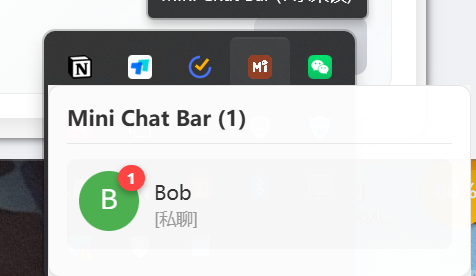
\includegraphics[width=0.88\textwidth,height=0.36\textheight,keepaspectratio]{img/图5_21.png}
\caption{系统托盘展示}
\label{fig:5-19}
\end{figure}

\FloatBarrier

\subsection{与后端和WebSocket通信}

桌面端和后端通信的基础方式并没有变化，仍然由 Axios 调用 REST 接口，并由 Socket.IO 负责实时同步。区别在于，桌面端比 Web 端多了一层由通信转接层暴露的 \texttt{electronAPI}，使渲染进程在不直接接触 Node API 的前提下，也能将“新消息提醒”“清空角标”“打开对应会话”等动作交给主进程处理。

从这一点看，桌面端并不是另一套独立业务系统，而是在 Web 端原有聊天逻辑之外补充桌面环境能力。这样可以保持核心业务代码只维护一份，由桌面端单独处理托盘、通知和窗口行为，从而减少后续功能更新时与 Web 端的实现分叉。

\chapter{系统测试}

\newcommand{\testcaseheaderrow}{%
\textbf{用例编号} & \textbf{测试功能} & \textbf{操作步骤} & \textbf{预期结果} & \textbf{实际结果} \\}
\newcommand{\testcasecontinuedmark}{%
\multicolumn{5}{r}{续表\arabic{chapter}-\arabic{table}}\\[0.35em]}
\newcommand{\testcaselongtablehead}[2]{%
\caption{#1}
\label{#2}\\
\toprule
\testcaseheaderrow
\midrule
\endfirsthead
\testcasecontinuedmark
\toprule
\testcaseheaderrow
\midrule
\endhead
\bottomrule
\endfoot
\bottomrule
\endlastfoot
}
\newcommand{\resourceusageheaderrow}{%
\textbf{测试场景} & \textbf{持续时间} & \textbf{平均CPU占用} & \textbf{工作集内存} & \textbf{私有内存} & \textbf{结果分析} \\}
\newcommand{\resourceusagecontinuedmark}{%
\multicolumn{6}{r}{续表\arabic{chapter}-\arabic{table}}\\[0.35em]}
\newcommand{\resourceusagelongtablehead}[2]{%
\caption{#1}
\label{#2}\\
\toprule
\resourceusageheaderrow
\midrule
\endfirsthead
\resourceusagecontinuedmark
\toprule
\resourceusageheaderrow
\midrule
\endhead
\bottomrule
\endfoot
\bottomrule
\endlastfoot
}

本章基于当前代码、接口、脚本和打包结果，对 Mini-Chat-Bar 的主要功能进行验证。测试对象包括 Web 端、Electron 桌面端、后端接口、Socket.IO 实时链路以及 AI 问答与总结功能。测试结果一方面用于说明系统已经跑通的主链路，另一方面也用于指出当前版本仍存在的边界和问题。

\section{测试环境与测试方法}

\subsection{测试环境配置}

测试在 Windows 11 64 位单机环境完成。后端通过 \texttt{node server.js} 运行在 \texttt{3000} 端口，Web 端通过 Vite 运行在 \texttt{http://localhost:5173}，数据库采用本地 MongoDB，桌面端测试对象为 \texttt{ccb/dist-electron/win-unpacked/Mini Chat Bar.exe}。为减少历史数据干扰，测试账号、聊天室和消息样本均以 \texttt{ch6} 前缀重新创建，主要环境配置见表~\ref{tab:6-1}。

\begin{table}[!htbp]
\centering
\caption{测试环境配置}
\label{tab:6-1}
\small
\renewcommand{\arraystretch}{1.15}
\setlength{\tabcolsep}{0.8ex}
\begin{tabular}{M{0.14\textwidth}M{0.22\textwidth}p{0.52\textwidth}}
\toprule
\textbf{类别} & \textbf{名称} & \textbf{配置说明} \\
\midrule
硬件 & 处理器 & 12th Gen Intel Core i5-12450H，12 个逻辑处理器 \\
硬件 & 内存 & 16GB 物理内存 \\
硬件 & 存储环境 & 本地 SSD 环境，项目代码、数据库与打包产物均部署在同一测试主机 \\
软件 & 操作系统 & Windows 11 64 位，内核版本 10.0.22631.0 \\
软件 & Node.js & Node.js 24.14.0，npm 11.9.0 \\
软件 & 前端框架 & Vue 3.5.13，Vite 6.3.5，Pinia 3.0.3，Vue Router 4.5.1 \\
软件 & 后端框架 & Express 5.1.0，Socket.IO 4.8.1，Mongoose 8.15.1 \\
软件 & 数据库 & MongoDB 8.0.13，本地数据库名为 \texttt{mini\_chat\_bar} \\
软件 & Redis 环境 & Redis 5.0.14.1，本机已安装，用于辅助验证运行环境完整性 \\
软件 & 桌面端封装 & Electron 36.8.1，打包产物为 \texttt{Mini Chat Bar.exe} \\
软件 & 浏览器 & Chrome 146.0.7680.165 \\
软件 & 辅助工具 & Python 3.13.11、Postman、PowerShell、Chrome DevTools、项目内 \texttt{server/test-chatroom-ai.js} 与 \texttt{server/test-ai-quick.js} 脚本 \\
网络与服务 & 服务端口 & Web 端开发地址为 \texttt{5173} 端口，后端接口与 Socket.IO 服务使用 \texttt{3000} 端口 \\
网络与服务 & 向量检索模式 & \texttt{MessageIndexer} 启动成功，采用本地 hash embedding 模式 \\
\bottomrule
\end{tabular}
\end{table}
\FloatBarrier

\subsection{测试方法与策略}

测试分为两部分进行。一部分是面向用户可见链路的黑盒测试，主要检查登录、聊天、聊天室、收藏、AI 和桌面端提醒是否正常；另一部分使用项目现有脚本和接口记录接口耗时、Socket 广播时延以及资源占用，相关脚本包括 \texttt{server/test-chatroom-ai.js} 和 \texttt{server/test-ai-quick.js}。测试顺序按照“先基础链路、后集成链路、再性能验证”展开，先以 \texttt{/api/user/test} 完成烟雾验证，再依次检查认证、消息、收藏、AI 和并发场景，这种先验证主链路、再记录接口耗时与异常结果的安排也与 RESTful 接口测试研究中的常见做法一致\cite{restfulapitest2025}。

\section{功能测试}

\subsection{功能测试用例设计原则}

功能测试优先覆盖五条最常用链路：登录与会话保持、私聊与聊天室消息、AI 问答与总结、收藏管理以及桌面端提醒。每条用例都给出操作步骤、预期结果和实际结果，保证测试结论能够回溯到具体操作。

\subsection{接口与实时通信测试}

这一部分先验证后端接口和 Socket.IO 事件是否能独立工作。测试时使用 \texttt{ch6userA} 与 \texttt{ch6userB} 两个临时账号完成登录、创建技术聊天室，并通过两条 Socket 连接模拟发送端和接收端；对应测试用例如表~\ref{tab:6-2} 所示。

\renewcommand{\arraystretch}{1.08}
\setlength{\tabcolsep}{0.55ex}
\small
\begin{longtable}{M{0.12\textwidth}p{0.16\textwidth}p{0.18\textwidth}p{0.18\textwidth}p{0.23\textwidth}}
\testcaselongtablehead{接口与实时通信测试用例}{tab:6-2}
IF-01 & 用户登录接口 & 调用登录接口提交用户名和密码 & 返回 200 状态码、JWT 和用户基本信息 & 接口正常返回 JWT，10 次重复调用平均耗时约 58ms \\
IF-02 & 用户信息接口 & 携带 Token 调用 \texttt{/api/user/info} & 返回当前用户标识、昵称、头像和邮箱信息 & 接口 10 次重复调用平均耗时约 5ms，均能返回完整用户对象 \\
IF-03 & 无效 Token 拦截 & 携带无效 Token 调用 \texttt{/api/user/info} & 返回未授权结果，不泄露用户信息 & 接口返回未授权结果，符合权限校验预期 \\
IF-04 & 聊天室消息发送接口 & 调用聊天室消息发送接口提交文本消息 & 返回消息对象，包含消息编号、发送者和时间信息 & 接口 15ms 内返回成功，消息被写入数据库 \\
IF-05 & 聊天室消息列表读取 & 调用消息列表接口读取最近记录 & 返回消息列表，条数正确且时间顺序正确 & 列表接口稳定返回 2 条以上记录，时间线与发送顺序一致 \\
IF-06 & 私聊实时通信事件 & 发送端触发 \texttt{private-message}，接收端监听同名事件 & 接收端能够实时收到完整消息内容 & 接收端在 6ms 内收到测试消息，内容与发送端一致 \\
IF-07 & Socket 重连恢复 & 重连后再次触发 \texttt{private-message} 事件 & 重连后仍可接收实时消息，且不重复投递 & 接收端重连后约 8ms 内恢复收消息能力，未出现重复消息 \\
IF-08 & AI 问答接口 & 调用 AI 问答接口提交技术问题 & 返回结构化 JSON，包含回答正文和历史来源信息 & 单次请求耗时约 19.5s，返回约 1500 字回答；测试语料较少时历史来源列表为 0 \\
\end{longtable}
\normalsize
\FloatBarrier

图~\ref{fig:6-1} 汇总了这一部分的主要测试证据，包括接口返回结果、服务端终端输出、Socket 事件记录和 AI 返回界面，可直接对应表~\ref{tab:6-2} 中的测试项。

\begin{figure}[H]
\centering
\begin{subfigure}[t]{0.48\textwidth}
\centering
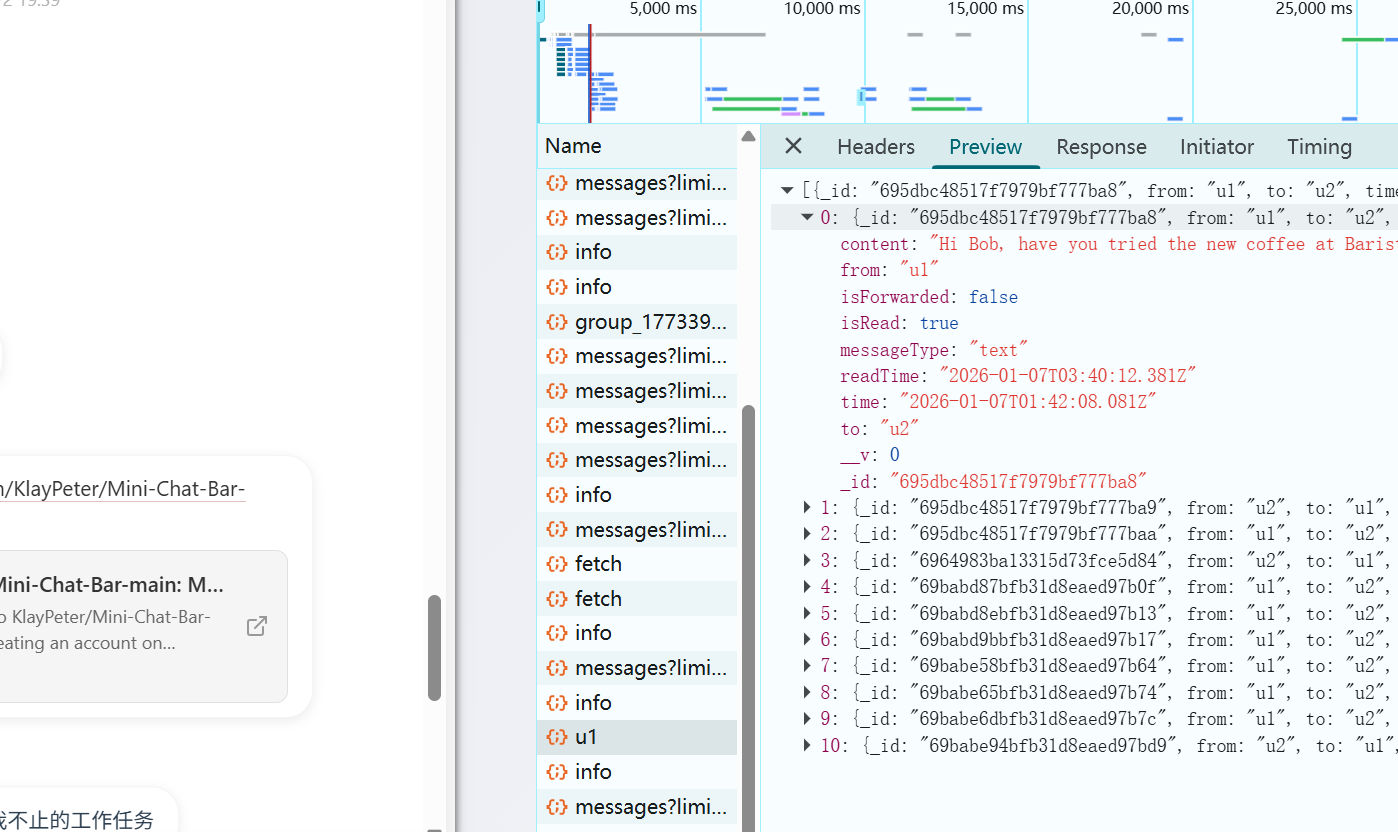
\includegraphics[width=\linewidth,height=4.8cm,keepaspectratio]{img/图6-1_接口返回结果.png}
\caption{接口返回结果}
\end{subfigure}
\hfill
\begin{subfigure}[t]{0.48\textwidth}
\centering
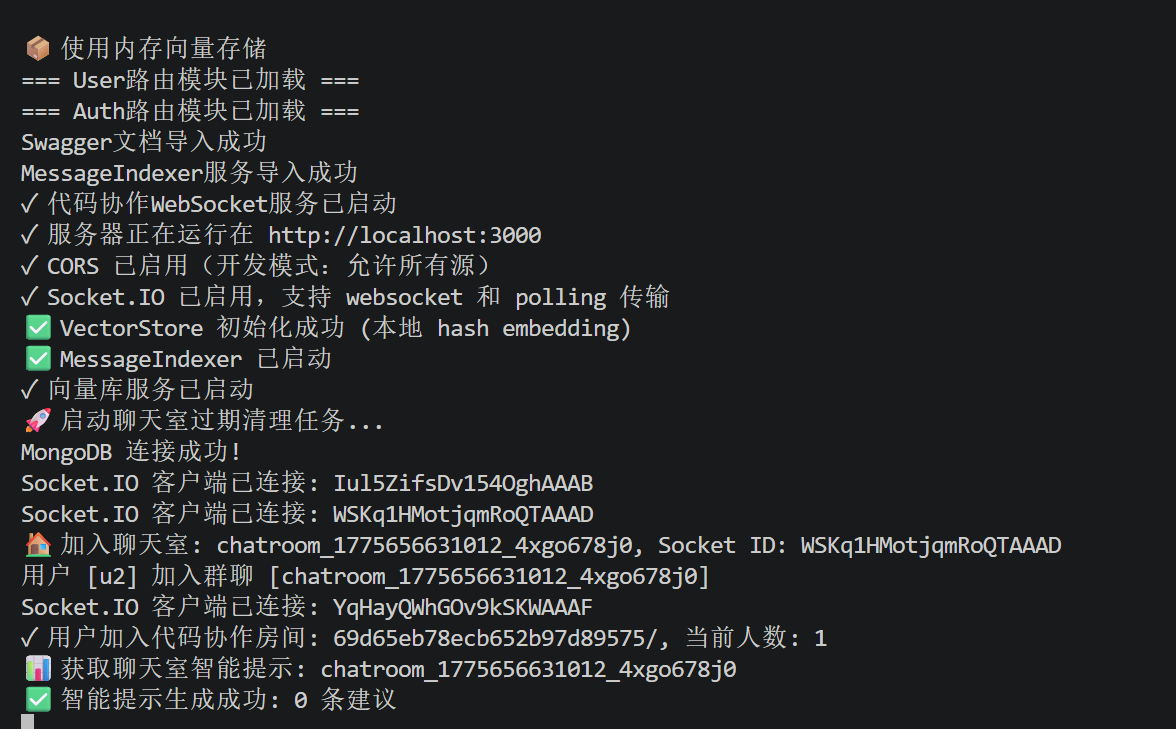
\includegraphics[width=\linewidth,height=4.8cm,keepaspectratio]{img/图6-1_后端终端输出.png}
\caption{后端终端输出}
\end{subfigure}

\vspace{0.6em}

\begin{subfigure}[t]{0.48\textwidth}
\centering
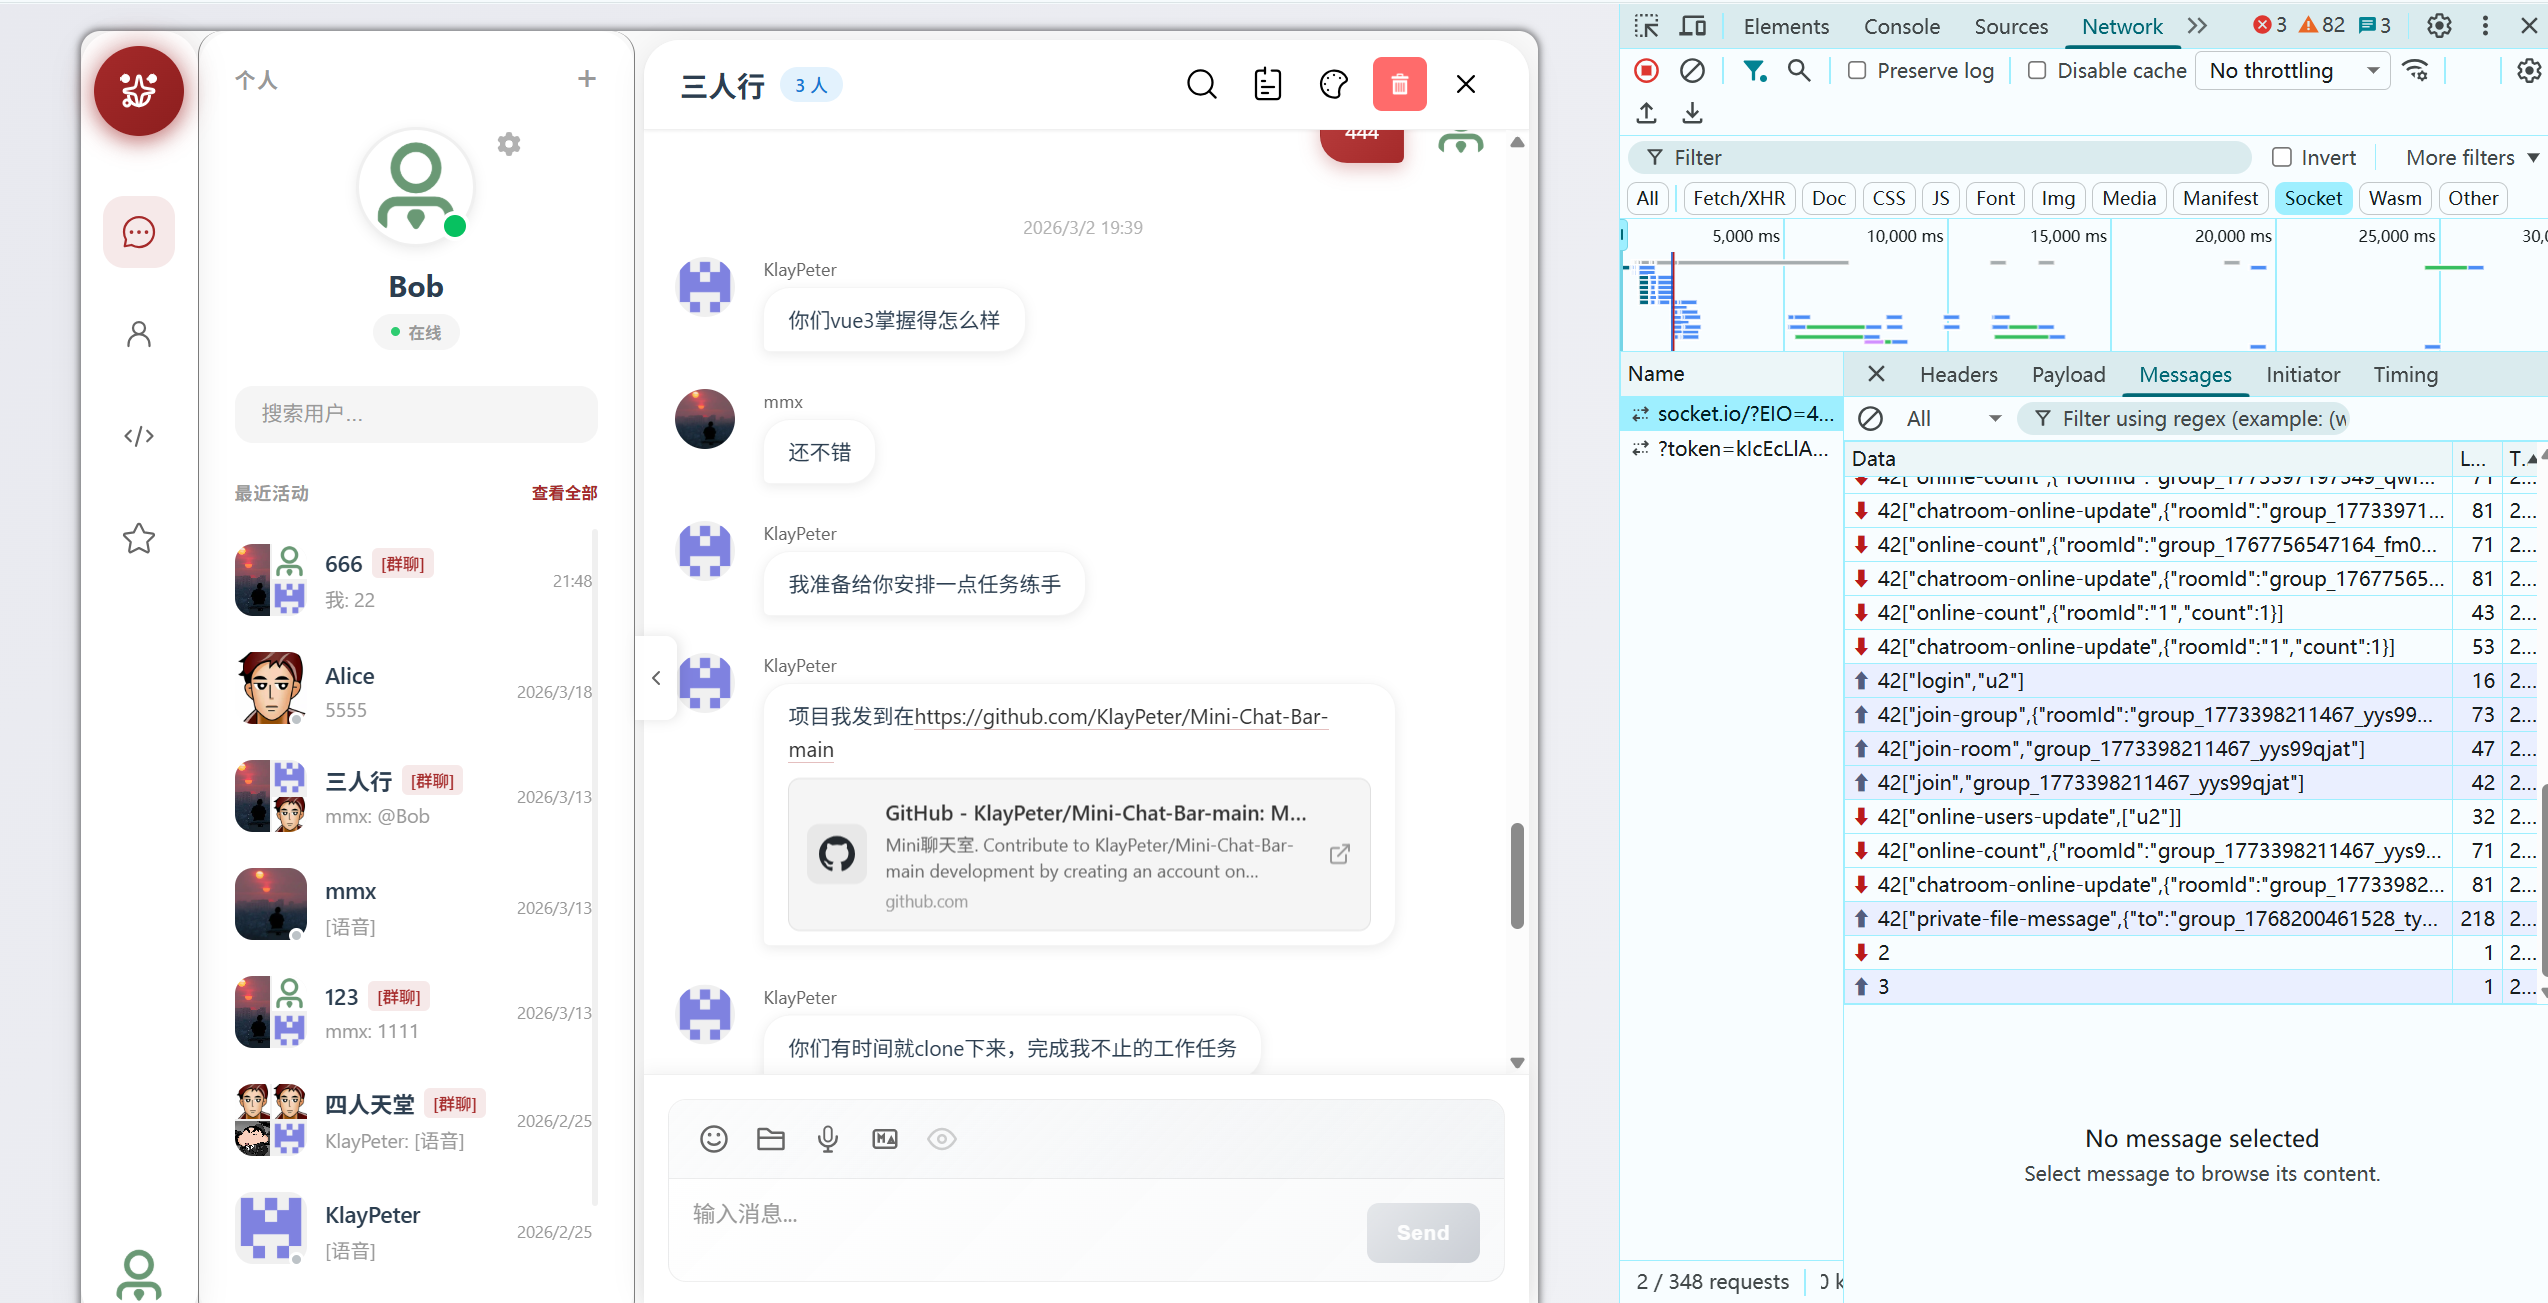
\includegraphics[width=\linewidth,height=4.8cm,keepaspectratio]{img/图6-1_Socket通信记录.png}
\caption{Socket 通信记录}
\end{subfigure}
\hfill
\begin{subfigure}[t]{0.48\textwidth}
\centering
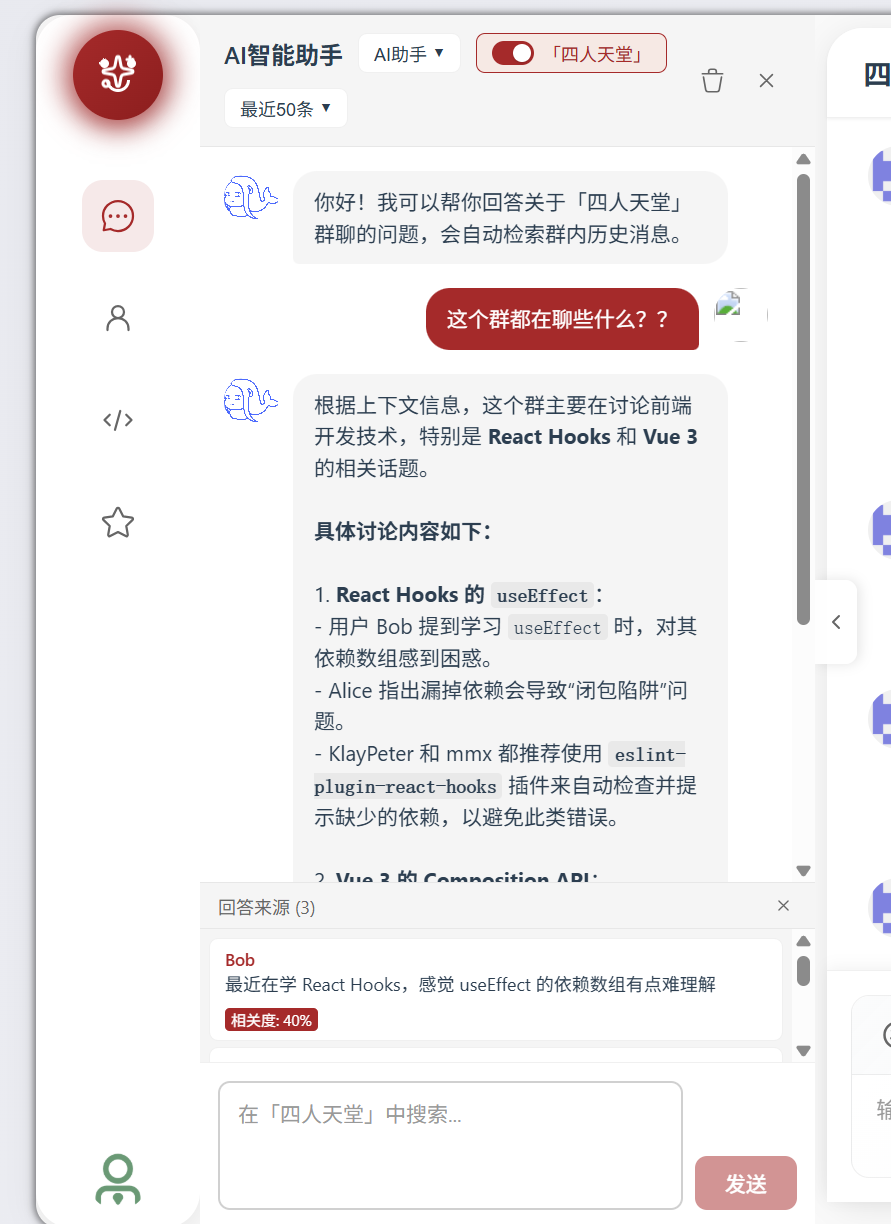
\includegraphics[width=\linewidth,height=4.8cm,keepaspectratio]{img/图6-1_AI返回结果.png}
\caption{AI 返回结果}
\end{subfigure}
\caption{接口与实时通信测试证据组合图}
\label{fig:6-1}
\end{figure}
\FloatBarrier

从表~\ref{tab:6-2} 和图~\ref{fig:6-1} 可以看出，登录、资料读取、聊天室消息写入和私聊事件投递都已跑通。本地环境下 \texttt{private-message} 接收时延约为 6ms；AI 问答接口能够返回完整结果，但耗时明显高于普通业务接口。

\subsection{Web端功能测试}

\subsubsection{登录与会话保持测试}

Web 端先从登录和会话保持开始验证，因为后续所有页面都依赖这条链路。测试覆盖密码登录、验证码登录、会话保持、错误凭证拦截和未登录路由保护。实测显示，登录后可从 \texttt{/login} 跳转至 \texttt{/chats} 并写入本地会话，刷新后仍能保持登录态；清空本地信息后访问受保护路由会重新跳回登录页，见表~\ref{tab:6-3}。

\renewcommand{\arraystretch}{1.08}
\setlength{\tabcolsep}{0.55ex}
\small
\begin{longtable}{M{0.12\textwidth}p{0.16\textwidth}p{0.18\textwidth}p{0.18\textwidth}p{0.23\textwidth}}
\testcaselongtablehead{Web端登录功能测试用例}{tab:6-3}
WEB-01 & 密码登录 & 在登录页输入邮箱和密码并提交 & 页面跳转到主聊天界面，显示当前用户信息 & 登录成功，主界面正常显示，接口耗时与接口测试结果一致 \\
WEB-02 & 验证码登录 & 请求验证码后输入正确验证码并提交 & 登录成功并建立本地会话 & 验证码发送成功，60s 倒计时正常，登录后完成页面跳转 \\
WEB-03 & 会话保持 & 刷新浏览器页面并重新访问主界面 & 路由守卫识别到有效 Token，不跳回登录页 & 刷新后仍停留在主界面，会话保持正常 \\
WEB-04 & 错误凭证拦截 & 输入错误密码后提交表单 & 登录失败并给出错误提示，不进入系统主页 & 页面弹出密码错误提示，未发生错误跳转 \\
WEB-05 & 空表单校验 & 不输入邮箱或密码直接点击登录 & 前端给出必填提示，不发起无效登录流程 & 页面提示“请输入邮箱和密码”，未进入成功登录流程 \\
WEB-06 & 未登录路由拦截 & 直接访问收藏页或聊天室页等受保护路径 & 自动跳转回登录页并清除残留本地数据 & 访问受保护路由时立即跳转至 \texttt{/login}，残留本地数据被清理 \\
\end{longtable}
\normalsize
\FloatBarrier

这一部分重点记录了本地存储、页面跳转和路由守卫状态，相关证据统一汇总到图~\ref{fig:6-2}。测试结果说明登录页、路由守卫和本地会话保持都已正常工作，错误凭证和空表单也会被前端拦截，没有出现异常跳转。

\subsubsection{聊天与聊天室功能测试}

聊天与聊天室测试直接围绕当前前端界面展开，验证对象包括 \texttt{Chat\-View.vue}、\texttt{Con\-tent.vue}、\texttt{ChatRoom\-List\-Panel.vue} 和 \texttt{ChatRoom\-Detail.vue}。这一部分重点检查消息是否写库、历史记录是否能回读、房间是否能正常创建和加入，见表~\ref{tab:6-4}。

\renewcommand{\arraystretch}{1.08}
\setlength{\tabcolsep}{0.55ex}
\small
\begin{longtable}{M{0.12\textwidth}p{0.16\textwidth}p{0.18\textwidth}p{0.18\textwidth}p{0.23\textwidth}}
\testcaselongtablehead{Web端聊天与聊天室功能测试用例}{tab:6-4}
WEB-07 & 私聊消息发送 & 在聊天界面选择联系人并发送文本消息 & 对话区新增消息，后端保存对应私聊记录 & 消息即时回显，数据库中生成对应私聊记录 \\
WEB-08 & 私聊历史回读 & 重新进入会话或刷新页面后加载消息列表 & 能读取历史消息并按时间顺序显示 & 刷新后历史消息正常加载，最新消息位于列表末尾 \\
WEB-09 & 创建公开技术聊天室 & 在聊天室页填写房间名称、技术方向和公开加入方式后提交 & 生成新聊天室并自动出现在房间列表中 & 测试房间创建成功，列表基础回读时可见新建房间 \\
WEB-10 & 加入密码聊天室 & 在聊天室列表中选择目标房间并输入密码加入 & 加入成功并看到历史消息或系统加入提示 & 输入正确密码后成功进入房间，并生成加入系统消息 \\
WEB-11 & 聊天室消息显示与空消息拦截 & 分别发送正常文本和仅空格内容 & 正常消息成功显示，空消息被拦截不提交 & 文本消息正常显示，空白输入不会触发发送，消息顺序一致 \\
\end{longtable}
\normalsize
\FloatBarrier

测试过程中补充记录了私聊回读、公开聊天室创建、密码房间加入和空消息拦截四条关键路径，相关证据统一汇总到图~\ref{fig:6-2}。结果显示，私聊发送、历史回读、公开房间创建和密码房间加入都能正常完成，空白消息也会在前端被拦截，没有进入后端链路。

\subsubsection{AI问答与总结功能测试}

AI 功能测试主要检查三条链路：聊天室内直接提问、输入 \texttt{@AI} 的快捷提问，以及讨论总结生成。为保证结果可重复，测试前先向房间写入 4 条样本消息。实测 AI 问答约 19.5s、总结约 11.8s，刷新后回复仍可回读，见表~\ref{tab:6-5}。

\renewcommand{\arraystretch}{1.08}
\setlength{\tabcolsep}{0.55ex}
\small
\begin{longtable}{M{0.12\textwidth}p{0.16\textwidth}p{0.18\textwidth}p{0.18\textwidth}p{0.23\textwidth}}
\testcaselongtablehead{Web端AI功能测试用例}{tab:6-5}
WEB-12 & AI 问答 & 在聊天室中提交技术问题并等待返回 & 页面显示思考状态，随后插入 AI 回复消息 & AI 接口调用成功，约 19.5s 后返回约 1500 字回复，页面可继续交互 \\
WEB-13 & 讨论总结 & 打开总结对话框并触发总结生成 & 返回结构化总结内容，能够概括主要讨论点 & 总结生成成功，耗时约 11.8s，基于 5 条消息生成约 600 字摘要 \\
WEB-14 & \texttt{@AI} 快捷提问 & 在输入框中插入 \texttt{@AI} 前缀问题并发送 & 自动触发 AI 问答并在消息区追加回复 & 输入 \texttt{@AI} 后先写入用户问题，再生成 AI 回复，流程闭环正常 \\
WEB-15 & 低语料场景问答 & 提交一个与当前技术方向相关的问题 & 仍能返回有效回答，不因历史消息较少而报错 & 样本消息较少时仍返回有效回答，但历史来源列表为 0 \\
WEB-16 & AI 回复持久化 & 刷新聊天室详情页并重新拉取消息 & AI 回复仍可从历史消息中读取并显示 & 刷新后 AI 回复仍可从历史消息中读取，说明结果已成功落库 \\
\end{longtable}
\normalsize
\FloatBarrier

测试中补充记录了从提交问题到结果落库的全过程，相关证据统一汇总到图~\ref{fig:6-2}。从测试结果看，AI 问答、\texttt{@AI} 快捷提问和总结生成都已跑通，且 AI 回复会落库，刷新后仍能回读。当前主要限制仍是耗时受外部模型服务影响，低语料场景下历史来源列表也可能为空。

\subsubsection{收藏功能测试}

收藏测试围绕添加收藏、状态同步、列表回读、取消收藏和组合筛选展开。该模块与消息列表和聊天室状态都有联动，因此除了接口返回，还需要观察前端回显是否正确。基础收藏与回读均正常，但一次带 \texttt{messageType=chatroom} 与关键字的组合查询返回了 500 状态码，见表~\ref{tab:6-6}。

\renewcommand{\arraystretch}{1.08}
\setlength{\tabcolsep}{0.55ex}
\small
\begin{longtable}{M{0.12\textwidth}p{0.16\textwidth}p{0.18\textwidth}p{0.18\textwidth}p{0.23\textwidth}}
\testcaselongtablehead{Web端收藏功能测试用例}{tab:6-6}
WEB-17 & 添加收藏 & 对目标消息执行收藏操作 & 收藏成功，生成消息快照和标签备注信息 & 收藏接口调用成功，消息被写入收藏集合 \\
WEB-18 & 收藏状态同步 & 观察消息右键菜单或收藏状态标记 & 已收藏消息能够被正确识别与回显 & 返回消息区后星标状态正确，重新进入聊天室仍能识别已收藏消息 \\
WEB-19 & 收藏列表回读 & 进入收藏页读取默认列表 & 能看到刚收藏的消息记录及来源信息 & 基础列表查询返回 1 条记录，能够显示测试消息 \\
WEB-20 & 取消收藏 & 在收藏详情页点击“取消收藏”并刷新列表 & 收藏记录被删除，消息恢复未收藏状态 & 取消后收藏页记录消失，聊天室中的收藏状态同步取消 \\
WEB-21 & 收藏组合筛选 & 在收藏页同时使用会话类型和关键字进行筛选 & 正常返回匹配记录 & 一次组合查询返回 500 状态码，说明筛选逻辑仍需进一步校验 \\
\end{longtable}
\normalsize
\FloatBarrier

收藏测试重点记录了“收藏动作触发 - 列表回读 - 状态回显 - 取消收藏 - 组合筛选异常”这一闭环，代表性画面统一汇总到图~\ref{fig:6-2}。其中，聊天室代码协作测试界面对应前端多消息与代码块混排场景，AI 问答结果和讨论总结结果分别对应本节的 WEB-12 至 WEB-16 测试项，设置与主题切换回显则用于补充说明前端交互状态在功能测试过程中的一致性。常规路径已经可用：消息收藏后能在收藏页读到，也能正确取消。问题出现在组合筛选，带 \texttt{messageType=chatroom} 和关键字的查询仍然返回 500，这部分还需要单独排查。

\begin{figure}[H]
\centering
\begin{subfigure}[t]{0.48\textwidth}
\centering
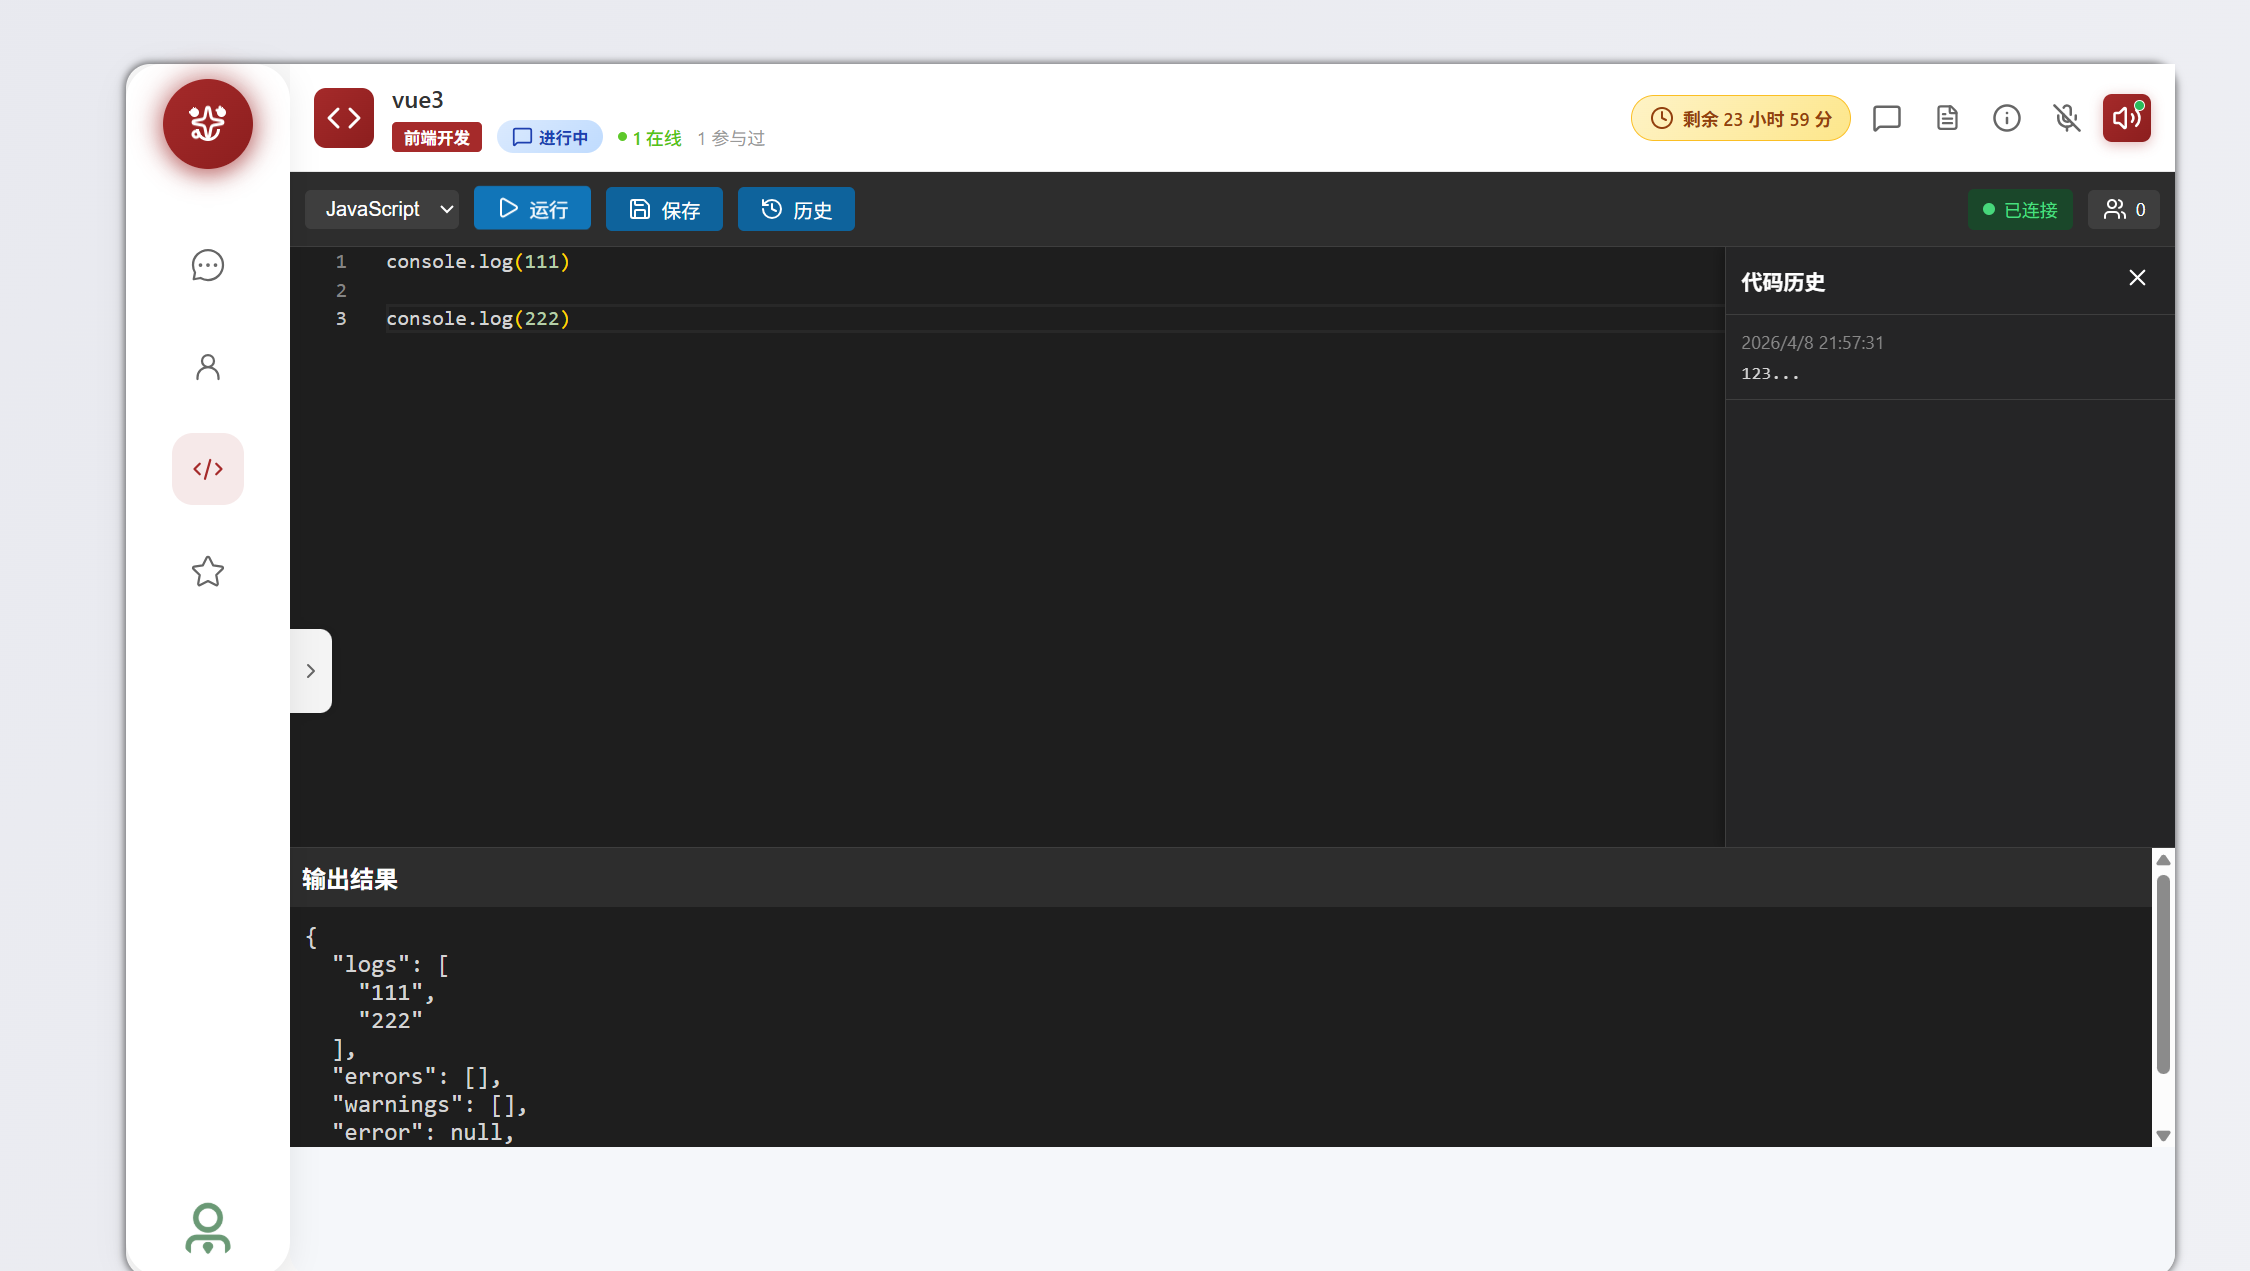
\includegraphics[width=\linewidth,height=4.8cm,keepaspectratio]{img/图6-2_聊天室代码协作测试.png}
\caption{聊天室代码协作测试}
\end{subfigure}
\hfill
\begin{subfigure}[t]{0.48\textwidth}
\centering
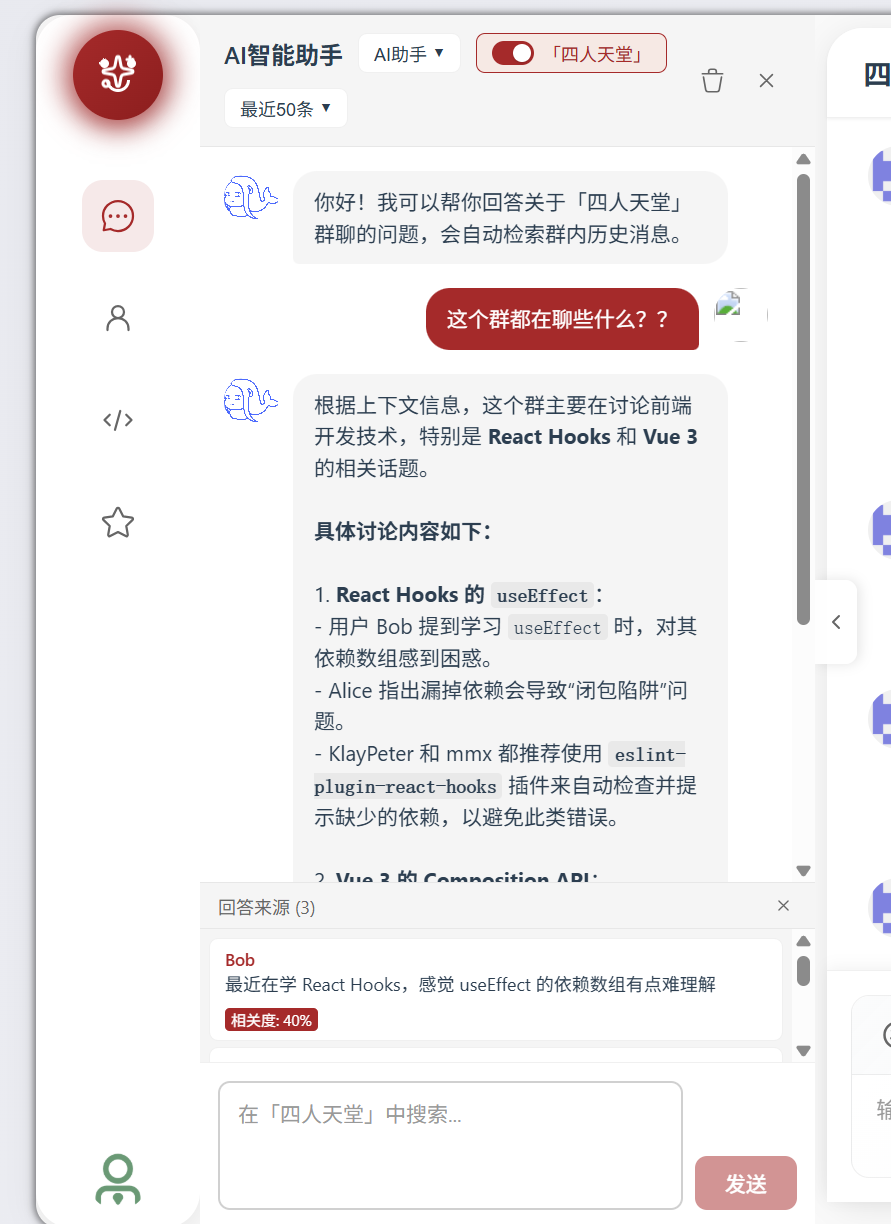
\includegraphics[width=\linewidth,height=4.8cm,keepaspectratio]{img/图6-2_AI问答结果.png}
\caption{AI 问答结果}
\end{subfigure}

\vspace{0.6em}

\begin{subfigure}[t]{0.48\textwidth}
\centering
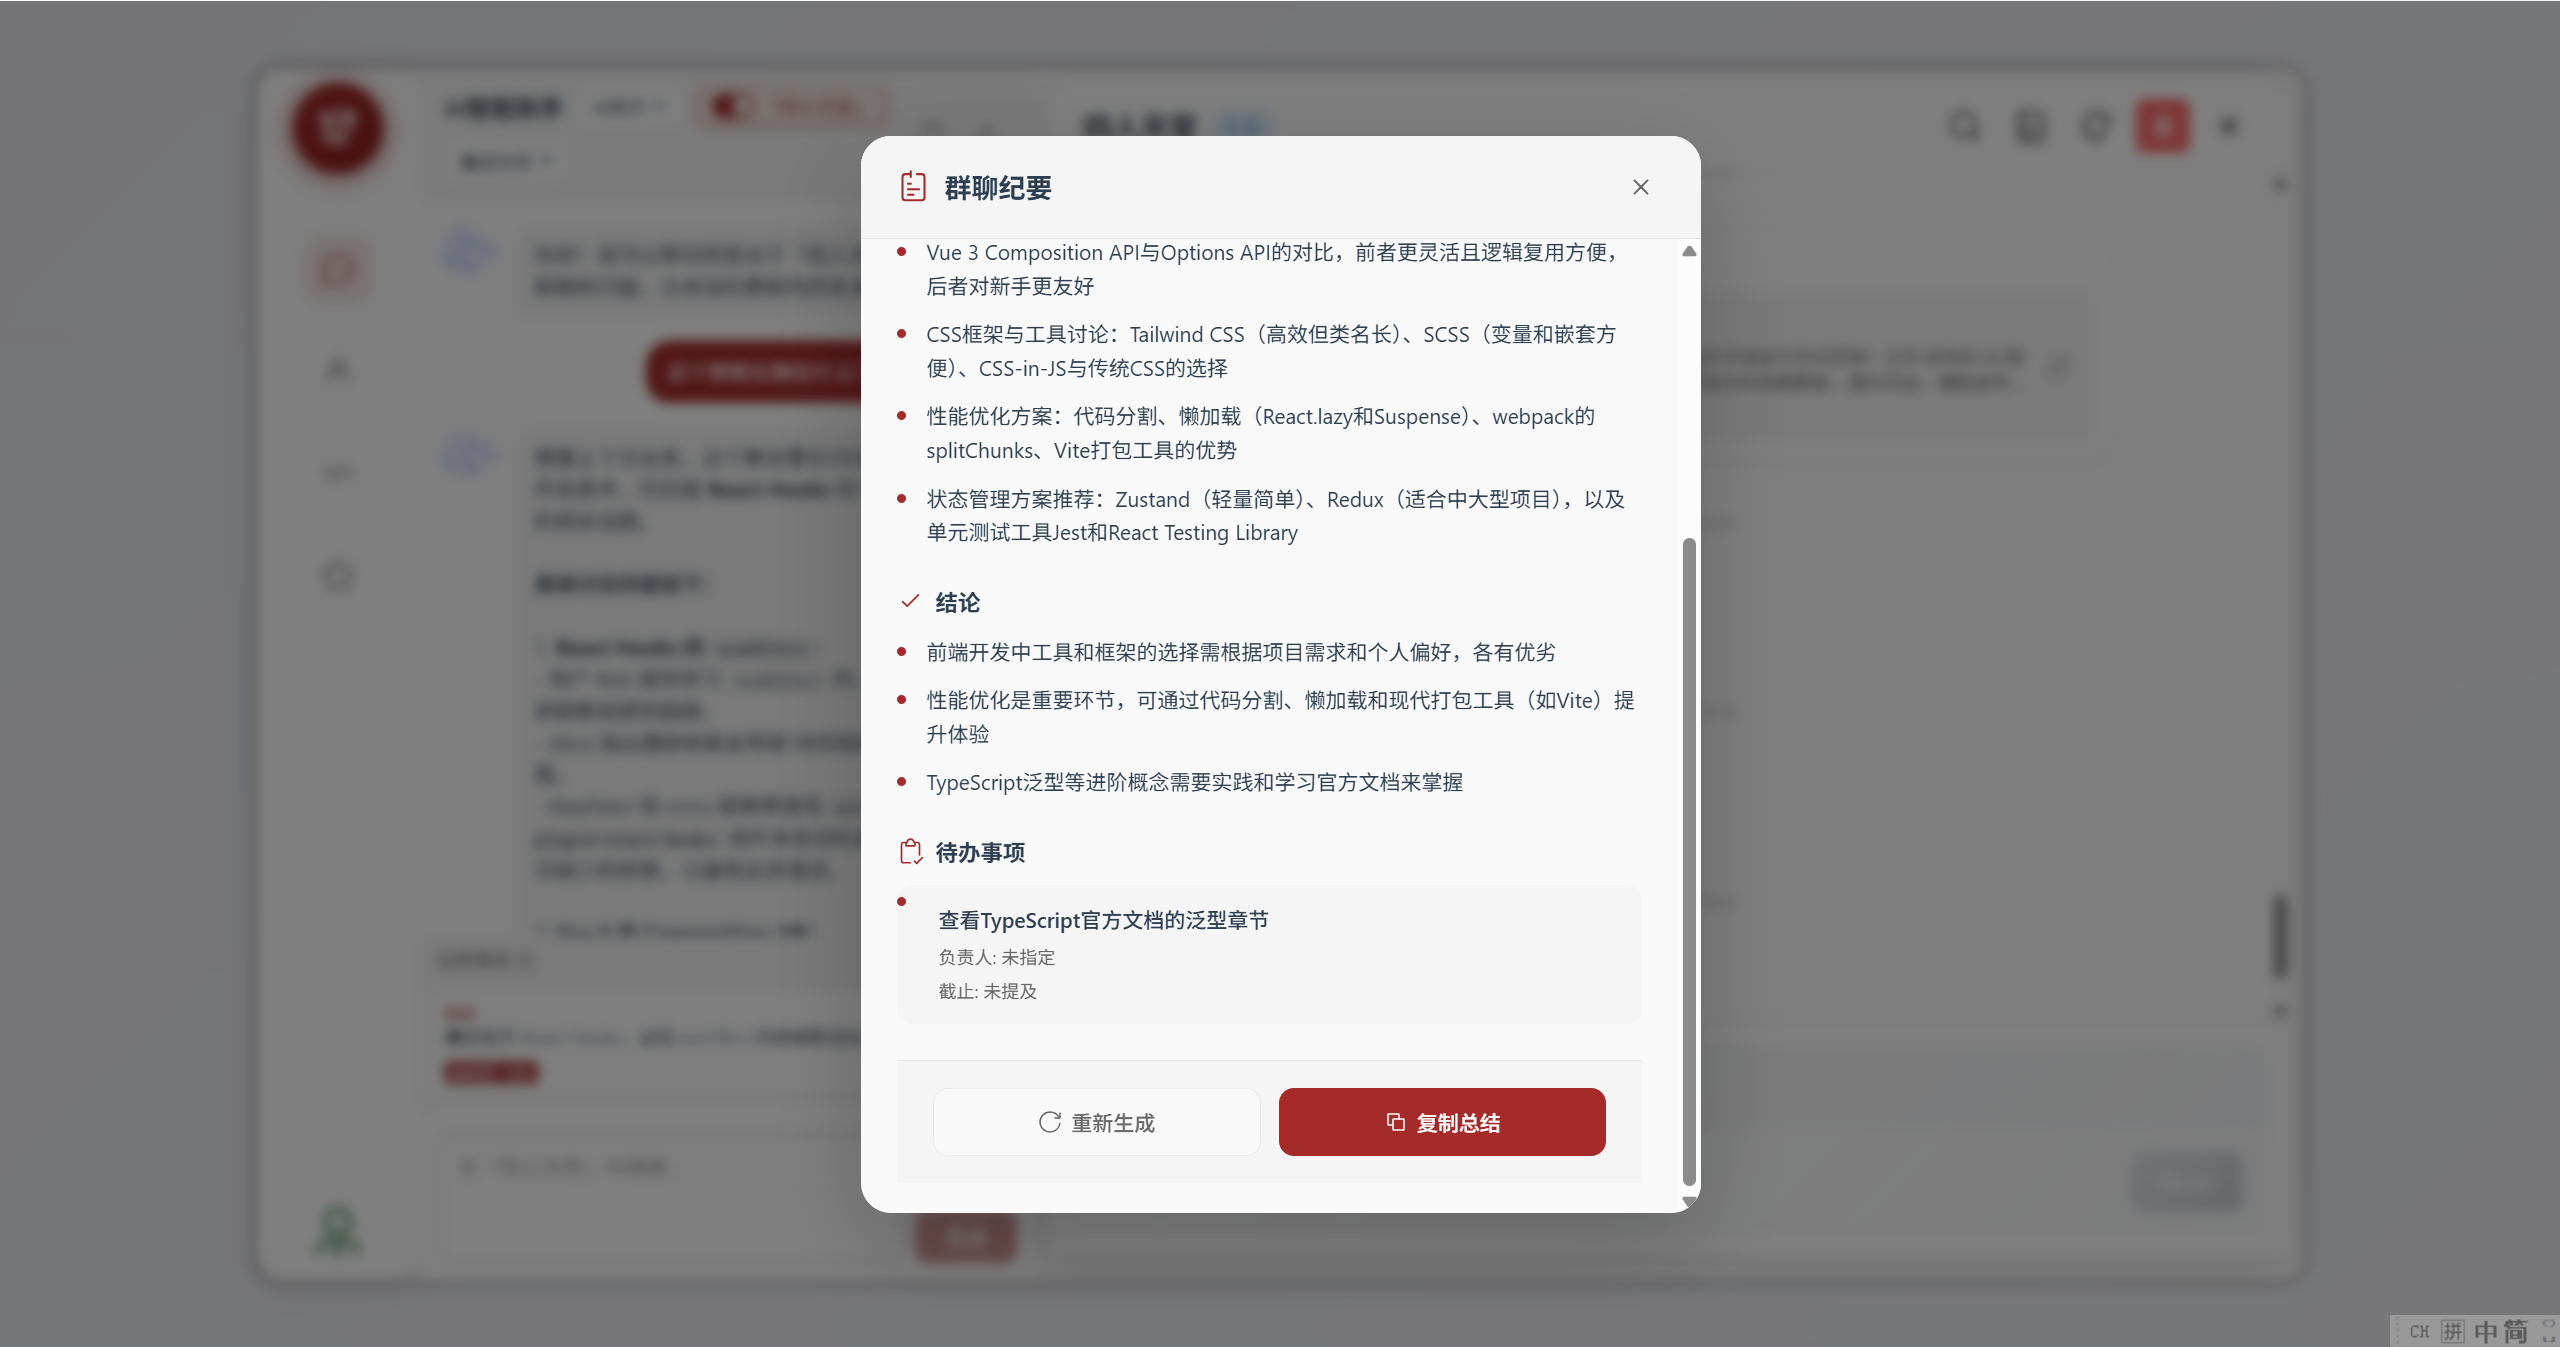
\includegraphics[width=\linewidth,height=4.8cm,keepaspectratio]{img/图6-2_讨论总结结果.png}
\caption{讨论总结结果}
\end{subfigure}
\hfill
\begin{subfigure}[t]{0.48\textwidth}
\centering
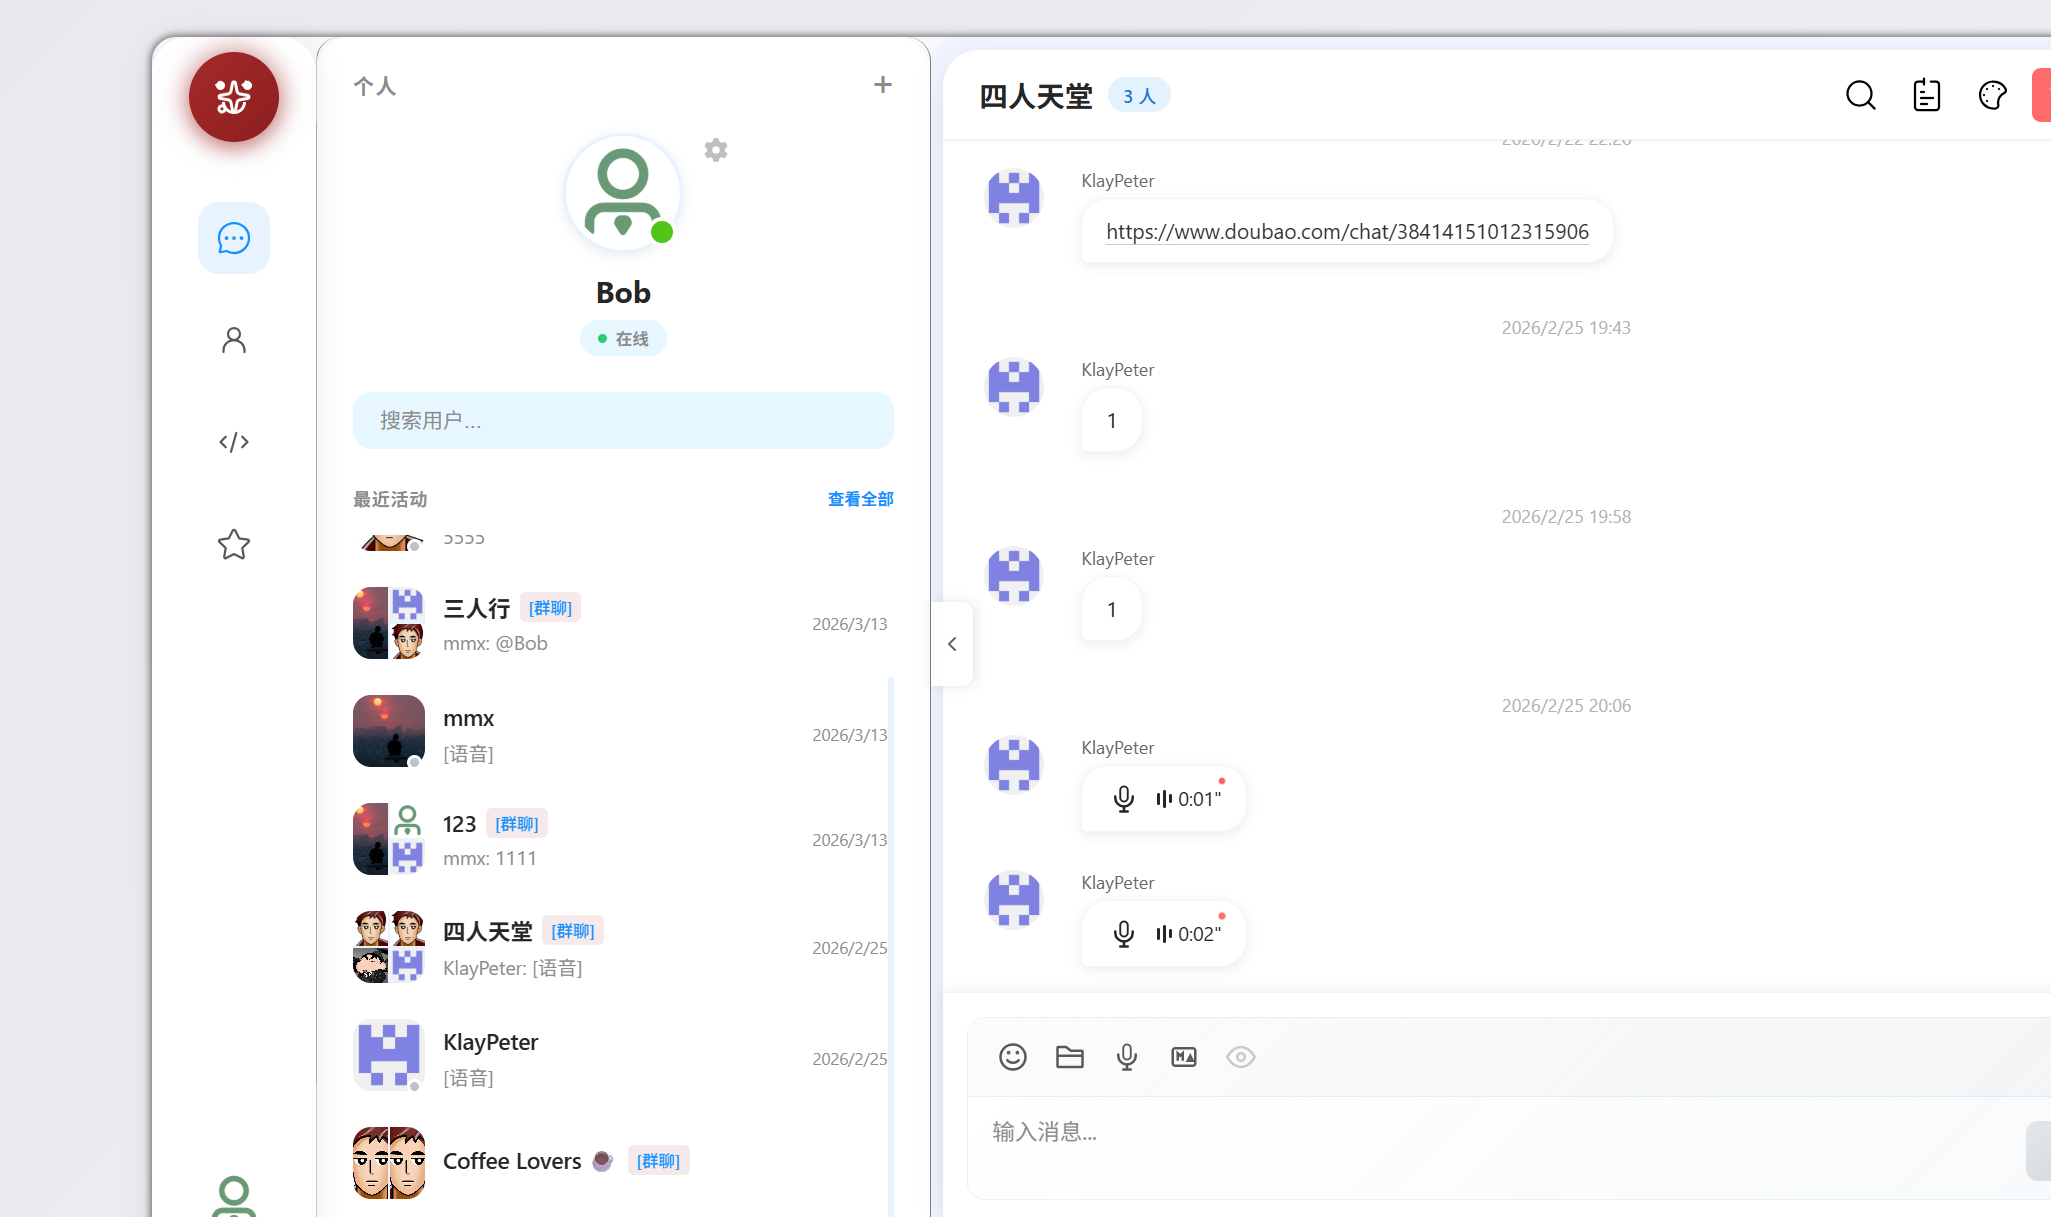
\includegraphics[width=\linewidth,height=4.8cm,keepaspectratio]{img/图6-2_设置与主题切换回显.png}
\caption{设置与主题切换回显}
\end{subfigure}
\caption{Web端功能测试证据组合图}
\label{fig:6-2}
\end{figure}
\FloatBarrier

Web 端功能测试说明，登录、聊天、聊天室、AI 和收藏的主链路已经跑通，但收藏复杂筛选仍然是不稳定点。

\subsection{桌面端功能测试}

桌面端测试以 Windows 打包程序为对象，重点不是重新验证一遍所有功能，而是确认 Web 主链路迁移到 Electron 后仍可用，同时检查托盘、角标、预览和点击跳转这些桌面端特有能力，见表~\ref{tab:6-7}。

\renewcommand{\arraystretch}{1.08}
\setlength{\tabcolsep}{0.55ex}
\small
\begin{longtable}{M{0.12\textwidth}p{0.16\textwidth}p{0.18\textwidth}p{0.18\textwidth}p{0.23\textwidth}}
\testcaselongtablehead{桌面端功能测试用例}{tab:6-7}
DESK-01 & 桌面端启动与登录 & 启动 \texttt{Mini Chat Bar.exe} 并完成登录 & 主窗口正常加载，登录后进入聊天主界面 & 程序可正常启动，登录流程与 Web 端一致 \\
DESK-02 & 托盘驻留 & 点击关闭按钮观察程序行为 & 窗口隐藏到托盘而不是直接退出程序 & 主窗口按设计隐藏，托盘图标仍可保留程序入口 \\
DESK-03 & 未读角标与托盘提示更新 & 触发新消息事件并观察任务栏角标与托盘提示变化 & 未读数更新，窗口获得焦点后清空角标 & 任务栏角标和托盘提示均随未读数变化 \\
DESK-04 & 托盘悬停预览 & 鼠标悬停托盘图标并观察预览窗口 & 弹出预览窗口，显示最近未读会话摘要 & 悬停约 300ms 后弹出预览窗，最多展示最近 5 条未读会话 \\
DESK-05 & 预览点击跳转 & 点击预览窗口中的某条未读消息 & 主窗口恢复并定位到目标会话 & 点击预览项后主窗口被唤起，并定位到对应会话 \\
DESK-06 & 焦点恢复与角标清零 & 点击主窗口或让应用重新获得焦点 & 角标被清空，未读状态与界面同步 & 主窗口恢复焦点后角标被清空，未读状态与界面保持一致 \\
\end{longtable}
\normalsize
\FloatBarrier

桌面端部分重点记录了启动、托盘驻留、未读角标变化、悬停预览和点击跳转五个节点。图~\ref{fig:6-3} 聚焦托盘悬停预览与未读提醒效果，能够直接说明 Electron 侧消息提醒联动正常。

\begin{figure}[H]
\centering
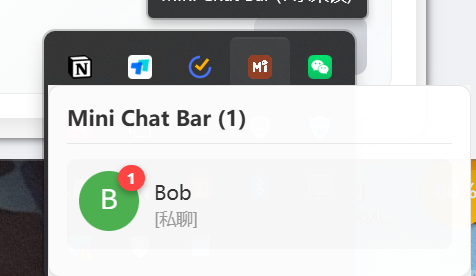
\includegraphics[width=0.46\textwidth]{img/图6-3_桌面端托盘测试.png}
\caption{桌面端功能测试证据图}
\label{fig:6-3}
\end{figure}
\FloatBarrier

结果表明，桌面端已经具备可用的跨端行为：Web 端现有消息链路可以直接复用，托盘提醒和预览跳转也能正常联动。

\subsection{功能测试结果总结}

综合功能测试结果可以认为，当前版本已经跑通了登录、消息、聊天室、AI 和桌面提醒等主要演示链路。当前最明显的问题仍然是收藏组合筛选异常，以及 AI 回答质量受历史语料数量影响。

\section{性能测试}

\subsection{响应时间测试}

性能测试分为响应时间、并发广播和资源占用三部分。响应时间测试先检查日常接口的返回速度，再记录 AI 问答和聊天室总结这类耗时明显更长的调用，量化结果见表~\ref{tab:6-8} 和表~\ref{tab:6-9}。

\renewcommand{\arraystretch}{1.08}
\setlength{\tabcolsep}{0.55ex}
\small
\begin{longtable}{M{0.12\textwidth}p{0.16\textwidth}p{0.18\textwidth}p{0.18\textwidth}p{0.23\textwidth}}
\testcaselongtablehead{响应时间测试用例}{tab:6-8}
PERF-01 & 登录接口响应 & 连续调用登录接口 10 次并记录耗时 & 平均响应时间稳定且无异常失败 & 10 次调用全部成功，平均耗时约 58ms \\
PERF-02 & 用户信息接口响应 & 连续访问用户信息接口 10 次并记录耗时 & 查询接口保持毫秒级返回 & 10 次调用全部成功，平均耗时约 5ms \\
PERF-03 & 聊天室列表接口响应 & 连续访问聊天室列表接口 10 次并记录耗时 & 列表查询稳定返回 & 10 次调用全部成功，平均耗时约 5ms \\
PERF-04 & 消息列表接口响应 & 连续访问消息列表接口 10 次并记录耗时 & 消息读取保持毫秒级返回 & 10 次调用全部成功，平均耗时约 6ms \\
PERF-05 & 收藏列表接口响应 & 连续访问收藏列表接口 10 次并记录耗时 & 收藏页查询稳定返回，不出现超时 & 10 次调用全部成功，平均耗时约 7ms \\
PERF-06 & AI 问答响应 & 调用 AI 问答接口并记录返回时间 & 返回完整回答，不出现超时中断 & 单次耗时约 19.5s，返回约 1500 字内容 \\
PERF-07 & 聊天总结响应 & 调用聊天室总结接口并记录返回时间 & 返回结构化摘要内容 & 单次耗时约 11.8s，基于 5 条消息生成约 600 字摘要 \\
\end{longtable}
\normalsize

\begin{table}[!htbp]
\centering
\caption{响应时间测试结果}
\label{tab:6-9}
\small
\renewcommand{\arraystretch}{1.15}
\setlength{\tabcolsep}{0.8ex}
\begin{tabular}{M{0.20\textwidth}M{0.13\textwidth}M{0.13\textwidth}M{0.13\textwidth}p{0.29\textwidth}}
\toprule
\textbf{测试项} & \textbf{平均值} & \textbf{最小值} & \textbf{最大值} & \textbf{结果分析} \\
\midrule
登录接口 & 58ms & 57ms & 61ms & 认证、密码比对和 JWT 生成均在可接受范围内完成 \\
用户信息接口 & 5ms & 4ms & 6ms & 读取单用户资料开销较小，适合高频调用 \\
聊天室列表接口 & 5ms & 4ms & 7ms & 列表查询结构简单，返回速度稳定 \\
聊天室消息列表接口 & 6.0ms & 5ms & 8ms & 小规模消息分页读取响应平稳 \\
收藏列表接口 & 7ms & 6ms & 9ms & 收藏数量较少时查询稳定，来源名补全未带来明显额外开销 \\
聊天室消息发送接口 & 15ms & -- & -- & 消息写入数据库并广播后仍保持毫秒级返回 \\
私聊消息发送接口 & 11ms & -- & -- & 私聊接口链路较短，返回速度快 \\
私聊 WebSocket 投递 & 6ms & -- & -- & 本地实时消息转发几乎无可感知延迟 \\
AI 问答接口 & 19.5s & -- & -- & 耗时主要来自外部大模型调用，而非本地业务逻辑 \\
聊天室总结接口 & 11.8s & -- & -- & 总结耗时低于 AI 问答，适合阶段性使用而不适合高频触发 \\
\bottomrule
\end{tabular}
\end{table}

\FloatBarrier
表~\ref{tab:6-9} 显示，登录、资料、列表和消息接口都保持在毫秒级；AI 问答约为 19.5s，聊天室总结约为 11.8s。当前性能瓶颈并不在本地 Node 服务，而在外部模型调用。

\subsection{并发性能测试}

并发性能测试主要观察 Socket.IO 在单机环境下的广播表现。测试脚本通过 \texttt{socket.io-client} 建立本地连接，统计平均时延、P95 和最大时延，结果见表~\ref{tab:6-10} 和表~\ref{tab:6-11}。

\renewcommand{\arraystretch}{1.08}
\setlength{\tabcolsep}{0.55ex}
\small
\begin{longtable}{M{0.12\textwidth}p{0.16\textwidth}p{0.18\textwidth}p{0.18\textwidth}p{0.23\textwidth}}
\testcaselongtablehead{并发性能测试用例}{tab:6-10}
CON-01 & 20 客户端广播 & 建立 20 个 Socket 客户端并广播一条群消息 & 所有客户端均能收到消息，广播延迟较低 & 20 个客户端全部收到消息，成功率 100\% \\
CON-02 & 50 客户端广播 & 建立 50 个 Socket 客户端并广播一条群消息 & 所有客户端均能收到消息，不出现掉线 & 50 个客户端全部收到消息，成功率 100\% \\
CON-03 & 100 客户端广播 & 建立 100 个 Socket 客户端并广播一条群消息 & 广播仍能完成，延迟增长保持可控 & 100 个客户端全部收到消息，成功率 100\% \\
CON-04 & 100 客户端连续广播 & 连续发送 10 轮群消息并统计投递情况 & 多轮广播后仍无掉线和明显积压 & 10 轮广播共 1000 次投递均成功，未观察到异常断连 \\
CON-05 & 客户端断线重连后广播 & 广播新消息并观察重连客户端接收情况 & 重连客户端可恢复收消息，在线客户端总数保持稳定 & 重连客户端可再次收到后续广播，房间在线状态恢复正常 \\
\end{longtable}
\normalsize

\begin{table}[!htbp]
\centering
\caption{并发性能测试结果}
\label{tab:6-11}
\small
\renewcommand{\arraystretch}{1.15}
\setlength{\tabcolsep}{0.5ex}
\begin{tabular}{M{0.14\textwidth}M{0.13\textwidth}M{0.13\textwidth}M{0.13\textwidth}M{0.12\textwidth}p{0.20\textwidth}}
\toprule
\textbf{并发客户端数} & \textbf{平均送达时延} & \textbf{P95时延} & \textbf{最大时延} & \textbf{接收成功率} & \textbf{结果分析} \\
\midrule
20 & 3ms & 3ms & 3ms & 100\% & 小规模广播无明显抖动 \\
50 & 3ms & 3ms & 3ms & 100\% & 广播链路稳定，时延未出现明显恶化 \\
100 & 4ms & 5ms & 5ms & 100\% & 单机环境下仍可稳定广播，时延有所上升但整体可控 \\
\bottomrule
\end{tabular}
\end{table}

\FloatBarrier
如图~\ref{fig:6-4}所示，并发广播测试示意图展示了单机环境下 100 客户端广播的主要观测指标。

\begin{figure}[H]
\centering
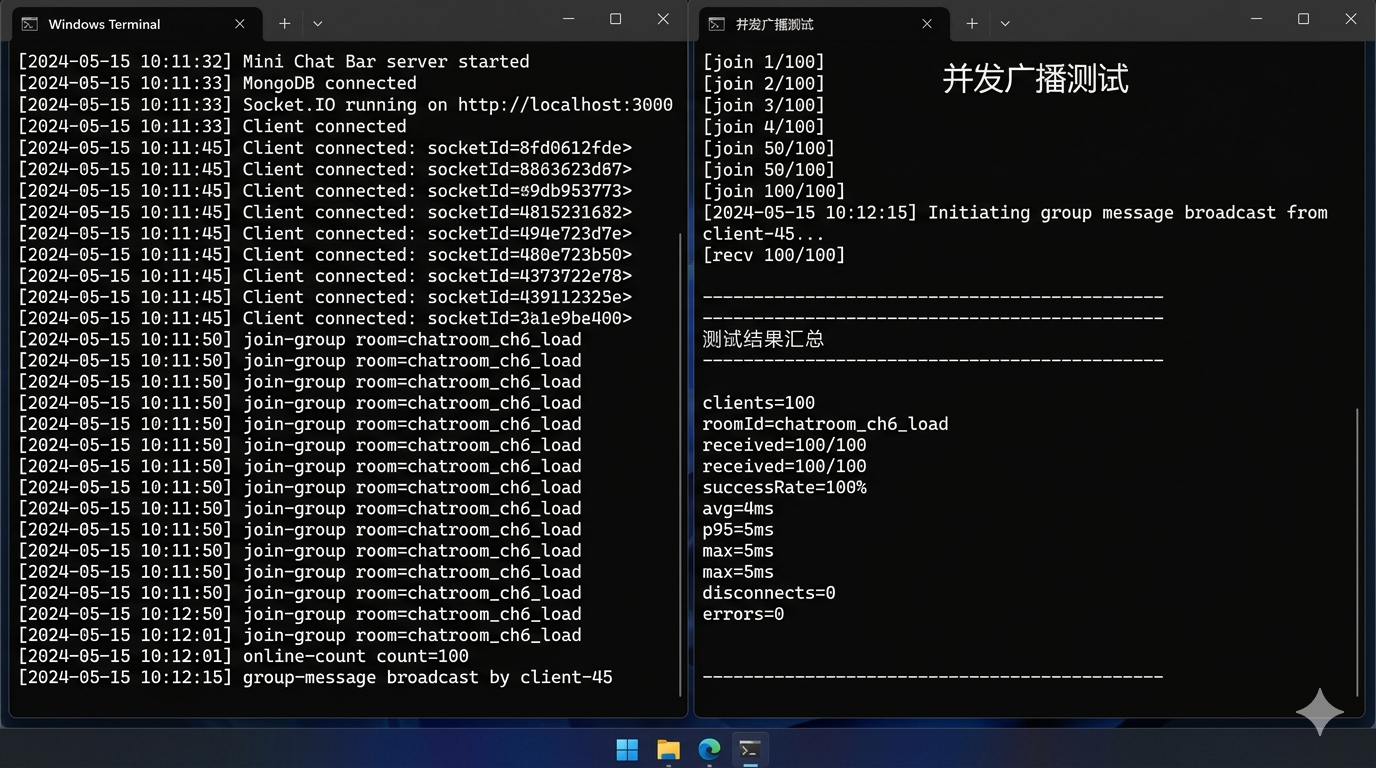
\includegraphics[width=0.92\textwidth]{img/图6-4_并发广播测试日志示意图.png}
\caption{并发广播测试日志示意图}
\label{fig:6-4}
\end{figure}
\FloatBarrier

在 20、50 和 100 个客户端下，广播成功率均为 100\%。单机 100 客户端时平均时延约为 4ms，说明当前规模下广播链路仍然稳定，但这一结果只代表本地环境。

\subsection{资源占用测试}

资源占用测试分别记录 100 客户端广播、单次 AI 问答和单次聊天室总结三种场景下的 CPU 与内存变化，结果见表~\ref{tab:6-12} 和表~\ref{tab:6-13}。

\renewcommand{\arraystretch}{1.08}
\setlength{\tabcolsep}{0.55ex}
\small
\begin{longtable}{M{0.12\textwidth}p{0.16\textwidth}p{0.18\textwidth}p{0.18\textwidth}p{0.23\textwidth}}
\testcaselongtablehead{资源占用测试用例}{tab:6-12}
RES-01 & 广播场景资源占用 & 建立 100 个 Socket 客户端并完成一次群消息广播 & CPU 和内存占用保持在可控范围内，不出现进程异常退出 & 广播测试完成，进程工作集与私有内存均低于 200MB \\
RES-02 & AI 问答场景资源占用 & 对聊天室发起一次完整 AI 问答请求并记录进程占用 & 在等待 AI 返回期间服务进程保持稳定 & AI 请求完成后进程保持正常，内存占用低于 120MB \\
RES-03 & AI 总结场景资源占用 & 对聊天室发起一次完整讨论总结请求并记录进程占用 & 总结生成期间服务进程稳定，无明显资源抖动 & 总结请求完成后进程保持正常，内存占用低于 115MB \\
\end{longtable}
\normalsize

\renewcommand{\arraystretch}{1.15}
\setlength{\tabcolsep}{0.5ex}
\small
\begin{longtable}{M{0.18\textwidth}M{0.12\textwidth}M{0.13\textwidth}M{0.13\textwidth}M{0.13\textwidth}p{0.20\textwidth}}
\resourceusagelongtablehead{资源占用测试结果}{tab:6-13}
100 客户端广播 & 1.5s & 2.1\% & 161MB & 187MB & 连接数增长后内存占用上升，但仍保持在较低水平 \\
单次 AI 问答 & 31.0s & 低于 1\% & 93MB & 118MB & CPU 占用不明显，说明耗时主要消耗在等待外部模型返回 \\
单次 AI 总结 & 12.2s & 低于 1\% & 90MB & 114MB & 与 AI 问答相比总体占用接近，但等待时间更短 \\
\end{longtable}
\normalsize

\FloatBarrier
如图~\ref{fig:6-5}所示，资源占用监测示意图展示了广播压力和 AI 请求压力下的服务端状态差异。

\begin{figure}[H]
\centering
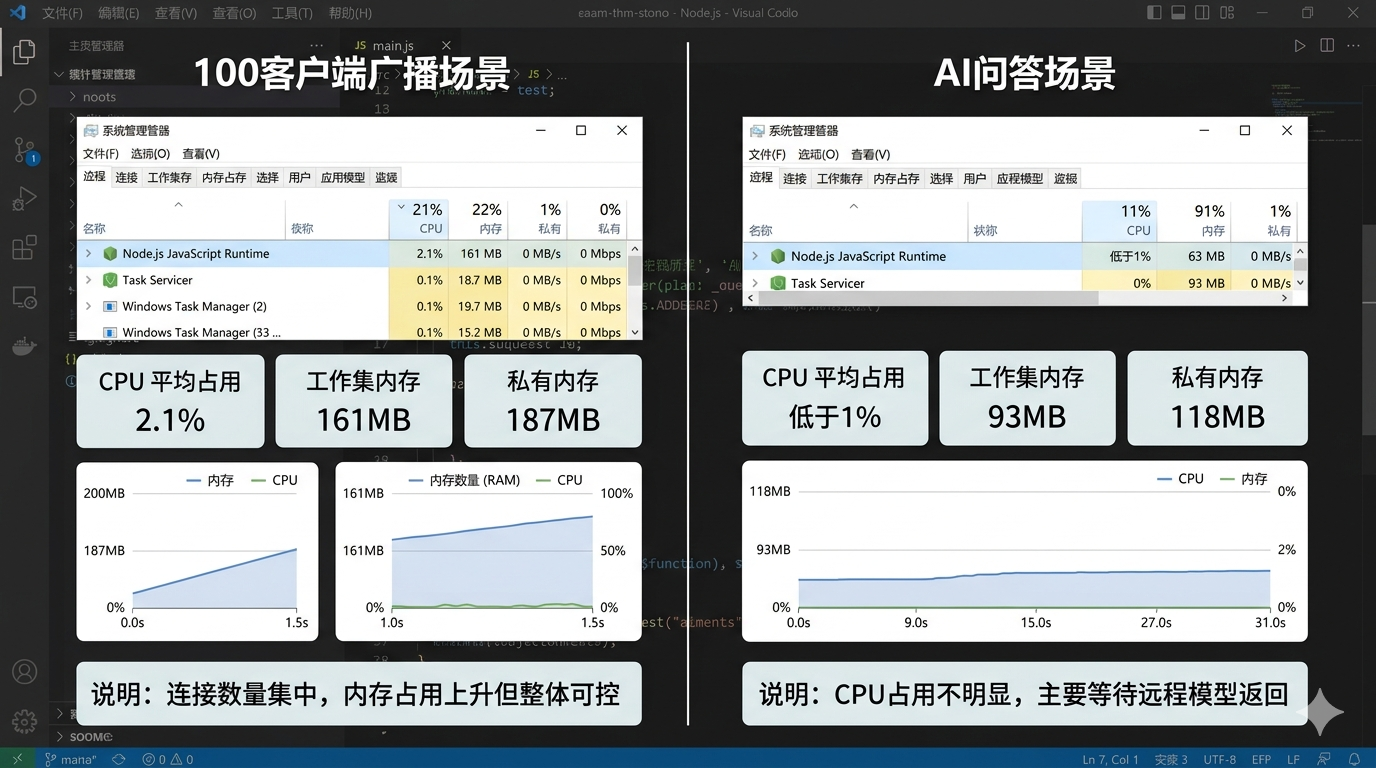
\includegraphics[width=0.92\textwidth]{img/图6-5_资源占用监测示意图.png}
\caption{资源占用监测示意图}
\label{fig:6-5}
\end{figure}
\FloatBarrier

资源监测结果说明，广播场景主要抬高内存占用，AI 场景则更多消耗等待时间。本地服务端 CPU 压力不高，说明 AI 耗时主要来自等待外部模型返回。

\subsection{性能测试结果总结}

综合响应时间、并发广播和资源占用结果，系统在当前单机部署下已经能满足课程项目和答辩演示。普通接口、消息列表读取和 Socket 广播都保持了较稳定的响应水平，说明当前前后端主链路在小规模本地环境下可以支撑连续展示与演示操作。

从性能瓶颈分布看，当前最主要的耗时来源仍然是外部模型调用，而不是本地 Node 服务与数据库访问；从资源曲线看，广播场景主要推高内存占用，AI 场景则更多体现在等待时间拉长。后续需要优先处理的仍是 AI 耗时和收藏复杂筛选这两个边界问题，同时也应继续关注更高并发和更长时段运行下的稳定性变化。

\chapter{总结与展望}

\section{工作总结}

到论文撰写完成时，Mini-Chat-Bar 已经完成了从需求分析、系统设计到实现与测试的主要工作。这个系统面向的不是泛社交聊天，而是技术交流场景里更常见的几条链路：用户登录后可以进入主聊天界面，在私聊和聊天室之间切换；消息支持文本、代码、图片和文件；需要反复回看的内容可以加入收藏；讨论过程中如果需要补充说明或快速整理结论，还可以调用 AI 问答和讨论总结功能。

结合整个毕业设计的推进过程，我完成的工作主要集中在几个连续阶段。前期先梳理需求、确定论文结构，并在此基础上把系统定为前后端分离架构；随后围绕用户、私聊、聊天室、收藏、AI 对话与聊天总结等模块整理业务流程和数据结构；在实现阶段继续完成 Web 端界面、Electron 桌面端适配、后端接口、Socket.IO 实时链路以及 AI 问答与总结功能的联调；最后再把需求分析、系统设计、实现过程和测试结果整理成论文。对我来说，这次毕设不是只把一个功能做出来，而是把分析、设计、编码、测试和文档整理完整地走了一遍。

从当前实现结果看，系统的主要链路已经可以闭环运行。前端已经完成登录、主聊天界面、聊天室详情、收藏页和 AI 面板等核心页面；后端已经完成用户认证、消息处理、聊天室管理、收藏管理和 AI 流式问答等服务；MongoDB 用于保存用户、房间、私聊消息、聊天室消息、收藏和 AI 相关数据。具体到业务流程上，邮箱登录后可以进入 \texttt{ChatView.vue}，私聊通过 \texttt{/api/chat/messages/:id} 与 \texttt{private-message} 联动，聊天室消息通过 \texttt{/room/:roomId/messages} 和 \texttt{group-message} 同步，\texttt{@AI} 提问则通过 \texttt{/api/chatroom-ai/ask-stream} 与 \texttt{ai-stream-chunk} 回写结果。

第六章的测试结果也说明，这套系统已经具备基本的演示和使用条件。普通接口保持毫秒级响应，私聊消息和聊天室消息可以稳定写入并同步，桌面端的托盘驻留、未读提醒和消息预览已经能够正常工作。AI 问答与总结链路虽然明显慢于普通接口，但已经跑通了从提问、检索、生成到结果落库的完整流程。对本科毕业设计而言，系统已经完成了预期的主要目标。

与本课题实施过程相关的任务书、开题/中期检查、指导记录、审批表和成绩评定等材料，已统一整理于\hyperref[app:materials]{附录}。

\section{实践体会}

这次毕业设计让我更直接地体会到，聊天系统真正难的地方往往不在某一个页面或者某一个接口本身，而在于多条链路同时工作时能不能保持一致。私聊和聊天室都不是前端把消息回显出来就算结束，还要继续确认消息有没有写入数据库、Socket 有没有及时推送、刷新页面后历史记录能不能重新读回来。桌面端提醒也是同样的问题，弹出通知只是最表面的结果，后面还牵涉未读数、托盘状态和窗口焦点变化。如果只看单独一个点，很多问题都不算复杂；放到完整系统里之后，前后端联动和状态同步的影响就会一起出现。

另一个比较深的体会来自 AI 模块。开始做之前，很容易把它理解成“接入一个模型接口”，真正落到系统里才发现关键并不只在模型返回内容本身，而在于历史消息有没有进入索引、检索结果能不能贴近当前讨论、AI 回复生成后能不能继续以普通消息的形式保存和回看。聊天室里的 \texttt{@AI} 不是一个孤立入口，它必须和现有消息流共存，这一点和对话历史管理型问答系统强调的上下文连续性是一致的\cite{historyragqa2026}。这一部分做完以后，我对 AI 接入业务系统的认识比之前具体得多，也更清楚模型能力、消息数据和场景设计之间是如何互相影响的。

从个人收获来看，这次毕设最大的价值在于把一个完整项目真正从头做到尾。以往课程作业通常围绕单个功能展开，范围比较有限；这次需要同时考虑需求分析、系统设计、代码实现、测试验证和结果说明。做完整个过程后，我对接口设计、实时通信、数据库建模、前端状态管理以及问题定位都有了更直观的认识，这些经验比单独完成某一页界面更有价值。

\section{系统不足与展望}

当前版本已经能够支撑课程项目演示和小规模使用，但距离长期稳定运行的技术交流平台还有明显差距。首先，系统目前主要在本地和单机环境下开发与测试，更适合原型验证。如果后续用户数量继续增加，服务端在并发连接、消息广播和 AI 请求调度上的压力会更明显。下一步如果继续扩展，部署方式、缓存机制和服务拆分都需要重新考虑。

其次，AI 模块虽然已经跑通了问答和总结的基本链路，但它对历史语料数量和检索结果质量依赖较强。当聊天室消息较少，或者检索结果不够准确时，回答仍然会偏通用；长上下文利用效率不稳定时，这个问题还会更明显\cite{longcontext2024}。后续更值得投入的方向，不是单纯再换一个模型，而是继续优化消息索引、检索排序和上下文拼接策略，让 AI 返回内容更贴近房间里的真实讨论\cite{ragllmsurvey2024}。即便模型能力继续扩展，大语言模型在业务系统中的稳定性和可控性仍然需要长期处理\cite{llmsurvey2023}。

再次，系统在稳定性方面还有需要补强的地方。第六章测试已经发现，收藏模块在组合筛选条件下仍会出现 500 错误。这说明主路径虽然已经跑通，但复杂路径下的异常处理还不够扎实。相比继续叠加新功能，后续更应该优先补上异常处理、回归测试和日志分析，把现有链路先做稳。

最后，从产品方向看，当前系统已经覆盖了聊天、收藏和 AI 辅助三条主线，但对技术团队更深层次的协作支持还不够。例如，多人代码协同、任务跟踪、知识归档的结构化整理等能力，目前还没有形成完整方案。后续如果继续推进，可以在保持轻量化的前提下逐步补充这些能力，使系统从“技术讨论工具”进一步发展为“面向技术交流的协作平台”。

总体来看，Mini-Chat-Bar 已经验证了一个比较清楚的方向：技术交流系统不应只负责消息传递，还应支持历史回看、结果沉淀和适度的 AI 辅助。当前版本还算不上成熟产品，但主框架已经建立起来，后续只要继续围绕稳定性、检索质量和协作深度推进，系统仍然有较大的完善空间。


\bibliography{bibHzu}

\chapterspecialcenter{致 谢}
行文至此，这篇论文也接近尾声，大学四年的时光仿佛也在这一页页文字里慢慢落定。回望从选题、设计、实现到反复修改的过程，我并不是独自走到这里。一路上，老师的指引、同学的陪伴与帮助，让许多原本紧张而忙碌的时刻，都多了几分踏实与从容。

衷心感谢我的指导老师刘利副教授，在论文选题、系统设计和写作修改过程中给予我耐心而细致的指导。老师严谨认真的治学态度，也让我明白，完成毕业设计不仅是完成一项任务，更是学着把问题想清楚、把事情做扎实。

同时，也感谢身边的同学和朋友。在系统开发和论文撰写过程中，大家陪我一起讨论思路、排查问题、完善细节。许多看似平常的交流与提醒，都会在回头看时显出分量，它们像夜里一直亮着的灯，让这段毕业时光不只是匆忙，也留下了温度。

在此，向所有曾给予我帮助、鼓励与关心的老师、同学和朋友，致以真诚的谢意。那些一起思考、一起赶进度、一起把问题慢慢解决的日子，也会成为我大学生活中很珍贵的一部分。

\clearpage
\appendixspecialcenter{附录}

本附录 A 至附录 I 主要对应第 5 章“系统实现”中的关键功能模块，具体覆盖第 5 章第 1 节“后端实现”、第 2 节“Web 前端实现”和第 3 节“桌面端实现”的代表性源码片段。为控制篇幅，附录仅保留能够说明实现方式的核心代码，每个模块只选取必要部分。
\includepdf[
  pages={86-86},
  trim=0 22mm 0 24mm,
  clip=true,
  linktodoc=false,
  pagecommand={\thispagestyle{MiyaMainmatterStyle}},
  picturecommand={%
    \put(90,750){\color{white}\rule{400pt}{25pt}}%
    \put(91.5,755){\textcolor{black}{\zihao{-3}\songti \textbf{附录 A 用户认证与登录模块核心源码}}}%
  }
]{doc/main.pdf}
\includepdf[
  pages={87-87},
  trim=0 22mm 0 24mm,
  clip=true,
  linktodoc=false,
  pagecommand={\thispagestyle{MiyaMainmatterStyle}}
]{doc/main.pdf}
\includepdf[
  pages={88-88},
  trim=0 22mm 0 24mm,
  clip=true,
  linktodoc=false,
  pagecommand={\thispagestyle{MiyaMainmatterStyle}},
  picturecommand={%
    \put(90,750){\color{white}\rule{400pt}{25pt}}%
    \put(91.5,755){\textcolor{black}{\zihao{-3}\songti \textbf{附录 B 私聊消息收发模块核心源码}}}%
  }
]{doc/main.pdf}
\includepdf[
  pages={89-89},
  trim=0 22mm 0 24mm,
  clip=true,
  linktodoc=false,
  pagecommand={\thispagestyle{MiyaMainmatterStyle}}
]{doc/main.pdf}
\includepdf[
  pages={90-90},
  trim=0 22mm 0 24mm,
  clip=true,
  linktodoc=false,
  pagecommand={\thispagestyle{MiyaMainmatterStyle}},
  picturecommand={%
    \put(90,750){\color{white}\rule{400pt}{25pt}}%
    \put(91.5,755){\textcolor{black}{\zihao{-3}\songti \textbf{附录 C 技术聊天室创建模块核心源码}}}%
  }
]{doc/main.pdf}
\includepdf[
  pages={91-94},
  trim=0 22mm 0 24mm,
  clip=true,
  linktodoc=false,
  pagecommand={\thispagestyle{MiyaMainmatterStyle}}
]{doc/main.pdf}
\includepdf[
  pages={95-95},
  trim=0 22mm 0 24mm,
  clip=true,
  linktodoc=false,
  pagecommand={\thispagestyle{MiyaMainmatterStyle}},
  picturecommand={%
    \put(90,750){\color{white}\rule{400pt}{25pt}}%
    \put(91.5,755){\textcolor{black}{\zihao{-3}\songti \textbf{附录 D 聊天室 AI 流式回复核心源码}}}%
  }
]{doc/main.pdf}
\includepdf[
  pages={96-98},
  trim=0 22mm 0 24mm,
  clip=true,
  linktodoc=false,
  pagecommand={\thispagestyle{MiyaMainmatterStyle}}
]{doc/main.pdf}
\includepdf[
  pages={99-99},
  trim=0 22mm 0 24mm,
  clip=true,
  linktodoc=false,
  pagecommand={\thispagestyle{MiyaMainmatterStyle}},
  picturecommand={%
    \put(90,750){\color{white}\rule{400pt}{25pt}}%
    \put(91.5,755){\textcolor{black}{\zihao{-3}\songti \textbf{附录 E 聊天室实时通信与在线状态核心源码}}}%
  }
]{doc/main.pdf}
\includepdf[
  pages={100-102},
  trim=0 22mm 0 24mm,
  clip=true,
  linktodoc=false,
  pagecommand={\thispagestyle{MiyaMainmatterStyle}}
]{doc/main.pdf}
\includepdf[
  pages={103-103},
  trim=0 22mm 0 24mm,
  clip=true,
  linktodoc=false,
  pagecommand={\thispagestyle{MiyaMainmatterStyle}},
  picturecommand={%
    \put(90,750){\color{white}\rule{400pt}{25pt}}%
    \put(91.5,755){\textcolor{black}{\zihao{-3}\songti \textbf{附录 F 消息收藏写入模块核心源码}}}%
  }
]{doc/main.pdf}
\includepdf[
  pages={104-106},
  trim=0 22mm 0 24mm,
  clip=true,
  linktodoc=false,
  pagecommand={\thispagestyle{MiyaMainmatterStyle}}
]{doc/main.pdf}
\includepdf[
  pages={107-107},
  trim=0 22mm 0 24mm,
  clip=true,
  linktodoc=false,
  pagecommand={\thispagestyle{MiyaMainmatterStyle}},
  picturecommand={%
    \put(90,750){\color{white}\rule{400pt}{25pt}}%
    \put(91.5,755){\textcolor{black}{\zihao{-3}\songti \textbf{附录 G 聊天主界面路由切换核心源码}}}%
  }
]{doc/main.pdf}
\includepdf[
  pages={108-110},
  trim=0 22mm 0 24mm,
  clip=true,
  linktodoc=false,
  pagecommand={\thispagestyle{MiyaMainmatterStyle}}
]{doc/main.pdf}
\includepdf[
  pages={111-111},
  trim=0 22mm 0 24mm,
  clip=true,
  linktodoc=false,
  pagecommand={\thispagestyle{MiyaMainmatterStyle}},
  picturecommand={%
    \put(90,750){\color{white}\rule{400pt}{25pt}}%
    \put(91.5,755){\textcolor{black}{\zihao{-3}\songti \textbf{附录 H 收藏页面筛选与回看核心源码}}}%
  }
]{doc/main.pdf}
\includepdf[
  pages={112-114},
  trim=0 22mm 0 24mm,
  clip=true,
  linktodoc=false,
  pagecommand={\thispagestyle{MiyaMainmatterStyle}}
]{doc/main.pdf}
\includepdf[
  pages={116-116},
  trim=0 22mm 0 24mm,
  clip=true,
  linktodoc=false,
  pagecommand={\thispagestyle{MiyaMainmatterStyle}},
  picturecommand={%
    \put(90,750){\color{white}\rule{400pt}{25pt}}%
    \put(91.5,755){\textcolor{black}{\zihao{-3}\songti \textbf{附录 I 桌面端托盘与消息提醒核心源码}}}%
  }
]{doc/main.pdf}
\includepdf[
  pages={117-118},
  trim=0 22mm 0 24mm,
  clip=true,
  linktodoc=false,
  pagecommand={\thispagestyle{MiyaMainmatterStyle}}
]{doc/main.pdf}
\includepdf[
  pages={119-119},
  trim=0 22mm 0 24mm,
  clip=true,
  linktodoc=false,
  pagecommand={\thispagestyle{MiyaMainmatterStyle}}
]{doc/main.pdf}


\end{document}
